\documentclass[specialist,
               substylefile = spbu.rtx,
               subf,href,colorlinks=true, 12pt]{disser}

\usepackage[a4paper,
            mag=1000, includefoot,
            left=3cm, right=1.5cm, top=2cm, bottom=2cm, headsep=1cm, footskip=1cm]{geometry}
\usepackage[T2A]{fontenc}
\usepackage[utf8]{inputenc}
\usepackage[english,russian]{babel}
%\ifpdf\usepackage{epstopdf}\fi
%\usepackage{cmap}
%\usepackage{dsfont}
\usepackage{graphicx}
\usepackage{multicol,caption}
\usepackage{multirow}
\usepackage[final]{listings}
\usepackage[ruled,linesnumbered]{algorithm2e}
\usepackage{amsfonts}
\usepackage{amsmath}
\usepackage{amssymb}
\usepackage[noabbrev]{cleveref}
%\usepackage{unicode-math}
\usepackage{makecell}
%\usepackage{mathmode}
%\captionsetup[subfigure]{subrefformat=simple,labelformat=simple,listofformat=subsimple}
%\renewcommand\thesubfigure{(\alph{subfigure})}
\newcommand{\R}{\mathbb{R}}
\def\RE{\mathop{\mathrm{Re}}}
\def\VAR{\mathop{\mathrm{var}}}
\def\rank{\mathop{\mathrm{rank}}}
\def\mod{\mathop{\mathrm{mod}}}
\def\argmin{\mathop{\mathrm{argmin}}}
\def\argmax{\mathop{\mathrm{argmax}}}
\def\mean{\mathop{\mathrm{mean}}}
\def\IM{\mathop{\mathrm{Im}}}
\def\vec{\mathop{\mathrm{vec}}}
\def\matr{\mathop{\mathrm{matr}}}
\def\Span{\mathop{\mathrm{span}}}
\def\cov{\mathop{\mathrm{cov}}}
\def\Span{\mathop{\mathrm{span}}}
\def\corr{\mathop{\mathrm{corr}}}
\DeclareMathOperator{\Real}{\mathbb{R}}
\DeclareMathOperator{\D}{\mathbb{D}}
\newcommand{\I}{\mathrm{i}}

\makeatother
\newcommand{\pkg}[1]{\textsc{#1}}
\let\proglang=\textsf
\usepackage{xspace}
\def\R{{\normalfont\ttfamily R}\xspace}

\usepackage[final]{listings}
\usepackage[ruled,linesnumbered]{algorithm2e}
\usepackage{algorithmic}

%\floatname{algorithm}{Procedure}
\renewcommand{\algorithmicrequire}{\textbf{Input:}}
\renewcommand{\algorithmicensure}{\textbf{Output:}}

\def\covv{\mathop{\mathrm{Cov}}}
\def\med{\mathop{\mathrm{med}}}
\def\E{\mathop{\mathbb{E}}}
\def\var{\mathop{\mathbb{D}}}

\def\argmax{\mathop{\mathrm{arg\,max}}}

\newcommand{\sigest}[1]{\textrm{SigEst}}
\newcommand{\derivest}[1]{\textrm{DerivEst}}
\newcommand{\linreg}[1]{\textrm{LinReg}}
%\usepackage[final]{listings}
%\usepackage[ruled,linesnumbered]{algorithm2e}
%\renewcommand*{\algorithmcfname}{Алгоритм}
%\renewcommand*{\listalgorithmcfname}{Список алгоритмов}
%\SetKwInput{KwIn}{Вход}
%\SetKwInput{KwOut}{Результат}
%\usepackage{theorem}
\usepackage{amsthm}
%\theoremstyle{definition}
\newtheorem{defn}{Определение}
\newtheorem{invest}{Следствие}
\newtheorem{theorems}{Теорема}
\newtheorem{lem}{Лемма}

% Точка с запятой в качестве разделителя между номерами цитирований
%\setcitestyle{semicolon}

% Использовать полужирное начертание для векторов
%\let\vec=\mathbf

% Включать подсекции в оглавление
\setcounter{tocdepth}{2}

\graphicspath{{fig/}}

\newtheorem{Th}{Утверждение}
\newtheorem{remark}{Замечание}


%----------------------------------------------------------------
\begin{document}

%
% Титульный лист на русском языке
%

% Название организации
\institution{%
    Санкт-Петербургский государственный университет \\
    Прикладная математика и информатика \\
    Статистическое моделирование
}

\title{Отчет о научно-исследовательской работе}

% Тема
\topic{\normalfont\scshape%
   Идентификация компонент в методе анализа сингулярного спектра}

% Автор
\author{Жорникова Полина Георгиевна}

% Научный руководитель
\sa       {Н.\,Э.~Голяндина}
\sastatus {к.\,ф.-м.\,н., доцент}

% Рецензент
\rev {А.\,Н.~Пепельшев}
\revstatus{к.\,ф.-м.\,н., лектор Кардиффского университета}

% Город и год
\city{Санкт-Петербург}
\date{\number\year}

\maketitle

%%
%% Titlepage in English
%%
%
\institution{%
    Saint Petersburg State University \\
    Applied Mathematics and Computer Science \\
    Computational Stochastics and Statistical Models
}
%
\title{Bachelor's Thesis}
%
%% Topic
\topic{\normalfont\scshape %
    Application of complex-valued singular spectrum analysis}
%
%% Author
\author{Zhornikova Polina Georgievna} % Full Name
%
%% Scientific Advisor
\sa       {N.\,E.~Golyndina}
\sastatus {Associate Professor}
%
%% Reviewer
\rev      {A.\,Y.~Shlemov}
\revstatus{Assistant}
%
%% City & Year
\city{Saint Petersburg}
\date{\number\year}
%
%\maketitle[en]

\tableofcontents

\intro
Пусть имеется некоторый объект $\mathbb{X}$, который может быть
\begin{enumerate}
\item одномерным вещественнозначным временным рядом длины $N$: $\mathbb{X}= (x(1),\ldots,x(N))$, $x(i) \in \mathsf{R}$;
\item одномерным комплекснозначным временным рядом длины $N$: $\mathbb{X}=\mathbb{X}^{(1)} + \I \,\mathbb{X}^{(2)}$ , $\mathbb{X}^{(k)}= \left(x^{(k)}(1),\ldots,x^{(k)}(N)\right)$, $k=1,2$, $x^{(k)}(i) \in \mathsf{R}$;
\item многомерным вещественнозначным временным рядом (системой одномерных временных рядов): $\mathbb{X}= \left(\mathbb{X}^{(1)}, \ldots,\mathbb{X}^{(s)}\right)$, $\mathbb{X}^{(p)}= \left(x^{(p)}(1),\ldots,x^{(p)}(N_p)\right)$, $p=1,\ldots,s$, $x^{(p)}(i) \in \mathsf{R}$;
\item вещественнозначным полем (прямоугольным цифровым изображением) размера $N_x \times N_y$: $\mathbb{X}= \left(x(i,j) \right)_{i,j=1}^{N_x,N_y}$, $x(ij) \in \mathsf{R}$.
\end{enumerate}

Будем говорить, что объект $\mathbb{X}$ состоит из суммы \textit{аддитивных составляющих} $\mathbb{X}_1$ и $\mathbb{X}_2$ и обозначать это как $\mathbb{X}=\mathbb{X}_1 + \mathbb{X}_2$, если объекты $\mathbb{X}_1$, $\mathbb{X}_2$ имеют тот же тип, что и $\mathbb{X}$, и для каждого элемента $x$ объекта $\mathbb{X}$ выполняется: $x = x_1 + x_2$, где $x_1$ --- элемент объекта $\mathbb{X}_1$ и $x_2$ --- элемент объекта $\mathbb{X}_2$, расположенные на той же позиции, что и элемент $x$.

Проблема выделения некоторой аддитивной составляющей --- одна из самых общих и часто встречающихся проблем и анализа временных рядов, и анализа изображений. Иногда для одновременного анализа нескольких вещественнозначных временных рядов их представляют в виде комплексного или многомерного ряда, поэтому для них проблема выделения аддитивной составляющей также актуальна.

Существуют такие задачи, связанные с выделением аддитивной составляющей: определение глобального поведения объекта (выделение тренда), выделение колебательной составляющей (различных регулярных колебаний), сглаживание объекта (выделение низкочастотной составляющей), отделение детерминированной составляющей ряда от шума (выделение сигнала).

Будем называть \textit{трендом} низкочастотную составляющую. Для одномерного вещественного ряда --- это составляющая $\mathbb{T}$, для которой в разложении Фурье ряда $\mathbb{T}$
\begin{gather*}
t(n) = c_0 + \sum_{k=1}^{\lfloor (N-1)/2 \rfloor}\sqrt{c_k^2 + s_k^2} \cos(2\pi n k /N + \phi_k) + c_{N/2} (-1)^k
\end{gather*}
 наибольшие значения имеют коэффициенты $\sqrt{c_k^2 + s_k^2}$ с маленькими значениями $k$. Для остальных видов объекта $\mathbb{X}$ формальное определение тренда будет дано ниже в работе.

\textit{Колебательной составляющей} будем называть различные регулярные колебания, а именно: сумму экспоненциально-модулированных (э-м) гармонических рядов (гармоник).
Для одномерного вещественного ряда $n$-ый элемент э-м гармоники с частотой $\omega$ ($\omega \leqslant
0.5$) задается выражением:
$
a \,e^{\alpha n} \cos(2\pi \omega n  + \phi)
$, $0 \leqslant \phi < 2\pi$, $a \not = 0$.
 Для остальных видов объекта $\mathbb{X}$ формальное определение э-м гармоники будет дано в работе.

Будем предполагать, что объект $\mathbb{X}$ содержит следующие аддитивные составляющие: тренд $\mathbb{T}$, колебательную составляющую $\mathbb{P}$ и шум случайной природы $\mathbb{N}$. Тогда в общем случае рассматриваемая модель объекта $\mathbb{X}$ имеет вид:
\begin{gather*}
\mathbb{X} = \mathbb{T}+\mathbb{P}+\mathbb{N},
\end{gather*}
где элементы $\mathbb{N}$ --- реализации случайных величин.

Существует метод анализа сингулярного спектра (называемый также методом «Гусеница» или SSA – Singular Spectrum Analysis) \cite{Golyandina.etal2001}, который решают задачу выделения из известного объекта $\mathbb{X}$ неизвестных составляющих $\mathbb{T}$ и $\mathbb{P}$.
Вариант метода SSA для одномерных вещественнозначных временных рядов будем называть 1D-SSA, для комплекснозначных временных рядов --- CSSA (Complex SSA) \cite{Golyandina.etal2003,Keppenne.Lall1996,Eftaxias.etal2015}, для многомерных временных рядов --- MSSA (multivariate или multichannel SSA) \cite{Golyandina.etal2003, Rssa}, для прямоугольных цифровых изображений --- 2D-SSA \cite{Golyandina.Usevich2010,Rssa}.

Общая схема SSA-подобных методов состоит в преобразовании исходного объекта в некоторую матрицу, называемую траекторной; сингулярном разложении получившейся траекторной матрицы в сумму элементарных матриц, каждая из которых определяется тремя значениями: сингулярным числом и левым и правым сингулярными векторами; группировке членов разложения и последующем преобразовании каждой сгруппированной матрицы в объект исходного типа.

Важным аспектом схемы является шаг группировки --- идентификация аддитивных составляющих исходного объекта.
Если мы правильно идентифицировали компоненты, относящиеся к тренду, то после их группировки получим трендовую составляющую;
аналогично правильная группировка позволяет выделить колебательную составляющую.

Методы идентификации составляющих ряда для 1D-SSA уже хорошо разработаны.
Традиционно используются визуальные методы идентификации, основанные на визуальном анализе различных графиков сингулярных векторов. Существенным недостатком таких методов является невозможность автоматизации процесса. Существуют и методы автоматической группировки для тренда \cite{Alexandrov2009,Golyandina.Zhigljavsky2012}, автоматической группировки для колебательной компоненты \cite{Alexandrov.Golyandina2005, Alexandrov2006}, метод разбиения на группы \cite{Golyandina.Zhigljavsky2012}. Известный метод автоматической идентификации колебательной составляющей \cite{Alexandrov.Golyandina2005} обладает существенными недостатками, например, метод не работает для модулированных гармоник с $\alpha \not = 0$.

Задачами данной работы являются построение нового алгоритма автоматической идентификации колебательной компоненты для 1D-SSA, обобщение существующих и нового метода для других разновидностей SSA: CSSA, MSSA, 2D-SSA, и их реализация на языке программирования R.
Также приведем примеры работы разработанных алгоритмов на реальных данных.

Опишем кратко структуру работы. В главе \ref{sec:ssa_theory} описана теория метода SSA, используемая в работе: базовая схема SSA-подобных методов, структура и свойства объекта $\mathbb{X}$ для 1D-SSA, CSSA, MSSA, 2D-SSA.
В главе 2 описаны существующие методы автоматической идентификации для 1D-SSA и сделан обзор их приложений.
Первые две главы являются реферативными. В главе 3 описан и  доработан новый метод автоматической идентификации колебательной составляющей для 1D-SSA, основанный на специальной мере, идея которого была предложена в бакалаврской работе \cite{Zhornikova2016}.
В главе 4 приводится обобщение методов, описанных в главах 2 и 3, для случаев CSSA, MSSA, 2D-SSA.
В главе 5 приведены реальные примеры приложения разработанных методов для тренда:
приложение 1D-SSA, MSSA, 2D-SSA методов для анализа данных экспрессии генов и приложение CSSA метода для выделения линий на изображении. В главе 6 описано, как методы были реализованы.
В приложении А проведено сравнение нескольких методов идентификации колебательной компоненты. В приложении Б приведен полный текст на английском языке статьи анализа данных экспрессии генов, в которой использовались методы автоматической идентификации тренда.


\chapter{Теория метода SSA}
\label{sec:ssa_theory}

В данной главе мы опишем теоретические аспекты SSA-подобных методов: 1D-SSA, CSSA, MSSA, 2D-SSA, на которые будем опираться в последующих главах.

\section{Описание алгоритма SSA-подобных методов}
\label{sec:ssa_alg}

Базовый алгоритм метода 1D-SSA для вещественнозначных рядов подробно описан в \cite{Golyandina.etal2001}.
Здесь мы приведем общую схему для всех SSA-подобных методов, подробно описанную в \cite{Rssa}.
SSA-подобные алгоритмы раскладывают входной объект $\mathbb{X}$ в сумму различных компонентов:
\begin{equation*}
\mathbb{X} = {\mathbb{X}}_1 + \ldots + {\mathbb{X}}_m.
\end{equation*}
На рисунке \ref{fig:ssa_scheme} представлена общая схема алгоритмов.
Алгоритм состоит из четырех шагов. На вход поступают объект $\mathbb{X}$ и оператор $\mathcal{T}$.
\begin{figure}[!hhh]
	\begin{center}
	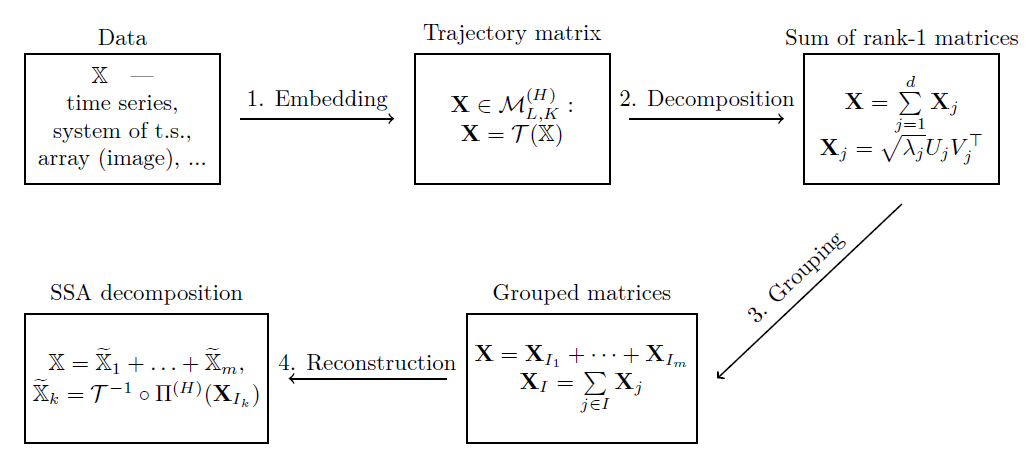
\includegraphics[width = 6in]{scheme_ssa}
	\end{center}
	\caption{Схема SSA-подобных алгоритмов.}
	\label{fig:ssa_scheme}
\end{figure}
\paragraph{Шаг 1. Вложение.} Первый шаг заключается в построении так называемой \textit{траекторной матрицы} $\mathbf{X} = \mathcal{T}\left(\mathbb{X} \right)$ с помощью оператора $\mathcal{T}$.
Обозначим $\mathcal{M}_{L,K}$ --- множество (вещественных или комплексных в случае CSSA) матриц размера $L \times K$, и за $\mathcal{M}_{L,K}^{(H)}$ --- множество (вещественных или комплексных в случае CSSA) ганкелевых матриц размера $L \times K$.
На данном шаге для каждого метода надо определить оператор $\mathcal{T}$ или траекторную матрицу $\mathbf{X}$.
Далее приведен  вид  оператора $\mathcal{T}$ или траекторной матрицы $\mathbf{X}$ для всех вариантов SSA-подобных методов.
\begin{enumerate}
\item 1D-SSA и одномерный вещественный ряд $\mathbb{X}= (x(1),\ldots,x(N))$ длины $N$.

Оператор $\mathcal{T}$ действует из пространства $\mathsf{R}^N$ в пространство $\mathcal{M}_{L,K}^{(H)}$ ганкелевых матриц размера $L \times K$:
\begin{equation*}
\mathcal{T}_{\text{1D-SSA}}(\mathbb{X}) = \begin{pmatrix}
			x(1) & x(2) & x(3) & \ldots & x({K}) \\
			x(2) & x(3) & x(4) & \ldots & x({K+1}) \\
			x(3) & x(4) & x(5) & \ldots & x({K+2}) \\
			\vdots &\vdots & \vdots & \ddots & \vdots \\
			x({L}) & x({L+1}) & x({L+2}) & \ldots & x({N})
			\end{pmatrix},
\end{equation*}

где $1<L<N$ называется \textit{длиной окна}, $K=N-L+1$.
\item CSSA и комплексный ряд $\mathbb{X}=\mathbb{X}^{(1)} + \I \,\mathbb{X}^{(2)}= \left(x^{(1)}(1) + \I\,x^{(2)}(1) ,\ldots,x^{(1)}(N) + \I\,x^{(2)}(N)\right)$.

Оператор $\mathcal{T}$ действует из пространства $\mathsf{C}^N$ в пространство $\mathcal{M}_{L,K}^{(H)}$ комплексных ганкелевых матриц размера $L \times K$, и траекторная матрица имеет такой же вид, как для 1D-SSA, только является комплексной.

\item MSSA и система $\mathbb{X}=\left(\mathbb{X}^{(1)},
 \ldots,\mathbb{X}^{(s)}\right)$ из $s$ временных рядов длины $N_p$, $\mathbb{X}^{(p)} = \left( x^{(p)}(j) \right)_{j=1}^{N_p}$, $p=1,\ldots,s$.

 В данном случае длиной окна $L$ будем называть $1< L < \min(N_p,p=1,\ldots,s)$. Определим также $K_p = N_p - L + 1$, $K = \sum_{p=1}^{s} K_p$. Траекторная матрица для многомерного ряда $\mathbb{X}$ --- это матрица размера $L \times K$ и вида
\begin{gather*}
\mathcal{T}_{\text{MSSA}} = \mathbf{X} = \left[ \mathbf{X}^{(1)}: \ldots :  \mathbf{X}^{(s)}  \right],
\end{gather*}
где $\mathbf{X}^{(p)}= \mathcal{T}_{\text{1D-SSA}} \left(\mathbb{X}^{(p)} \right)$ --- траекторная матрица одномерного ряда $\mathbb{X}^{(p)}$.
Другими словами, траекторная матрица многомерного ряда $\mathbb{X}$ представляет собой расположенные последовательно траекторные матрицы $\mathbf{X}^{(1)},\ldots, \mathbf{X}^{(s)}$ рядов $\mathbb{X}^{(1)}, \ldots, \mathbb{X}^{(s)}$.

\item 2D-SSA и поле $\mathbb{X}= \left(x(i,j) \right)_{i,j=1}^{N_x,N_y}$.

В этом случае длиной окна будем называть $(L_x, L_y)$, удовлетворяющие условиям $1 \leqslant L_x \leqslant N_x$, $1 \leqslant L_y \leqslant N_y$, $1 \leqslant L_x L_y \leqslant N_x N_y$. Положим $K_x = N_x - L_x + 1$ и $K_y = N_y - L_y + 1$. Также определим $L = L_x L_y$, $K = K_x K_y$.

Траекторная матрица для поля $\mathbb{X}$ --- это матрица размера $L \times K$ и вида
\begin{equation*}
\mathcal{T}_{\text{2D-SSA}}(\mathbb{X}) = \mathbf{X}= \begin{pmatrix}
			\mathbf{H}_1 & \mathbf{H}_2 & \mathbf{H}_3 & \ldots & \mathbf{H}_{K_y} \\
			\mathbf{H}_2 & \mathbf{H}_3 & \mathbf{H}_4 & \ldots & \mathbf{H}_{K_y+1} \\
			\mathbf{H}_3 & \mathbf{H}_4 & \mathbf{H}_5 & \ldots & \mathbf{H}_{K_y+2} \\
			\vdots &\vdots & \vdots & \ddots & \vdots \\
			\mathbf{H}_{L_y} & \mathbf{H}_{L_y+1} & \mathbf{H}_{L_y+2} & \ldots & \mathbf{H}_{N_y}
			\end{pmatrix}.
\end{equation*}
Матрица является блочно-ганкелевой с ганкелевыми блоками размера $L_x \times K_x$
\begin{equation*}
\mathbf{H}_j = \mathcal{T}_{\text{1D-SSA}}(\mathbb{X}_{:j})  = \begin{pmatrix}
			x(1,j) & x(2,j) & \ldots & x(K_x, j) \\
			x(2,j) & x(3,j) & \ldots & x(K_x+1, j) \\
			\vdots  & \vdots & \ddots & \vdots \\
			x(L_x, j) & x(L_x+1, j) & \ldots & x(N_x, j)
			\end{pmatrix},
\end{equation*}
где $\mathbb{X}_{:j}$ --- $j$-ый столбец матрицы $\mathbb{X}$.
\end{enumerate}

\paragraph{Шаг 2. Сингулярное разложение.}
На данном этапе происходит сингулярное разложение (SVD) матрицы $\mathbf{X}$ в сумму $d$ элементарных матриц
\begin{equation} \label{eq:svd}
    \mathbf{X}=\mathbf{X}_1+\ldots+\mathbf{X}_d,
\end{equation}
где
$\mathbf{X}_i=\sqrt{\lambda_i}U_i V_i^\mathrm{*}$, $d=\max\{i : \lambda_i > 0\}$,
$\lambda_1,\ldots,\lambda_d$ --- положительные собственные числа, взятые в неубывающем порядке $(\lambda_1\geqslant\ldots\geqslant\lambda_d\geqslant 0)$, и $U_1,\ldots,U_d$ --- соответствующие им ортонормированные собственные вектора матрицы  $\mathbf{X}\mathbf{X}^\mathrm{*}$, $V_i=\mathbf{X}^\mathrm{*} U_i/\sqrt{\lambda_i}$, $\mathrm{*}$ обозначает эрмитово сопряжение, что является операцией транспонирования для всех SSA методов кроме CSSA. 
Обычно в реальных примерах $d=L$.

Числа $\sqrt{\lambda_i}$ называются \emph{сингулярными числами}, $U_i$  и $V_i$ --- \emph{левыми} и \emph{правыми сингулярными векторами} матрицы  $\mathbf{X}$ соответственно.

\paragraph{Шаг 3. Группировка.}  Процедура группировки делит все множество индексов ${1,\ldots,d}$, полученных в результате разложения \eqref{eq:svd}, на $m$ не пересекающихся подмножеств $I_1,\ldots,\\ I_m$.
Результирующая матрица $\mathbf{X}_I$, соответствующая группе $I=\{i_1,\ldots,i_p\}$, определяется как $\mathbf{X}_I=\mathbf{X}_{i_1}+\ldots+\mathbf{X}_{i_p}$.
Вычислив такие матрицы для всех групп $I=I_1,\ldots,I_m$, получаем сгруппированный вид представления \eqref{eq:svd}:
\begin{equation}\label{eq:svd_group}
    \mathbf{X}=\mathbf{X}_{I_1}+\ldots+\mathbf{X}_{I_m}.
\end{equation}

\paragraph{Шаг 4. Восстановление.}
На последнем этапе каждая матрица разложения \eqref{eq:svd_group} переводится в форму исходного объекта $\mathbb{X}$. Преобразование выполняется оптимально в следующем смысле: для матрицы $\mathbf{Y} \in \mathcal{M}_{L,K}$ мы ищем объект $\widetilde{\mathbb{Y}}$, на котором достигается минимум $\|\mathbf{Y} -  \mathcal{T}(\widetilde{\mathbb{Y}})\|_{\mathcal{F}}$, где $\|\mathbf{Z}\|_{\mathcal{F}} = \sqrt{\sum_{i,j=1}^{L,K}(\mathbf{Z})_{ij}^2}$ --- норма Фробениуса.

Обозначим $\Pi^{(H)}: \mathcal{M}_{L,K} \rightarrow \mathcal{M}_{L,K}^{(H)}$ --- ортогональный проектор на $\mathcal{M}_{L,K}^{(H)}$ по норме Фробениуса. Тогда $\widetilde{\mathbb{Y}} = \mathcal{T}^{-1}\left( \Pi^{(H)} \mathbf{Y}\right)$.

Применяем преобразование к результирующим матрицам $\mathbf{X}_{I_k}$ и получаем восстановленные объекты $\widetilde{\mathbb{X}}_k =\mathcal{T}^{-1}\left( \Pi^{(H)} \mathbf{X}_{I_k}\right)$. Таким образом, исходный объект $\mathbb{X}$ раскладывается в сумму $m$ объектов исходного типа
\begin{equation*}
\mathbb{X} = \widetilde{\mathbb{X}}_1 + \ldots + \widetilde{\mathbb{X}}_m.
\end{equation*}
Если $m = d$ и $\mathbf{X}_{I_k} = \mathbf{X}_k$, то восстановленные объекты $\widetilde{\mathbb{X}}_k$ называются \textit{элементарными компонентами}.

\section{Свойства метода 1D-SSA}
\label{sec:1d_ssa_theory}
В данном разделе приведем ряд утверждений про 1D-SSA, которые будем использовать в дальнейшем.

Как уже упоминали во введении, колебательная составляющая описывается суммой э-м гармоник.
Элементы вещественнозначного экспоненциально-модулированного гармонического ряда $\mathbb{S}$ имеют вид
\begin{equation} \label{eq:ex_mod_garm_1d}
 s(n) = a\, e^{\alpha n} \cos(2\pi\omega n + \phi),
\end{equation}
где $0 \leqslant \phi < 2\pi$, $a \not = 0$, $0<\omega \leqslant 0.5$, $\sin \phi \not = 0$ для $\omega = 0.5$.

Введем следующие обозначения: $L$ --- длина окна, параметр метода 1D-SSA, $K=N-L+1$, $\Lambda^{(1)}$ и $\Lambda^{(2)}$ --- подпространства строк и столбцов траекторной матрицы ряда $S_N$.

$L$-Ранг ряда $d$ --- это ранг его траекторной матрицы и, следовательно, количество левых или правых сингулярных векторов, соответствующих ненулевым сингулярным числам траекторной матрицы $\mathbf{X}$.

%Из вида ряда $\mathbb{S}$ и определения траекторной матрицы получается следующее простое утверждение.

\begin{Th} \cite[Утверждение 1]{Zhornikova2016} \label{th:ex_mod_1d}
\begin{enumerate}
\item $L$-Ранг $d$ ряда $\mathbb{S}$, элементы которого имеют вид \eqref{eq:ex_mod_garm_1d},  равен $1$, если $\omega = 0.5$, в остальных случаях $d=2$.
\item Если $\omega \not = 0.5$, то подпространства $\Lambda^{(1)}$ и $\Lambda^{(2)}$ имеют базисы \\
\begin{gather*}
\{(1, e\cos(2\pi\omega),\ldots,e^{\alpha (L-1)}\cos(2\pi (L-1) \omega))^\mathrm{T}, \\
(0, e\sin(2\pi\omega),\ldots,e^{\alpha (L-1)}\sin(2\pi (L-1) \omega))^\mathrm{T}\} \quad \text{и} \\
\{(1, e\cos(2\pi\omega),\ldots,e^{\alpha (K-1)}\cos(2\pi (K-1) \omega))^\mathrm{T}, \\
(0, e\sin(2\pi\omega),\ldots,e^{\alpha (K-1)}\sin(2\pi (K-1) \omega))^\mathrm{T}\}.
\end{gather*}
соответственно.
\item В случае $\omega = 0.5$ одномерные $\Lambda^{(1)}$ и $\Lambda^{(2)}$ натянуты на вектора \\ $(1,c,\ldots,c^{L-1})^{\mathrm{T}}$ и $(1,c,\ldots,c^{K-1})^{\mathrm{T}}$ соответственно, где $c = -e^{\alpha}$.
\end{enumerate}
\end{Th}

\begin{Th} \cite[Предложение 2.3]{Golyandina.etal2003} \label{th:1dssa_num}
Пусть $\alpha = 0$, $\omega \not = 0.5$ и $L\omega$  и $K\omega$ --- целые. Тогда собственные числа сингулярного разложения для ряда $\mathbb{S}$ с элементами вида \eqref{eq:ex_mod_garm_1d} одинаковы и имеют вид $\lambda_1=\lambda_2=a^2LK/4$.
\end{Th}

Из утверждения \ref{th:ex_mod_1d} следует, что для $\omega \not = 0.5$ ряд $\mathbb{S}$ имеет ровно два левых сингулярных вектора $U_1$ и $U_2$, соответствующих ненулевым собственным числам траекторной матрицы,
и что элементы векторов $U_1$ и $U_2$ можно представить в следующем виде:
\begin{gather} \label{eq:vectors_ex_mod_1d}
	u_k^{(1)} = a_1 e^{\alpha k} \cos(2\pi\omega k + \phi_1), \quad u_k^{(2)} = a_2 e^{\alpha k}\cos(2\pi\omega k + \phi_2),
\end{gather}
где $1 \leqslant k \leqslant L$, $0 \leqslant \phi_1, \phi_2 < 2\pi$, $a_1, a_2 \not = 0$.

\begin{Th}  \cite[Утверждение 8]{Zhornikova2016} \label{th:aboutU1U2_ex_mod_1d}
Пусть $\alpha = \alpha_N = C_1/N$, где $C_1$ --- некоторая константа, и $L=[\beta N]$, где $0<\beta<1$. Тогда для сингулярных векторов $U_1$ и $U_2$ ряда $\mathbb{S}$, элементы которых имеют вид \eqref{eq:vectors_ex_mod_1d}, выполняются соотношения: $\lim_{L \rightarrow \infty}{|\phi_1-\phi_2|}=\pi/2 \,\,(\mod \pi)$ и $\lim_{L \rightarrow \infty}{(a_1/a_2)} = 1$.
\end{Th}


Введем определение периодограммы ряда $\mathbb{Y}=(y(1),\ldots,y({M}))$ длины M:
\begin{gather}
\label{eq:per}
 \Pi_{\mathbb{Y}}^M(k/M) = \frac{M}{2}
\begin{cases}
2c_0^2 &\quad \text{для } k = 0, \\
c_k^2 + s_k^2 & \quad \text{для }  0 \leqslant k \leqslant M/2, \\
2c_{M/2}^2 & \quad \text{для } k = M/2   \text{, если } M \text{ четное},
\end{cases}
\end{gather}
где коэффициенты $c_k$ и $s_k$ получаются из разложения Фурье для ряда $\mathbb{Y}$:
\begin{gather*}
y(n) = c_0 + \sum_{k=1}^{\lfloor M/2 \rfloor}\left(c_k\cos(2\pi n k /M) + s_k\sin(2\pi n k/M) \right).
\end{gather*}

\begin{Th}  \cite[Утверждение 3.1]{Alexandrov2006} \label{th:aleks1}
Пусть $\alpha = 0$, $\omega \not = 0.5$ и $L\omega \in \mathsf{Z}$. Тогда для сингулярных векторов $U_1$, $U_2$ ряда $\mathbb{S}$, элементы которого имеют вид \eqref{eq:ex_mod_garm_1d}, выполняется
\begin{gather*}
\max_{0 \leqslant k \leqslant L} \Pi_{U_1}(k/L) = \max_{0 \leqslant k \leqslant L} \Pi_{U_2}(k/L) =  \Pi_{U_1}(\omega) =  \Pi_{U_2}(\omega) = 1,
\end{gather*}
причем для любого другого сингулярного вектора $W_j$ $(j = 1,\ldots, L)$ любого другого ряда $\mathbb{R} \not = \mathbb{S}$ будет выполняться
\begin{gather*}
\max_{0 \leqslant k \leqslant L} \Pi_{W_j}(k/L) < 1.
\end{gather*}
\end{Th}

Пусть $P = (p_1,\ldots,p_L)^{\mathrm{T}}$ и $Q=(q_1,\ldots,q_L)^{\mathrm{T}}$ --- два вещественных вектора длины $L$. Введем для них меру 
\begin{gather} \label{eq:tau1} 
\tau(P, Q) := \hat{\D}(\Theta) =\frac{1}{L-1}\sum_{k=1}^{L-1}{\left(\theta_k  - \bar{\theta}\right)^2},
\end{gather}
где $\Theta=(\theta_1,\ldots,\theta_L)^{\mathrm{T}}$,
$\bar{\theta} = \sum_{k=1}^{L-1}{\theta_k}/(L-1)$, $\theta_k$ --- угол между  
$\left(p_k, q_{k}\right)^{\mathrm{T}}$ и $\left(p_{k+1}, q_{k+1}\right)^{\mathrm{T}}$, т.е.
\begin{gather*}
\theta_k = \arccos{\left(\frac{p_{k} p_{k+1} + q_{k} q_{k+1}}{\sqrt{p_{k}^2+q_{k}^2}\sqrt{p_{k+1}^2+q_{k+1}^2}}\right)}.
\end{gather*}

\begin{Th}  \cite[Теорема 1]{Zhornikova2016} \label{th:th_tau_1d}
Для сингулярных векторов $U_1$ и $U_2$  ряда $\mathbb{S}$, элементы которых имеют вид \eqref{eq:vectors_ex_mod_1d}, верны следующие утверждения.
\begin{enumerate}
\item \label{th:re_tau1}
Если $\alpha=0$ и $L\omega$ --- целое, то $\tau(U_1, U_2)=0$.
\item \label{th:re_tau2}
Если $\alpha = 0$ и  $L=[\beta N]$, где $0<\beta<1$, то $\lim_{L \rightarrow \infty}\tau(U_1, U_2) = 0$.
\item  \label{th:re_tau3}
Если $\alpha = \alpha_N = C_1/N$, где $C_1$ --- некоторая константа, и $L=[\beta N]$, где $0<\beta<1$, то $\lim_{L \rightarrow \infty}\tau(U_1, U_2) = 0$.
\end{enumerate}
\end{Th}

\section{Свойства метода CSSA}
\label{sec:cssa_theory}
Аналогично, как в предыдущем разделе, приведем здесь теоретические утверждения, относящиеся к CSSA.

%В комплексном случае, аналогично, как и в вещественном, определим \textit{колебательную составляющую} как сумму комплексных э-м гармоник.
Рассмотрим \textit{комплекснозначный экспоненциально-модулированный гармонический ряд} $\mathbb{S}$, т.е. ряд с элементами:
\begin{equation} \label{eq:complex_exmodgarm}
 s(n) = e^{\alpha n} (a\cos(2\pi\omega n + \phi_1) + \I \,b\cos(2\pi\omega n + \phi_2)),
\end{equation}
где $0 \leqslant\phi_1, \phi_2 < 2\pi$, $a, b \not = 0$, $0<\omega \leqslant 0.5$, $\sin \phi_1 \not = 0$ или $\sin \phi_2 \not = 0$ для $\omega = 0.5$.

По-прежнему, $L$ --- длина окна, $K=N-L+1$, $\Lambda^{(1)}$ и $\Lambda^{(2)}$ --- подпространства строк и столбцов траекторной матрицы ряда $\mathbb{S}$, $d$ --- $L$-ранг ряда $\mathbb{S}$.

%Так же, как и в вещественном случае, из вида ряда $\mathbb{S}$ и определения траекторной матрицы получается следующее простое утверждение.

\begin{Th} \cite[Утверждение 3]{Zhornikova2016} \label{th:cssa_ex_mod_im_vec}
\begin{enumerate}
\item $L$-ранг $d$ ряда $\mathbb{S}$, элементы которого имеют вид \eqref{eq:complex_exmodgarm},  равен $1$, если $a=b$ и $|\phi_1 - \phi_2| = \pi/2 \,\,(\mod \pi)$ или $\omega = 0.5$, в остальных случаях $d=2$.
\item Если $\omega$ и $\phi_j$ такие, что $d = 2$, то пространства $\Lambda^{(1)}$ и $\Lambda^{(2)}$ имеют базисы
\begin{gather*}
\{(1, e\cos(2\pi\omega),\ldots,e^{\alpha (L-1)}\cos(2\pi (L-1) \omega))^{\mathrm{T}}, \\
(0, e\sin(2\pi\omega),\ldots,e^{\alpha (L-1)}\sin(2\pi (L-1) \omega))^{\mathrm{T}}\},  \quad \text{и} \\
\{(1, e\cos(2\pi\omega),\ldots,e^{\alpha (K-1)}\cos(2\pi (K-1) \omega))^{\mathrm{T}}, \\
(0, e\sin(2\pi\omega),\ldots,e^{\alpha (K-1)}\sin(2\pi (K-1) \omega))^{\mathrm{T}}\}
\end{gather*}
соответственно.
\item Если
%$\omega$ и $\phi_i$ такие, что $d=1$,
 $a=b$ и $|\phi_1 - \phi_2| = \pi/2 \,\,(\mod \pi)$ одномерные пространства $\Lambda^{(1)}$ и $\Lambda^{(2)}$ натянуты на вектора $(1,c,\ldots,c^{L-1})^{\mathrm{T}}$ и $(1,c,\ldots,c^{K-1})^{\mathrm{T}}$ соответственно, где $c = e^{\I 2\pi\omega + \alpha}$. Если $\omega = 0.5$ одномерные $\Lambda^{(1)}$ и $\Lambda^{(2)}$ натянуты на вектора $(1,c,\ldots,c^{L-1})^{\mathrm{T}}$ и $(1,c,\ldots,c^{K-1})^{\mathrm{T}}$ соответственно, где $c = -e^{\alpha}$.
\end{enumerate}
\end{Th}

 Из утверждения \ref{th:cssa_ex_mod_im_vec} следует, что если $\omega$ и $\phi_j$ такие, что $d = 2$, то элементы сингулярных векторов $U_1$ и $U_2$ ряда $\mathbb{S}$ можно представить в следующем виде:
\begin{gather} \label{eq:uuu1}
	u_k^{(1)} = a_1 e^{\alpha k} \cos(2\pi\omega k + \phi_1) + \I \, b_1 e^{\alpha k} \cos(2\pi\omega k + \psi_1),\\ \label{eq:uuu2}
	u_k^{(2)} = a_2 e^{\alpha k}\cos(2\pi\omega k + \phi_2)+ \I \, b_2 e^{\alpha k} \cos(2\pi\omega k + \psi_2),
\end{gather}
где $1 \leqslant k \leqslant L$, $0 \leqslant \phi_j, \psi_j < 2\pi$, $a_j, b_j \not = 0$, $j=1,2$.

\begin{Th} \cite[Предложение 2.3]{Golyandina.etal2003} \label{th:cssa_num}
Пусть $\alpha = 0$, $\omega \not = 0.5$, $L\omega$ и $K\omega$ --- целые. Тогда
\begin{enumerate}
\item для комплексной гармоники $\mathbb{S}$, элементы которой имеют вид \eqref{eq:complex_exmodgarm}, в случае $d=2$ собственные числа имеют вид  $D^2LK$ и $E^2LK$, где
\begin{equation*}
D^2=(a^2+b^2-2ab\sin\phi)/4, \quad E^2=(a^2+b^2+2ab\sin\phi)/4
\end{equation*}
и $\phi=\phi_2-\phi_1$;
\item для комплексной гармоники $\mathbb{S}$, элементы которой имеют вид \eqref{eq:complex_exmodgarm}, в случае $d=1$ собственное число имеет вид $\lambda=a^2LK$.
\end{enumerate}
\end{Th}

Определение \eqref{eq:tau1} для меры $\tau$, используемое ниже в утверждении, дано в предыдущем разделе \ref{sec:1d_ssa_theory}.
\begin{Th}   \cite[Теорема 2]{Zhornikova2016} \label{th:th_tau_cssa}
Пусть $U_1$ и $U_2$ --- сингулярные вектора для ряда $\mathbb{S}$ с рангом $d=2$, записанные в виде \eqref{eq:uuu1} и \eqref{eq:uuu2} соответственно. Тогда верны следующие утверждения.
\begin{enumerate}
\item \label{th:complex_t_1}
Если $\alpha=0$ и $L\omega$ --- целое, то существует $0 \leqslant t < 1$, такое что
\begin{gather*}
\tau(\RE U_1, \RE e^{\I 2\pi t} U_2) + \tau_1 (\IM U_1, \IM e^{\I 2\pi t} U_2) = 0.
\end{gather*}
\item \label{th:complex_t_4}
Если $\alpha = 0$ и $L=[\beta N]$, где $0<\beta<1$, то существует числовая последовательность $t = t_L$, принимающая значения в $[0,1)$, такая что
\begin{gather*}
\lim_{L \rightarrow \infty} (\tau (\RE U_1, \RE e^{\I 2\pi t} U_2) + \tau (\IM U_1, \IM e^{\I 2\pi t} U_2)) = 0.
\end{gather*}
\item \label{th:complex_t_5}
Если $\alpha = \alpha_N = C_1/N$, где $C_1$ --- некоторая константа, и $L=[\beta N]$, где $0<\beta<1$, то существует числовая последовательность $t = t_L$, принимающая значения в $[0,1)$, такая что
\begin{gather*}
\lim_{L \rightarrow \infty} (\tau (\RE U_1, \RE e^{\I 2\pi t} U_2) + \tau (\IM U_1, \IM e^{\I 2\pi t} U_2)) = 0.
\end{gather*}
\end{enumerate}
\end{Th}

Для случая $d=1$, т.е. когда в \eqref{eq:complex_exmodgarm} $a=b$ и $|\phi_1 - \phi_2| = \pi/2 \,\,(\mod \pi)$ обозначим единственный сингулярный вектор, соответствующий ненулевому сингулярному числу, как $U_1$.
По утверждению \ref{th:cssa_ex_mod_im_vec} элементы сингулярного вектора $U_1$ имеют вид
\begin{gather} \label{eq:vid_d1}
	u_k^{(1)} = c\,e^{2\pi \mathrm{i} \omega k + \alpha k},
\end{gather}
где $c$ --- некоторая константа.

\begin{Th}  \cite[Утверждение 14]{Zhornikova2016} \label{th:th_tau_cssa_d1}
Для сингулярного вектора $U_1$ ряда $S_N$ с рангом $d=1$, записанного в виде \eqref{eq:vid_d1},
 \begin{gather*}
 \tau_1(\RE U_1, \IM U_1)=0.
 \end{gather*}
\end{Th}

%\begin{remark}
%Утверждения \ref{th:cssa_ex_mod_im_vec} и \ref{th:cssa_num} демонстрируют важные различия между вещественным и комплексным вариантами SSA для гармонических рядов. Во-первых, в случае  CSSA для ситуации с $0 < \omega < 0.5$, если ряды имеют одинаковые амплитуды, а их фазы отличаются на $\pi/2$, то мы приходим к сингулярному разложению с одним слагаемым, в то время как 1D-SSA всегда даёт сингулярное разложение с двумя слагаемыми. Во-вторых, для CSSA собственные числа, как правило, различны (при целых $L\omega$  и  $K\omega$ они одинаковы только если ряды софазные или противофазные), в то время как при тех же условиях на $L$, $K$ и $\omega$ 1D-SSA дает одинаковые собственные числа.
%\end{remark}

\section{Свойства метода MSSA}
\label{sec:mssa_theory}
В данном разделе приведем теоретические утверждения, относящиеся к MSSA.

Рассмотрим \textit{многомерный экспоненциально-модулированный гармонический ряд} $\mathbb{S} = \left(\mathbb{S}^{(1)},
 \ldots,\mathbb{S}^{(s)}\right)$, где элемент $p$-го ряда имеет вид
\begin{equation} \label{eq:em_mssa}
 s^{(p)}(n) = e^{\alpha n} a_p\cos(2\pi\omega n + \phi_p),
\end{equation}
где $0 \leqslant\phi_p < 2\pi$, $a_p \not = 0$, $0<\omega \leqslant 0.5$, $\sin \phi_p \not = 0$ для $\omega = 0.5$, $n=1,\ldots,N_p$, $p=1,\ldots,s$.

$L$ --- длина окна, $K_p = N_p - L + 1$, $K = \sum_{p=1}^{s} K_p$.
% $\Lambda^{(1)}$ и $\Lambda^{(2)}$ --- подпространства столбцов и строк траекторной матрицы ряда $\mathbb{S}$ соответственно, $d$ --- $L$-ранг ряда $\mathbb{S}$.

%Из вида ряда $\mathbb{S}$ и определения траекторной матрицы получается следующее  утверждение.

\begin{Th}  \cite[Предложение 2.2]{Golyandina.etal2003} \label{th:mssa_num} \label{th:mssa_vec}
\begin{enumerate}
\item 
$L$-Ранг $d$ ряда $\mathbb{S}$, элементы которого задаются \eqref{eq:em_mssa}, равен $1$, если $\omega = 0.5$, в остальных случаях $d=2$.
\item Если $\omega \not = 0.5$, то подпространство $\Lambda^{(1)}$ имеет базис 
\begin{gather*}
\{(1, e\cos(2\pi\omega),\ldots,e^{\alpha (L-1)}\cos(2\pi (L-1) \omega))^\mathrm{T}, \\
(0, e\sin(2\pi\omega),\ldots,e^{\alpha (L-1)}\sin(2\pi (L-1) \omega))^\mathrm{T}\}. 
\end{gather*}
\item Если $\omega \not = 0.5$, то подпространство $\Lambda^{(2)}$ имеет базис 
\begin{gather*}
\{(c^{(1)}_1,\ldots,c_{K_1}^{(1)}; \ldots; c^{(s)}_1,\ldots,c_{K_s}^{(s)})^\mathrm{T},
(d^{(1)}_1,\ldots,d_{K_1}^{(1)}; \ldots; d^{(s)}_1,\ldots,d_{K_s}^{(s)})^\mathrm{T} \}, 
\end{gather*}
где 
\begin{gather*}
c^{(p)}_j = a_p \cos(2\pi j \omega + \phi_p) \quad \text{и}\quad d^{(p)}_j = a_p \sin(2\pi j \omega + \phi_p), \quad j=1,\ldots,K_p, \quad, p=1,\ldots,s.
\end{gather*}
\item В случае $d=1$ одномерные $\Lambda^{(1)}$ и $\Lambda^{(2)}$ натянуты на вектора \\ $(1,c,\ldots,c^{L-1})^{\mathrm{T}}$ и $(1,c,\ldots,c^{K-1})^{\mathrm{T}}$ соответственно, где $c = -e^{\alpha}$.
\end{enumerate}
\end{Th}

\begin{Th} \cite[Предложение 2.3]{Golyandina.etal2003} \label{th:mssa_num}
Пусть $\alpha = 0$, $\omega \not = 0.5$ и $L\omega$  и $K\omega$ --- целые, $s=2$. Тогда собственные числа сингулярного разложения для двумерного ряда ряда $\mathbb{S}$, элементы которого задаются \eqref{eq:em_mssa}, одинаковы и имеют вид $\lambda_1=\lambda_2=(a^2 + b^2)LK/4$.
\end{Th}

\section{Свойства метода 2D-SSA}
\label{sec:2d_ssa_theory}
В данном разделе приведем теоретические утверждения, относящиеся к 2D-SSA.

Согласно \cite{Golyandina.Usevich2010} определим элементы двумерной гармоники $\mathbb{S}$ с частотами $\omega^{(X)}$, $\omega^{(Y)}$:
\begin{gather} \label{eq:2d_cos_el}
\notag
s(k,l) =  \left(
\begin{matrix}
\cos(2\pi \omega^{(X)}k) \\ \notag
\sin(2\pi \omega^{(X)}k)
\end{matrix}
\right)^{\mathrm{T}}
 \left(
\begin{matrix}
a & b \\
c & d
\end{matrix}
\right)
 \left(
\begin{matrix}
\cos(2\pi \omega^{(Y)}l) \\ \notag
\sin(2\pi \omega^{(Y)}l)
\end{matrix}
\right),
\notag
\end{gather}
где $1 \leqslant k \leqslant N_x$, $1 \leqslant l \leqslant N_y$, хотя бы один коэффициент из  группы $\{a,b,c,d\}$ не равен нулю и
$\omega^{(X)}, \omega^{(Y)} \in (0,0.5)$.

Колебательная составляющая --- это сумма $\mathbb{H}$ какого-то числа $c$ двумерных гармоник. Элементы $\mathbb{H}$ имеют вид
\begin{gather} \label{eq:2d_cos}
h(k,l) = \sum_{m=1}^{c}{s_m(k,l)},
\end{gather}
где $a_m(k,l)$ --- элементы гармоники $\mathbb{S}_m$, $m=1,\ldots,c$.
\begin{gather}
\notag
h(k,l) = \sum_{m=1}^{c}(a \cos(2\pi \omega^{(X)}k) \cos(2\pi \omega^{(Y)}l) +
b_m \cos(2\pi \omega^{(X)}k) \sin(2\pi \omega^{(Y)}l) + \\ \label{eq:2d_cos_el}
c_m \sin(2\pi \omega^{(X)}k) \cos(2\pi \omega^{(Y)}l) +
d_m \sin(2\pi \omega^{(X)}k) \sin(2\pi \omega^{(Y)}l)),
\end{gather}
где $1 \leqslant k \leqslant N_x$, $1 \leqslant l \leqslant N_y$, хотя бы один коэффициент из каждой группы $\{a_m,b_m,c_m,d_m\}$ не равен нулю, а также выполняются условия
\begin{align} \label{eq:2d_omega}
\begin{matrix}
(\omega_n^{(X)}, \omega_n^{(Y)}) \not = (\omega_m^{(X)}, \omega_m^{(Y)}), \quad \text{для } n \not= m,\\
\omega_m^{(X)}, \omega_m^{(Y)} \in (0,0.5).
\end{matrix}
\end{align}

\begin{Th}[\cite{Golyandina.Usevich2010}, Proposition 4.7] \label{th:2d_rank_cos}
Для длины окна $(L_x, L_y)$ такой, что $L_x, L_y, K_x, \\K_y \geqslant 4c$ ряд $\mathbb{H}$, элементы которого определены в \eqref{eq:2d_cos_el}, является рядом конечного ранга и его ранг равен
\begin{gather*}
\rank_{L_x, L_y}(\mathbb{H}) = \sum_{m=1}^{c}{\nu_m}, \quad \text{где } \nu_m=2\rank
 \left(
  \begin{matrix}
a_m &b_m &c_m &d_m \\
d_m &-c_m &-b_m &a_m
\end{matrix}
\right).
\end{gather*}
\end{Th}

\section{Разделимость}
\label{sec:separability}
Очень важным понятием в теории SSA является разделимость. Пусть $\mathbb{X} = \mathbb{X}_1 + \mathbb{X}_2$. \textit{(Приближенная) разделимость} означает, что существует такая группировка, что восстановленный ряд $\widetilde{\mathbb{X}}_1$ (приблизительно) равен ряду $\mathbb{X}_1$.
Свойства сингулярного разложения в качестве условий разделимости дают (приближенную) ортогональность столбцов и строк траекторных матриц $\mathbf{X}_1$  и  $\mathbf{X}_2$ объектов $\mathbb{X}_1$ и $\mathbb{X}_2$ соответственно.

Введем формальное определение разделимости.
Пусть  $\mathbb{X}_1$,  $\mathbb{X}_2$ --- два объекта одного типа. Выберем некоторую длину окна $L$. Обозначим за $\mathbf{X}_1$  и  $\mathbf{X}_2$ траекторные матрицы объектов $\mathbb{X}_1$,  $\mathbb{X}_2$ соответственно.

Обозначим  $\Lambda^{(L,1)}$  и $\Lambda^{(L,2)}$  линейные пространства, порожденные столбцами траекторных матриц   $\mathbf{X}^{(1)}$  и  $\mathbf{X}^{(2)}$  соответственно. Аналогичные обозначения  $\Lambda^{(K,1)}$  и $\Lambda^{(K,2)}$  будем использовать для пространств, порожденных столбцами эрмитово сопряженных матриц $(\mathbf{X}^{(1)})^\mathrm{*}$  и  $(\mathbf{X}^{(2)})^\mathrm{*}$.

\begin{defn}
Объекты $\mathbb{X}_1$,  $\mathbb{X}_2$ называются \emph{слабо разделимыми}, если пространство $\Lambda^{(L,1)}$ ортогонально пространству $\Lambda^{(L,2)}$, и пространство $\Lambda^{(K,1)}$  ортогонально пространству $\Lambda^{(K,2)}$.
\end{defn}

\begin{defn}
Пусть объекты $\mathbb{X}_1$,  $\mathbb{X}_2$ слабо разделимы, и множество собственных чисел разложения
 траекторной матрицы одного ряда не пересекается с множеством собственных чисел сингулярного разложения второго ряда,
 тогда объекты $\mathbb{X}_1$,  $\mathbb{X}_2$ называются \emph{сильно разделимыми}.
\end{defn}

Например, в 1D-SSA э-м гармоника приближенно отделима от любой другой э-м гармоники, от экспоненты и от полиномиального или константного ряда.

\subsection{Характеристика разделимости}
\label{sec:sep}
Чтобы проверить разделимость восстановленных компонент $\widetilde{\mathbb{X}}_1$ и $\widetilde{\mathbb{X}}_2$, мы должны проверить ортогональность траекторных матриц $\widetilde{\mathbf{X}}_{1}$ и $\widetilde{\mathbf{X}}_{2}$, им соответствующих. Удобной мерой их ортогональности является скалярное произведение Фробениуса $\langle \widetilde{\mathbf{X}}_{1}, \widetilde{\mathbf{X}}_{2}\rangle_\mathcal{F}$. Нормализованная мера ортогональности: $\rho(\widetilde{\mathbf{X}}_{1}, \widetilde{\mathbf{X}}_{2}) = \langle \widetilde{\mathbf{X}}_{1}, \widetilde{\mathbf{X}}_{2}\rangle_\mathcal{F}/ \left( \| \widetilde{\mathbf{X}}_{1} \|_{\mathcal{F}} \|\widetilde{\mathbf{X}}_{2}\|_{\mathcal{F}} \right)$.

Пусть $\mathbb{E}_k$ --- объект, $k$-ый элемент которого равен 1, а все остальные элементы равны 0. Тогда траекторная матрица $\mathbf{X}$ объекта $\mathbb{X}$ содержит $w(k) := \mathcal{T}(\mathbb{E}_k)$ раз $k$-ый элемент $x(k)$ объекта $\mathbb{X}$. Введем взвешенное скалярное произведение для двух объектов $\mathbb{Y}$ и $\mathbb{Z}$: $(\mathbb{Y}, \mathbb{Z})_w = \sum_k w(k) y(k) z(k)$. Скалярное произведение порождает норму $\|\mathbb{Y}\|_w=\sqrt{(\mathbb{Y}, \mathbb{Y})_w}$. Определим меру
\begin{gather*}
\rho(\widetilde{\mathbf{X}}_{1}, \widetilde{\mathbf{X}}_{2})_w = \frac{\left( \widetilde{\mathbf{X}}_{1}, \widetilde{\mathbf{X}}_{2}\right)_w }{\left( \| \widetilde{\mathbf{X}}_{1} \|_w \|\widetilde{\mathbf{X}}_{2}\|_w \right)},
\end{gather*}
которую будем называть \textit{w-корреляцией}.

Пусть $ \widetilde{\mathbf{X}}_{j}$ --- элементарная восстановленная компонента по элементарной группе $I_j = \{j\}$, тогда матрица с элементами $\rho_{ij}^{w} = \rho(\widetilde{\mathbf{X}}_{i}, \widetilde{\mathbf{X}}_{j})_w$ называется \textit{матрицей w-корреляций}.

\begin{Th} \cite[Corollary 6.2]{Golyandina.etal2001} \label{th:sep_wcor}
Если два вещественных одномерных ряда $\mathbb{X}_1$ и $\mathbb{X}_2$ слабо разделимы, то $(\mathbb{X}_1, \mathbb{X}_2)_w = 0$.
\end{Th}

\chapter{Обзор существующих методов автоматической идентификации для 1D-SSA}
\label{sec:1d_methods}
В данной главе рассматриваем одномерный вещественнозначный временной ряд длины $N$: $\mathbb{X}= (x(1),\ldots,x(N))$, $x(i) \in \mathsf{R}$.

\section{Кластерный метод группировки} \label{sec:1D_wcor}
Данный метод описан в \cite{Golyandina.Zhigljavsky2012} и позволяет делать группировку элементарных компонент.
Будем называть данный метод \textit{кластерным методом группировки}.

%Значение $w(i)$ из \eqref{eq:w_i} --- это количество раз, которое элемент $x(i)$  одномерного вещественного ряда $\mathbb{X}$ появлялся в траекторной матрице
%$\mathbf{X}$.
%Определим скалярное произведение $\left(\mathbb{X}_1, \mathbb{X}_2 \right)_w$ двух одномерных рядов  $\mathbb{X}_1$ и $\mathbb{X}_2$, которое будем называть \textit{w-корреляцией}.
% \begin{equation} \label{eq:1d_w_scalar_prod}
%\left(\mathbb{X}_1, \mathbb{X}_2 \right)_w = \sum_{i=1}^{N}w(i) x_1(i) x_2(i).
%\end{equation}

Метод основан на свойствах матрицы $w$-корреляций $\{\rho^{(w)}_{ij}\}$ между $i$-ой и $j$-ой элементарными восстановленными компонентами, введенной в разделе \ref{sec:sep}.
Для одномерного вещественного ряда $\mathbb{X}$ коэффициенты $w(i)$ принимают вид
\begin{gather} \label{eq:w_i}
 w(i) =
\begin{cases}
i &\quad \text{для } 0 \leqslant i \leqslant L^*, \\
L^* & \quad \text{для } L^* \leqslant i \leqslant K^*, \\
N - i + 1 & \quad \text{для } K^* \leqslant i \leqslant N,
\end{cases}
\end{gather}
где $L^* = \min(L,K)$ и $K^* = \max(L,K)$.
Если взвешенная корреляция $\{\rho^{(w)}_{ij}\}$ имеет большое значение, значит, соответствующие компоненты имеют похожее поведение и должны быть включены в одну группу.

На вход метода поступает матрица $\{\rho^{(w)}_{ij}\}$. Далее к матрице $1 -\{|\rho^{(w)}_{ij}|\}$ применяется метод кластерного анализа, на выходе получается разбиение компонент на группы. Метод реализуется алгоритмом \ref{alg:wcor}.

 \begin{algorithm}[!hhh]
\caption{Кластерный метод автоматической идентификации}
\label{alg:wcor}
\begin{algorithmic}[1]
\REQUIRE матрица w-корреляций $\{\rho^{(w)}_{ij}\}$ между элементарными восстановленными компонентами, количество групп $m$.
\ENSURE Группы индексов компонент.
\STATE  Применяем метод кластерного анализа к матрице $1 -\{|\rho^{(w)}_{ij}|\}$, как матрице расстояний, метод объединения (linkage) --- произвольный.
\STATE Получаем $m$ групп компонент из результатов кластерного анализа.
\end{algorithmic}
\end{algorithm}

Явным недостатком метода является тот факт, что матрица $w$-корреляций не всегда может явно разделяться на отдельные кластеры, и непонятно на сколько устойчивые результаты дает метод, так как в реальных данных мы имеем дело с приближенной разделимостью, и согласно утверждению \ref{th:sep_wcor} раздела \ref{sec:sep} равенство $\left(\mathbb{X}_1, \mathbb{X}_2 \right)_w = 0$ является лишь достаточным условием слабой разделимости.

\section{Кластерный метод выделения сигнала с использованием DFT}
Метод предложен и описан в \cite{Alvarez2013} и позволяет группировать компоненты с похожими частотными характеристиками. Будем называть данный метод \textit{кластерным выделения сигнала с использованием DFT}.

Для начала авторы предлагают метод выбора длины окна $L$.
$L$ выбирают следующим образом: увеличивают значение $\theta$, идя по множеству $\Theta = \{2,\ldots,N -2\}$ до тех пор пока не выполнится:
\begin{gather}
\label{eq:theta_matrix}
\rank(\mathbf{X}^{\theta+1}) < \rank(\mathbf{X}^{\theta}),
\end{gather}
где $\mathbf{X}^{\theta}$ --- траекторная матрица, полученная с помощью $L = \theta$. Как только \eqref{eq:theta_matrix} выполнится, фиксируют $L = \theta$.
%Таким образом, ранг траекторной матрицы будет на единицу больше ранга исходного ряда.

Смысла в описанном выборе окна нет, так как для зашумленного ряда траекторная матрица является матрицей полного ранга.

Далее опишем сам метод, реализуемый алгоритмом \ref{alg:cluster_dft}.
Авторы статьи предполагают, что сингулярные числа шумовой компоненты всегда меньше сингулярных чисел сигнала.
Если уровень шума не очень большой, т.е. сигнал отделяется от шума, то это действительно так. Поэтому на первом шаге метода происходит отбор сингулярных чисел с помощью порога $\tau_\lambda$.

На втором шаге строим матрицу  $\mathbf{\hat U}$ из левых сингулярных векторов, соответствующих сингулярным числам, отобранным на первом шаге. К столбцам матрицы $\mathbf{\hat U}$ применяем дискретное преобразование Фурье (DFT), получаем матрицу $\mathbf{\hat X}$. Авторы отмечают, что вместо DFT можно использовать и другое преобразование, которое будет переводить сингулярный вектор в какую-то его характеристику.

На последнем шаге к столбцам матрицы данных $\mathbf{\hat X}$ применяем кластерный метод, где в качестве расстояния используется евклидова метрика. Авторы пишут, что можно использовать и другую метрику расстояния для кластерного анализа.

 \begin{algorithm}[!hhh]
\caption{Кластерный метод автоматической идентификации с использованием DFT}
\label{alg:cluster_dft}
\begin{algorithmic}[1]
\REQUIRE Порог $\tau_\lambda$.
\ENSURE Группы индексов компонент.
\STATE  $\{ \lambda_1 \geqslant \lambda_2 \geqslant \ldots \geqslant \lambda_{\rank(\mathbf{X})}\}$ --- квадраты сингулярных чисел, соответствующие траекторной матрице $\mathbf{X}$. Выбираем $m$ такое, что $\lambda_m$ --- первый квадрат сингулярного числа, для которого $\lambda_m / \sum_{k=1}^{\rank(\mathbf{X})}\lambda_k < \tau_\lambda$.
\STATE $\mathbf{\hat U}$ --- матрица, составленная из левых сингулярных векторов, соответствующих числам $\{ \lambda_1 \geqslant \lambda_2 \geqslant \ldots \geqslant \lambda_m\}$. К столбцам матрицы $\mathbf{\hat U}$ применяем дискретное преобразование Фурье, получаем матрицу $\mathbf{\hat X}$.
\STATE К столбцам матрицы данных $\mathbf{\hat X}$ применяем кластерный метод, где в качестве расстояния используется евклидова метрика.
\STATE Получаем $m$ групп компонент из результатов кластерного анализа.
\end{algorithmic}
\end{algorithm}

Главный недостаток метода --- непонятно, как выбирать порог  $\tau_\lambda$, так как соотношение сигнала к шуму заранее неизвестно.  В своих примерах авторы использовали $\tau_\lambda = 0.025$.
%В качестве метрики в кластерном методе в статье \cite{Alvarez2013} бралось евклидово расстояние.

\section{Метод низких частот для идентификации тренда}
\label{sec:1d_freq_method}
Данный метод описан в \cite{Golyandina.Zhigljavsky2012}, еще более подробно метод описан в \cite{Alexandrov2006}. Метод позволяет идентифицировать компоненты, относящиеся к тренду.
 Будем называть данный метод \textit{методом низких частот для тренда}.

Метод основан на том, что находит компоненты с похожими частотными характеристиками, как и предыдущий кластерный метод \ref{alg:cluster_dft}. Вклад частоты определяется с помощью периодограммы, определенной для ряда $\mathbb{Y}=(y(1),\ldots,y({M}))$ длины M формулой \eqref{eq:per} в разделе \ref{sec:1d_ssa_theory}:
\begin{gather*}
 \Pi_{\mathbb{Y}}^M(k/M) = \frac{M}{2}
\begin{cases}
2c_0^2 &\quad \text{для } k = 0, \\
c_k^2 + s_k^2 & \quad \text{для }  0 \leqslant k \leqslant M/2, \\
2c_{M/2}^2 & \quad \text{для } k = M/2   \text{, если } M \text{ четное},
\end{cases}
\end{gather*}
где коэффициенты $c_k$ и $s_k$ получаются из разложения Фурье для ряда $\mathbb{Y}$:
\begin{gather*}
y(n) = c_0 + \sum_{k=1}^{\lfloor M/2 \rfloor}\left(c_k\cos(2\pi n k /M) + s_k\sin(2\pi n k/M) \right).
\end{gather*}
Определим для ряда $\mathbb{Y}$ и $0 \leqslant  \omega \leqslant 0.5$ меру
\begin{gather}
\label{eq:T_measure}
T(\mathbb{Y}; \omega) = \sum_{k: 0 \leqslant k/M \leqslant \omega} I_{\mathbb{Y}}^M(k/M),
\end{gather}
где $I_{\mathbb{Y}}^M(k/M) = \Pi_{\mathbb{Y}}^M(k/M) / \|\mathbb{Y}\|^2$, $\Pi_{\mathbb{Y}}^M(k/M)$ определено выше в \eqref{eq:per}. Так как $\|\mathbb{Y}\|^2  = \sum_{k=1}^{\lfloor M/2 \rfloor} \Pi_{\mathbb{Y}}^M(k/M)$, то мера $T(\mathbb{Y}; \omega)$ может рассматриваться как вклад частот, содержащихся в частотном интервале $[0, \omega)$.

Так как тренд --- это низкочастотная составляющая, то для его выделения логично рассматривать частотный интервал $[0, \omega)$, где $\omega$ необходимо выбрать, его нужно брать меньшим значений периодов гармоник, содержащихся в ряде, если они известны.
Для автоматической группировки также нужно выбрать порог $T_0$, и брать те компоненты, значение меры $T$ для которых больше $T_0$.

Получаем алгоритм \ref{alg:freq1d} для частотного метода.

\begin{algorithm}[!hhh]
\caption{1D-SSA. Метод низких частот для тренда}
\label{alg:freq1d}
\begin{algorithmic}[1]
\REQUIRE Значение  $0 \leqslant  \omega \leqslant 0.5$, порог $0 \leqslant T_0 \leqslant 1$, группа индексов $I$, тип рядов $\mathbb{Y}_i$,\\ $i \in I$: левые сингулярные вектора,
правые сингулярные вектора или восстановленные ряды.
\ENSURE Группа индексов компонент $J \subset I$.
\STATE  Для каждого ряда $\mathbb{Y}_i$, $i \in I$, вычисляем значение $T(\mathbb{Y}_i; \omega)$ с помощью \eqref{eq:T_measure}.
\STATE $J$ --- группа индексов $i \in I$, таких что $T(\mathbb{Y}_i; \omega) \geqslant T_0$.
\end{algorithmic}
\end{algorithm}

\section{Парный частотный метод идентификации колебательной компоненты}
\label{sec:1d_pgram_method}

Как мы знаем из введения, колебательная составляющая описывается суммой э-м гармоник.
Рассмотрим алгоритм автоматической идентификации э-м гармоник, предложенный в \cite{Alexandrov2006}.
 Будем называть данный метод \textit{парным частотным методом идентификации колебательной компоненты}.

Метод основан на исследовании периодограмм сингулярных векторов, соответствующих ряду. Метод состоит из двух частей, на первом этапе проводится предварительная проверка, и сингулярные тройки, идентифицированные на этом этапе, проходят дополнительную проверку на втором этапе.
%Будем называть этот метод \textit{периодограммным}.

Как мы знаем из утверждения \ref{th:ex_mod_1d}, в случае 1D-SSA э-м гармоника \eqref{eq:ex_mod_garm_1d} может иметь ранг 1, если частота $\omega=0.5$, или ранг 2 в противном случае, т.е. э-м гармонике может соответствовать либо один сингулярный вектор, либо два.

Описанный далее метод автоматической идентификации компонент, соответствующих э-м гармоникам, проверяет
\begin{itemize}
\item для каждой пары сингулярных векторов тот факт, что последовательности их элементов описываются э-м гармониками с одинаковой частотой,
\item для каждого сингулярного вектора --- что последовательность его элементов описывается э-м гармоникой с периодом 2 ($\omega=0.5$).
\end{itemize}

\begin{remark}
Так как по утверждению \ref{th:1dssa_num} одномерному вещественному гармоническому ряду с $\omega \not = 0.5$ соответствует два равных собственных числа траекторной матрицы, и алгоритм SSA метода, описанный в разделе \ref{sec:ssa_alg}, сортирует компоненты сингулярного разложения по значению собственных чисел, то
для идентификации гармоник ранга 2 достаточно рассматривать только последовательные пары сингулярных векторов.
%По утверждению \ref{th:1dssa_num} одномерному вещественному гармоническому ряду соответствует два равных собственных числа траекторной матрицы, и собственные вектора выдаваемые процедурой из пакета \textsc{Rssa} сортируются по значению собственного числа, поэтому во всех методах идентификации колебательной компоненты рассматриваются  последовательные пары сингулярных векторов.
\end{remark}

Согласно разделу \ref{sec:1d_ssa_theory}, гармоническому ряду вида \eqref{eq:ex_mod_garm_1d} соответствует два сингулярных вектора вида \eqref{eq:vectors_ex_mod_1d} с одинаковыми частотами.

Первый этап метода основан на том факте, что если для гармоники ($\alpha = 0$) с частотой $\omega$ и длины окна $L$ выполняется: $L \omega \in \mathsf{Z}$, то периодограммы ее сингулярных векторов равны $\Pi_{U_j}^L(k/L)=\chi_{\omega}(k/L)$ (где $\chi_{\omega}(\cdot)$ --- индикатор множества $\{\omega\}$).
C учетом наличия только приближенной разделимости, $L\omega \not \in \mathsf{Z}$ и $\alpha \not = 0$,
на первом этапе метода из всех последовательных пар сингулярных векторов выбираются такие, для которых аргументы максимумов периодограмм больше 0 и близки, т.е. отличаются друг от друга не более чем на $s_0/L$ (где $s_0 \in \mathsf{Z}_+$ --- фиксированный параметр метода):
\begin{gather} \label{eq:I_1_P}
I_1^{(\mathbb{P})} = \{ (i, i+1): \quad \theta_1 \theta_2 >0, \quad L |\theta_i - \theta_{i+1}| \leqslant s_0, \quad 1 \leqslant i \leqslant L -1  \},
\end{gather}
где $\theta_j = \argmax_{0 < k \leqslant L/2} \{\Pi_{U_j}^L(k/L)\}$ --- аргумент максимума периодограммы $\Pi_{U_j}^{L}$ сингулярного вектора $U_j$.

Аналогично каждый сингулярный вектор проверяется на соответствие гармонике с периодом 2:
\begin{gather} \label{eq:I_2_P}
I_2^{(\mathbb{P})} = \{i: \quad  L |\theta_{i} - 0.5 | \leqslant s_0, \quad 1 \leqslant i \leqslant L\}.
\end{gather}

Результатом первого этапа являются множества индексов $I_1^{(\mathbb{P})}$ и $I_2^{(\mathbb{P})}$ сингулярных векторов. $I_1^{(\mathbb{P})}$ --- пары номеров сингулярных векторов, идентифицированных как соответствующие э-м гармоникам с $0 < \omega < 0.5$.  $I_2^{(\mathbb{P})}$ --- номера сингулярных векторов, идентифицированных как соответствующие э-м гармонике с $\omega = 0.5$.

\begin{defn} \label{def:rho}
Пусть $\{W_j\}_{j=1}^{L}$, $W_j$ --- вещественные вектора из некоторого множества $A$ векторов, обозначим мощность множества как $\# A$. Введем функцию $\rho_A$, определенную на множестве $A$:
\begin{gather*}
\rho_{A}(k/L) = \frac{1}{\#A} \sum_{W_j \in A}{\Pi^{L}_{W_j}{(k/L)}}.
\end{gather*}
\end{defn}

Ввиду утверждения \ref{th:aleks1} раздела \ref{sec:1d_ssa_theory}, для того чтобы проверить, что сингулярные вектора с номерами $j, j + 1$ соответствуют гармонике, необходимо убедиться, что максимумы их периодограмм достигаются в одной точке, и что каждый из них при этом имеет значение, близкое к 1, так как э-м гармонике с частотой $\omega$: $L \omega \not \in \mathsf{Z}$ тоже соответствует большое значение максимума периодограммы (хоть и меньшее 1), потому что ее периодограмма имеет один четко выраженный пик.  Именно это и проверяется на втором этапе метода.

До работы \cite{Alexandrov2006}, на основе которой мы описываем метод, данный принцип проверки был предложен в работе \cite{Vautard1992}, однако сама идея не нова и была предложена еще в 1929 г. Фишером в статье \cite{Fisher1929}.

Таким образом, на втором этапе метода
 требуется выбрать порог $\rho_0$ для рассматриваемой меры
\begin{gather} \label{eq:rho_ij}
\rho_{i,j} := \max_{0 \leqslant k \leqslant L/2}{\left(\rho_{\{U_i,U_j\}}(k/L) + \rho_{\{U_i,U_j\}}((k+1)/L)\right)},
\end{gather}
где $U_i$, $U_j$ --- пара сингулярных векторов с индексами из множества индексов $I_1^{(\mathbb{P})}$, отобранных на первом этапе.

Для идентификации компонент, относящихся к гармоники ранга 2, мера имеет вид
\begin{gather}\label{eq:rho_i}
\rho_{i} := \rho_{\{U_i\}}((\lfloor L/2 \rfloor)/L) + \rho_{\{U_i\}}((\lfloor L/2 \rfloor + 1)/L),
\end{gather}
где $i \in I_2^{(\mathbb{P})}$.

Итоговым результатом парного частотного метода, реализуемого алгоритмом \ref{alg:1d_pgram}, являются индексы 
\begin{gather} \label{eq:pgram_I_p}
I^{(\mathbb{P})} = \{ (i,j) \in I_1^{(\mathbb{P})}: \rho_{i,j} \geqslant\rho_0 \} \cup \{ i \in I_2^{(\mathbb{P})}: \rho_{i} \geqslant\rho_0 \}.
\end{gather}

\begin{algorithm}[!hhh]
\caption{1D-SSA. Парный частотный метод для колебательной составляющей}
\label{alg:1d_pgram}
\begin{algorithmic}[1]
\REQUIRE Параметр $s_0 \in \mathsf{Z}_{+}$, порог $\rho_0 \in [0,1]$.
\ENSURE Группы индексов компонент.
\STATE  Получаем группу индексов $I_1^{(\mathbb{P})}$ с помощью $s_0$ и \eqref{eq:I_1_P} и группу индексов $I_2^{(\mathbb{P})}$ с помощью $s_0$ и \eqref{eq:I_2_P}.
\STATE Получаем группу индексов $I^{(\mathbb{P})}$ по $\{U_j\}_{j \in I_1^{(\mathbb{P})} \cup I_2^{(\mathbb{P})}}$ и $\rho_0$ с помощью \eqref{eq:pgram_I_p}.
\end{algorithmic}
\end{algorithm}

Автор \cite{Alexandrov2006} советует брать $s_0 = 1$, а для выбора порога $\rho_0$ не дано четких рекомендаций, что является основным недостатком метода. Еще одним недостатком метода является тот факт, что его можно строго обосновать только для немодулированных гармоник ($\alpha = 0$).

\section{Метод группировки Н. В. Абалова, В. В. Губарева}
Метод предложен в статье \cite{Abalov2015} и позволяет делать группировку элементарных компонент. Метод рассматривает пары компонент и относит их к какой-то группе, поэтому в первую очередь метод применим для колебательной компоненты.    Будем называть данный метод \textit{методом группировки Н. В. Абалова, В. В. Губарев}.

Метод комбинирует две идеи. На первом шаге учитывается близость собственных чисел, т.е. вкладов компонент. На втором шаге учитывается похожесть компонент в смысле большой корреляции между ними или близости частот.
Для вещественной гармоники метод легко обосновывается с помощью утверждения \ref{th:1dssa_num} про равные собственные числа и вида сингулярных векторов \eqref{eq:vectors_ex_mod_1d}, имеющих одинаковые частоты.
Опишем общую схему метода.
\begin{enumerate}
\item Для всех элементарных компонент рассчитываем матрицу близости собственных чисел $\Delta = \{\delta_{ij}\}$, $i,j=1,\ldots,d$, где
\begin{gather}
\label{eq:delta}
\delta_{ij} = \frac{\min_{i, j}(\lambda_i, \lambda_j)}{\max_{i,j}(\lambda_i, \lambda_j)}.
\end{gather}
\item Рассчитываем матрицу <<смежности>> компонент $\mathbf{G}=\{g_{ij}\}$, $i,j = 1,\ldots,d$,
\begin{gather} \label{eq:g_ij}
g_{ij}
\begin{cases}
c_{ij}, &\quad \delta_{ij} \geqslant \rho_1, \\
0, &\quad \text{иначе},
\end{cases}
\end{gather}
где $c_{ij}$ --- бинарный показатель близости двух компонент (далее будет рассмотрено два таких показателя  $c^{'}_{ij}$ и  $c^{''}_{ij}$).

Итогом выполнения операций 1--2 является матрица группировки $\mathbf{G}$, содержащая 1 в ячейках $i,j$, если пара компонент $i,j$ принадлежит одной группе, иначе 0.
\item Объединяем в одну группу составляющей ряда те  компоненты, для которых $g_{ij} = 1$.
\end{enumerate}

Первый показатель близости $c_{ij} = c^{'}_{ij}$ основан на использовании
степени коэффициента связи между значениями периодограмм восстановленных компонент $\mathbb{X}_i$, $\mathbb{X}_j$ (например, коэффициента корреляции Пирсона, Спирмена, корреляционных отношений и т.п.). Чем выше значение $\rho_1$, тем жестче отбор.
Здесь $c^{'}_{ij} = 1$ тогда и только тогда, когда $\corr(\mathbb{X}_i, \mathbb{X}_j) \geqslant \rho_c$, $\rho_c \in [0,1]$.

Второй показатель близости $c_{ij} =c^{''}_{ij}$ сравнивает множества частот двух компонент, соответствующих максимальным значениям периодограммы.
Обозначим
$K_{\mathbb{X}_j} = \max_{0\leqslant k \leqslant L/2}\left(\Pi_{\mathbb{X}_j}(k)\right)$ --- максимальное значение периодограммы восстановленной компоненты $\mathbb{X}_j$;
\begin{gather} \label{eq:f_j}
F_{\mathbb{X}_j} =  \{ k: \Pi_{\mathbb{X}_j}(k) \geqslant \rho_p K_{\mathbb{X}_j}  \}, j = 1,\ldots, d.
\end{gather}
Множество $F_{\mathbb{X}_j}$ упорядочено по возрастанию, $\rho_p$ --- задаваемая величина порога, которая позволяет регулировать исключение низких значений периодограмм.

В данном случае $c^{''}_{ij}=1$ тогда и только тогда, когда для любого $h=1,\ldots,m$ имеем $|F_{\mathbb{X}_i}(h) - F_{\mathbb{X}_j}(h)|/ L/2 < \rho_2$, где $F_{\mathbb{X}_i}(h)$ --- $h$-ое значение индекса частоты из множества $F_{\mathbb{X}_i}$, $\rho_2$ --- порог предельного расхождения индекса частот,  $\rho_2 \in [0,1]$, $m = \min\left(\#F_{\mathbb{X}_i}(h), \#F_{\mathbb{X}_j}(h) \right)$. Чем меньше значение $\rho_2$, тем жестче условие.

Авторы статьи говорят, что использование показателя $c^{''}_{ij}$ должно позволить
учесть размытие и слабое смещение пиковых значений периодограмм при повышении уровня шума.
Для примеров авторы статьи брали $\rho_1 =\rho_c =\rho_p = 0.8$, $\rho_2 = 0.05$.

\begin{algorithm}[!hhh]
\caption{1D-SSA. Метод группировки Н. В. Абалова, В. В. Губарева}
\label{alg:1d_abalov}
\begin{algorithmic}[1]
\REQUIRE Параметры $\rho_1, \rho_2, \rho_c, \rho_p  \in [0,1]$.
\ENSURE Группы индексов компонент.
\STATE  С помощью собственных чисел вычисляем матрицу $\Delta = \{\delta_{ij}\}$, $i,j=1,\ldots,d$ по формуле \eqref{eq:delta}.
\STATE Вычисляем матрицу $\mathbf{G}=\{g_{ij}\}$, $i,j = 1,\ldots,d$ по формуле \eqref{eq:g_ij}, где\\
либо $c_{ij} = c_{ij}^{'}$, $c_{ij}^{'} = 1$, если  $\corr(\mathbb{X}_i, \mathbb{X}_j) \geqslant \rho_c$;

либо $c_{ij} = c_{ij}^{''}$, с помощью \eqref{eq:f_j} для каждого $j = 1,\ldots, d$ вычисляем множество $F_{\mathbb{X}_j}$, $c_{ij}^{''} = 1$, если $|F_{\mathbb{X}_i}(h) - F_{\mathbb{X}_j}(h)|/ L/2 < \rho_2$ для любого $h=1,\ldots,m$, $m = \min\left(\#F_{\mathbb{X}_i}(h), \#F_{\mathbb{X}_j}(h) \right)$.
\STATE К одной группе относим те индексы $i,j$, для которых $g_{ij} = 1$.
\end{algorithmic}
\end{algorithm}

Алгоритм \ref{alg:1d_abalov} реализует описанный метод.

Отметим, что если в случае $c_{ij}^{'}$ брать не просто корреляции, а взвешенные корреляции, определение которых дано в разделе \ref{sec:sep}, то получится кластерный метод группировки из раздела \ref{sec:1D_wcor} с некоторыми ограничениями на значения матрицы из-за пункта 1 рассматриваемого алгоритма \ref{alg:1d_abalov}. Если же брать просто корреляции, непонятно почему метод будет работать.


%Основные отличия данного алгоритма от алгоритма из предыдущего раздела.
%\begin{itemize}
%\item
%Вместо строго последовательного попарного рассмотрения
%еще не сгруппированных компонент предлагается рассматривать все
%комбинации пар компонент, имеющих близкие значения собственных
%чисел в соответствии с оценкой \eqref{eq:delta}.
%\item Оценка близости частотного состава осуществляется не по
%совпадению значений частот, соответствующих только одному доминирующему пику в периодограммах собственных векторов, а по одному из двух предложенных критериев, первый из которых позволяет
%учесть весь частотный состав, второй – более одного пика в периодограмме и слабое смещение значений периодограммы из-за
%высокого уровня шума.
%\end{itemize}



\section{Обзор приложений методов}

\subsection{Phil. J. Watson <<Identifying the Best Performing Time Series
Analytics for Sea Level Research>> \cite{Watson2016} \cite{Watson2016b}}

SSA применяется к данным  про уровень морей. Автор выделяет сигнал (средний уровень моря), предполагая, что он нелинейный и нестационарный. Применяется частотный метод автоматической идентификации, реализуемый алгоритмом \ref{alg:freq1d} из раздела \ref{sec:1d_freq_method}, с частотой $\omega=0.01$ и порогом $T_0 = 0.75$.

\subsection{F. Romeroa, F.J. Alonsoa, J. Cuberob, G. Galán-Marína <<An automatic SSA-based de-noising and smoothing technique for surface electromyography signals>>
 \cite{Romeroa2015}}

SSA применяется к данным электромиографии (surface electromyography).
Весь алгоритм анализа довольно длинный, автоматическая идентификация применяется только на одном этапе.
Используется кластерный метод автоматической идентификации, реализуемый алгоритмом \ref{alg:wcor} из раздела \ref{sec:1D_wcor}. К матрице w-корреляций применяется k-means, выбирается группа, для которой средне-квадратичная ошибка с исходным сигналом наименьшая.
%К результату применяется последовательный SSA для избавления от шума и решения проблем разделимости.

\subsection{Michael Leonard and Bruce Elsheimer <<Automatic Singular Spectrum Analysis and Forecasting>>
 \cite{Leonard2017}}

Статья посвящена функциям в языке программирования SAS, позволяющим делать SSA и автоматическую группировку. Снова применяется кластерный метод идентификации  с использованием матриц w-корреляций, реализуемый алгоритмом \ref{alg:wcor}. Группы выбираются таким образом, чтобы в любой группе $I_m$ значение $\rho^{(w)} _{ij}$ было близко к 1 для любых $i, j \in I_m$. Уровень близости к 1 можно задавать с помощью порога: если все корреляции больше этого порога, то значения относятся в одну группу. В пакете по умолчанию выбрано значение для порога $0.9$.

\chapter{Метод идентификации колебательной компоненты по регулярности углов для 1D-SSA}
\label{sec:tau1}
\section{Описание и обоснование метода}
Идея данного метода идентификации колебательной компоненты была предложена в бакалаврской работе \cite{Zhornikova2016} и основывается на свойствах специальной меры, которая была введена в разделе \ref{sec:1d_ssa_theory}.
Приведем определение меры снова.
Для вещественных векторов $P = (p_1,\ldots,p_L)^{\mathrm{T}}$ и $Q=(q_1,\ldots,q_L)^{\mathrm{T}}$ длины $L$: 
\begin{gather*} 
\tau(P, Q) := \hat{\D}(\Theta) =\frac{1}{L-1}\sum_{k=1}^{L-1}{\left(\theta_k  - \bar{\theta}\right)^2},
\end{gather*}
где $\Theta=(\theta_1,\ldots,\theta_L)^{\mathrm{T}}$,
$\bar{\theta} = \sum_{k=1}^{L-1}{\theta_k}/(L-1)$, $\theta_k$ --- угол между  
$\left(p_k, q_{k}\right)^{\mathrm{T}}$ и $\left(p_{k+1}, q_{k+1}\right)^{\mathrm{T}}$, т.е.
\begin{gather*}
\theta_k = \arccos{\left(\frac{p_{k} p_{k+1} + q_{k} q_{k+1}}{\sqrt{p_{k}^2+q_{k}^2}\sqrt{p_{k+1}^2+q_{k+1}^2}}\right)}.
\end{gather*}

По замечанию 3 из  \cite{Zhornikova2016}:
равенство $\tau(P, Q) =0$ означает, что все углы между последовательными точками $(p_k, q_k)^{\mathrm{T}}$ двумерной диаграммы векторов $P$ и $Q$ одинаковые. Если при этом нормы этих векторов монотонно меняются по $k$, то на двумерных диаграммах получатся <<спирали>>.

Таким образом, для $d=2$ в условиях утверждения \ref{th:th_tau_1d} из раздела \ref{sec:1d_ssa_theory} при достаточно больших $L$ по описанному замечанию ряд \eqref{eq:ex_mod_garm_1d} можно идентифицировать с помощью двумерной диаграммы сингулярных векторов $U_1$ и $U_2$ --- она будет обладать свойствами, близкими к свойствам, соответствующих нулевому значению меры $\tau$; если при этом нормы векторов $U_1$ и $U_2$ будут монотонно меняться по $k$, то на двумерных диаграммах получатся <<спирали>>. На рис. \ref{fig:re_ex_mod_diagram} приведены примеры таких изображений для рядов с $N=99$, $L=50$. 

%\begin{figure}[h] 
%    \centering
%   \begin{subfigure}[b]{0.3\textwidth}
%       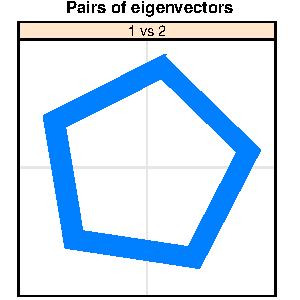
\includegraphics[width=\textwidth]{re_ex_mod_omega_1_5}
%        \caption{
%        \centering $\omega=1/5$, $\alpha = 0.005$, $C_1 = 0.495$, $\tau =$1.3e-05.}
%    \end{subfigure}
%    \begin{subfigure}[b]{0.3\textwidth}
%        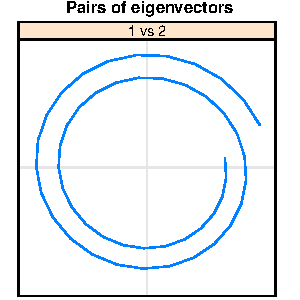
\includegraphics[width=\textwidth]{re_ex_mod_omega_1_25}
%        \caption{ \centering $\omega=1/25$, $\alpha = 0.009$, $C_1 = 0.891$, $\tau =$4.2e-05.}
%    \end{subfigure}
%    \begin{subfigure}[b]{0.3\textwidth}
%        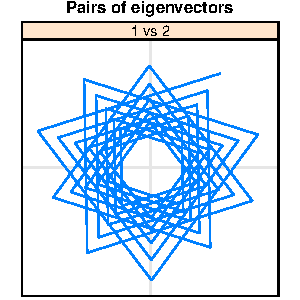
\includegraphics[width=\textwidth]{re_ex_mod_omega_3_10}
%        \caption{ \centering $\omega=3/10$, $\alpha = 0.02$, $C_1 = 1.98$, $\tau =$0.2e-03.}
%    \end{subfigure}
%    \caption{Двумерные диаграммы сингулярных векторов вещественных э.-м. гармоник, $N=99$, $L=50$, $\beta=1/2$.}
%    \label{fig:re_ex_mod_diagram}
%\end{figure} 

%Это свойство соответствуют виду двумерных диаграмм э-м гармоники в случае визуальной идентификации.
%Поэтому рассматриваются значения функционала $\tau$ от пары сингулярных векторов, соответствующих ряду.
Отметим, что на практике мы не имеем дела с рядами бесконечной длины, поэтому для ряда конечной длины $N$ с константным значением $\alpha$ условие $\alpha = C_1/N$ означает не слишком большое значение $e^{\alpha N}$, т.е. ограниченность диапазона изменений значений ряда.


Если число э-м гармоник, которые хотим идентифицировать, известно, то алгоритм состоит просто в отборе пар векторов $U_i$ и $U_{i+1}$ с минимальными значениями функционала  $\tau(U_i, U_{i+1})$, $i=1,\ldots, d-1$.

В случае, когда число
э-м гармоник неизвестно, в работе \cite{Zhornikova2016} было предложено отбирать пары сингулярных векторов с
помощью порога, т.е. к э-м гармонике относить те вектора $U_i$ и $U_{i+1}$, значение  $\tau(U_i, U_{i+1})$ для которых меньше заданного порога, но в работе не было дано никаких обоснований для выбора порога. 
Поэтому в данной главе приведем эмпирические обоснования для выбора порога и проведем численные исследования на примере зашумленного э-м косинуса.    

Отметим, что метод не работает для случая $\omega = 0.5$. Поэтому в данной главе мы его не рассматриваем.

 Будем называть данный метод \textit{методом идентификации колебательной компоненты по регулярности углов}.


\section{Алгоритм метода}
Как уже говорилось в предыдущем разделе, метод имеет две модификации. Для случая, когда число э-м гармоник известно, метод реализуется алгоритмом \ref{alg:1dtau_2}, для случая с неизвестным числом э-м гармоник --- алгоритмом \ref{alg:1dtau}. Алгоритмы представлены ниже.

\begin{algorithm}[!hhh]
\caption{1D-SSA. Метод по регулярности углов для колебательной составляющей, число э-м гармоник известно}
\label{alg:1dtau_2}
\begin{algorithmic}[1]
\REQUIRE Количество э-м гармоник $m \leqslant d$.
\ENSURE Номера индексов сингулярных векторов $J$, относящихся к колебательной составляющей.
\STATE  Пусть $\tau_1, \ldots, tau_d$ --- отсортированные значения $\tau(U_j, U_{j+1})$, $j=1,\ldots, d$.
$J$ --- индексы $j$, $j+1$ сингулярных векторов $U_j$ и $U_{j+1}$, участвующих вычислении $\tau_1, \ldots, tau_m$.
\end{algorithmic}
\end{algorithm}

\begin{algorithm}[!hhh]
\caption{1D-SSA. Метод по регулярности углов для колебательной составляющей, число э-м гармоник неизвестно}
\label{alg:1dtau}
\begin{algorithmic}[1]
\REQUIRE Порог $t_0 \geqslant 0$.
\ENSURE Номера индексов сингулярных векторов $J$, относящихся к колебательной составляющей.
\STATE  $J$ --- индексы $j$, $j+1$ сингулярных векторов $U_j$ и $U_{j+1}$, для которых\\ $\tau(U_j, U_{j+1}) < t_0$.
\end{algorithmic}
\end{algorithm}

Отметим один вариант предварительной обработки, который позволяет сократить область поиска колебательных компонент в два раза.
Заметим, что к колебательной составляющей не могут одновременно относится пары векторов $(U_i, U_{i+1})$ и $(U_{i+1}, U_{i+2})$. Поэтому среди пар можно провести дополнительный отбор: последовательно из каждых двух пар выбирать ту, для которой значение меры $\tau$ наименьшее. Этот отбор был реализован при программировании алгоритмов \ref{alg:1dtau_2} и \ref{alg:1dtau} метода. 

\section{Эмпирическое обоснование метода}
\label{sec:tau_study}
Везде далее для исследований на модельных данных мы будем рассматривать следующие ряды $\mathbb{S}$, $\mathbb{N}$ и $\mathbb{X}$:
\begin{gather} \label{eq:series_S_N}
s(k) =  e^{\alpha k} \cos(2\pi k \omega), \\  \label{eq:series_N_N}
n(k) =  e^{\alpha k} \sigma \varepsilon_k, \\ \label{eq:series_X_N}
x(k) = s(k) + n(k),
\end{gather}
где $k=1,\ldots,N$, $\varepsilon_k$ --- независимые случайные величины с распределением $N(0,1)$. Везде будем брать $N = 99$, $L = 50$, $\sigma = 0.2, 0.4, 0.6, 0.8, 1$. Моделировать будем $1000$ раз.

Исследуем распределение
 значений $\tau(U_1, U_2)$, где $U_1$ и $U_2$ --- первые сингулярные вектора, для пары сингулярных векторов э-м гармоники $\mathbb{S}$ и для пары векторов шума $\mathbb{N}$. Затем посмотрим на распределения  $\tau(U_1, U_2)$ и  $\tau(U_3, U_4)$ для ряда $\mathbb{X} = \mathbb{S} + \mathbb{N}$.

Рассматриваем $\alpha = 0.01$. Возьмем $\omega = 1/7$, т.е. $L\omega$ --- не целое.

Значения $\tau^{\mathbb{S}}(U_1, U_2)$  для ряда $\mathbb{S}$ всегда будут одинаковыми и равными  $\tau^{\mathbb{S}}(U_1, U_2) = 0.00017$. Характеристики распределения $\tau^{\mathbb{N}}(U_1, U_2)$ для ряда $\mathbb{N}$ для разных $\sigma$ представлены в таблице~\ref{tab:model_dist_tau1_sig_notint}.

\begin{table}[hhh!]
\caption{Распределение $\tau^{\mathbb{N}}(U_1, U_2)$.}
\centering
\begin{tabular}{rrrrrrr}
  \hline
 & Min. & 1st Qu. & Median & Mean & 3rd Qu. & Max. \\
  \hline
$\sigma$ = 0.2 & 0.002 & 0.032 & 0.113 & 0.210 & 0.336 & 1.027 \\
  $\sigma$ = 0.4 & 0.001 & 0.031 & 0.112 & 0.214 & 0.342 & 1.150 \\
  $\sigma$ = 0.6 & 0.002 & 0.031 & 0.112 & 0.218 & 0.354 & 1.099 \\
  $\sigma$ = 0.8 & 0.002 & 0.028 & 0.101 & 0.207 & 0.330 & 1.023 \\
  $\sigma$ = 1 & 0.002 & 0.026 & 0.097 & 0.190 & 0.293 & 1.029 \\
   \hline
\end{tabular}
\label{tab:model_dist_tau1_sig_notint}
\end{table}


Видим, что распределение $\tau^{\mathbb{N}}(U_1, U_2)$ для шума не зависит от $\sigma$ и не пересекается с распределением $\tau^{\mathbb{S}}(U_1, U_2)$ для векторов из сигнала, т.е. минимум $\tau^{\mathbb{N}}(U_1, U_2)$ на порядки больше значения $\tau^{\mathbb{S}}(U_1, U_2) = 0.00017$.
%
%Построим аналогично, как ранее,  оценки плотностей распределений $\tau^{\mathbb{S}}(U_1, U_2)$ и  $\tau^{\mathbb{N}}(U_1, U_2)$ и посчитаем процент их пересечения, получим результаты, представленные в таблице~\ref{tab:model_dist_tau1_overlap_notint}.
%
%\begin{table}[hhh!]
%\caption{Процент пересечения оценок плотностей для распределений $\tau^{\mathbb{S}}(U_1, U_2)$  и $\tau^{\mathbb{N}}(U_1, U_2)$.}
%\centering
%\begin{tabular}{rr}
%  \hline
% & overlap\_$\tau$ \\
%  \hline
%sigma = 0.2 & 0.0014 \\
%  sigma = 0.4 & 0.0016 \\
%  sigma = 0.6 & 0.0014 \\
%  sigma = 0.8 & 0.0016 \\
%  sigma = 1 & 0.0015 \\
%   \hline
%\end{tabular}
%\label{tab:model_dist_tau1_overlap_notint}
%\end{table}


Посмотрим теперь на распределения  $\tau^{\mathbb{X}}(U_1, U_2)$ и  $\tau^{\mathbb{X}}(U_3, U_4)$ для ряда $\mathbb{X} = \mathbb{S} + \mathbb{N}$, представленные в таблицах ~\ref{tab:model_dist_tau1_sig_noise_notint} и \ref{tab:model_dist_tau1_sig_noise_notint2}.

\begin{table}[hhh!]
\caption{Распределение $\tau^{\mathbb{X}}(U_1, U_2)$.}
\centering
\begin{tabular}{rrrrrrr}
  \hline
 & Min. & 1st Qu. & Median & Mean & 3rd Qu. & Max. \\
  \hline
$\sigma$ = 0.2 & 0.00016 & 0.00023 & 0.00025 & 0.00026 & 0.00029 & 0.00045 \\
  $\sigma$ = 0.4 & 0.00023 & 0.00044 & 0.00053 & 0.00056 & 0.00066 & 0.00151 \\
  $\sigma$ = 0.6 & 0.00026 & 0.00080 & 0.00103 & 0.00114 & 0.00134 & 0.00370 \\
  $\sigma$ = 0.8 & 0.00044 & 0.00132 & 0.00183 & 0.00224 & 0.00263 & 0.03314 \\
  $\sigma$ = 1 & 0.00067 & 0.00216 & 0.00325 & 0.00618 & 0.00530 & 0.54539 \\
   \hline
\end{tabular}
\label{tab:model_dist_tau1_sig_noise_notint}
\end{table}

\begin{table}[hhh!]
\caption{Распределение $\tau^{\mathbb{X}}(U_3, U_4)$.}
\centering
\begin{tabular}{rrrrrrr}
  \hline
 & Min. & 1st Qu. & Median & Mean & 3rd Qu. & Max. \\
  \hline
$\sigma$ = 0.2 & 0.0014 & 0.0314 & 0.1099 & 0.2181 & 0.3633 & 1.3313 \\
  $\sigma$ = 0.4 & 0.0019 & 0.0356 & 0.1234 & 0.2217 & 0.3599 & 1.0469 \\
  $\sigma$ = 0.6 & 0.0029 & 0.0303 & 0.1165 & 0.2156 & 0.3599 & 1.1272 \\
  $\sigma$ = 0.8 & 0.0020 & 0.0320 & 0.1040 & 0.2082 & 0.3413 & 1.1400 \\
  $\sigma$ = 1 & 0.0021 & 0.0394 & 0.1313 & 0.2316 & 0.3780 & 1.1342 \\
   \hline
\end{tabular}
\label{tab:model_dist_tau1_sig_noise_notint2}
\end{table}

Видим, что в этом случае по общим характеристикам распределения не очень понятно, на сколько пересекаются распределения значений $\tau^{\mathbb{X}}(U_1, U_2)$ и  $\tau^{\mathbb{X}}(U_3, U_4)$.
Поэтому построим оценки плотностей распределений $\tau^{\mathbb{X}}(U_1, U_2)$ и  $\tau^{\mathbb{X}}(U_3, U_4)$.
Будем использовать ядерную оценку плотности с Гауссовым ядром, т.е. оценка плотности имеет вид:
\begin{gather*}
\hat{f_n}(x) = \frac{1}{nh} \sum_{i = 1}^{n}{K\left(\frac{x - x_i}{h}\right)},
\end{gather*}
где $(x_1,x_2,\ldots,x_n)$ --- выборка, по которой оцениваем плотность, и
\begin{gather*}
K(u) = \frac{1}{\sqrt{2\pi}}{e^{-\frac{1}{2}u^2}}.
\end{gather*}
Значение $h$ бралось следующим: $h = 0.9 A n^{-1/5}$, где $A$ --- минимум из стандартного отклонения выборки $(x_1,x_2,\ldots,x_n)$ и межквартильного размаха выборки, деленного на $1.34$, такой выбор $h$ называется <<Silverman’s rule of thumb>>. В качестве выборки $(x_1,x_2,\ldots,x_n)$ использовалась интерполяция исходных значений на регулярную сетку размером в $512$ значений.

Для вычислений использовалась стандартная функция density в R.
Доля пересечения считалась как площадь подграфика пересечения, так как площадь подграфика плотности распределения равна 1.

Результаты представлены в таблице~\ref{tab:model_dist_tau1_overlap_sig_noise_notint}.

\begin{table}[hhh!]
\caption{Процент пересечения оценок плотностей для распределений $\tau^{\mathbb{X}}(U_1, U_2)$ и $\tau^{\mathbb{X}}(U_3, U_4)$.}
\centering
\begin{tabular}{rr}
  \hline
 & overlap\_$\tau$ \\
  \hline
$\sigma$ = 0.2 & 0.0004 \\
  $\sigma$ = 0.4 & 0.0013 \\
  $\sigma$ = 0.6 & 0.0035 \\
  $\sigma$ = 0.8 & 0.0182 \\
  $\sigma$ = 1 & 0.0716 \\
   \hline
\end{tabular}
\label{tab:model_dist_tau1_overlap_sig_noise_notint}
\end{table}

Видим, что даже для больших значений $\sigma$ оценки плотностей мало пересекаются.

\section{Выбор порога}
\label{sec:treshold_selection}

Существует два варианта применения метода автоматической идентификации.

\begin{enumerate}
\item Анализируем и выбираем порог для одного единственного ряда, про который ничего заранее не знаем.
\item Анализируем много однотипных рядов.
\end{enumerate}

Во втором варианте метод выбора порога прост:
для какого-то одного или нескольких рядов вычисляем значения меры $\tau$ для последовательных пар сингулярных векторов;
смотрим на изображения сингулярных векторов, выбираем группу индексов $I$ компонент, которые относятся к колебательной составляющей; выбираем порог $t_0$ в какой-то точке, между максимальным значением $\tau$ для $I$ и минимальным значением $\tau$ для остальных индексов $\{1,\ldots,d\} \not \in I$. Далее для всех оставшихся рядов используем полученное значение порога $t_0$. В приложении \ref{sec:compare} рассматриваемый метод будет сравнен с парным частотным методом именно для этого случая. 

Для первого варианта не удалось придумать и теоретически обосновать универсальный метод выбора порога. Поэтому задача выбора порога, выделяющего только колебательную компоненту, была заменена на задачу предварительной обработки, которая точно выделяет колебательную компоненту, но также может выделить что-то еще.

Поэтому проведем моделирование с одной э-м гармоникой и шумом, и посмотрим на $95\%$ квантиль для значения $\tau(U_1, U_2)$ для разных уровней шума и на зависимость квантиля от уровня шума.

Будем использовать для моделирования те же ряды $\mathbb{S}$, $\mathbb{N}$ и $\mathbb{X}$ с элементами вида
\eqref{eq:series_S_N}, \eqref{eq:series_N_N}, \eqref{eq:series_X_N}, что и ранее в разделе \ref{sec:tau_study}.
$N = 99$, $L = 50$, $\sigma = 0, 0.2, 0.4, 0.6, 0.8, 1, 1.2, 1.4$. Моделировать будем $1000$ раз.
%$L\omega$ --- не целое, но как мы уже знаем, для рассматриваемого метода это неважно.

Для каждого значения $\sigma$ промоделируем ряд $\mathbb{N}$ $1000$ раз и посчитаем $95\%$ квантиль на основе полученной выборки. На рис.~\ref{fig:q95_tau1} представлен график зависимости квантиля от значения $\sigma$.
\begin{figure}[!hhh]
	\begin{center}
	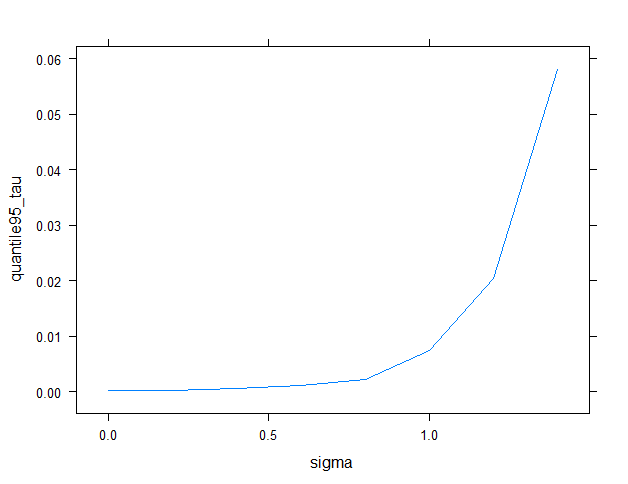
\includegraphics[width = 4.5in]{q95_tau1}
	\end{center}
	\caption{Зависимость $95\%$ квантиля для $\tau(U_1, U_2)$ от значения $\sigma$ шума.}
	\label{fig:q95_tau1}
\end{figure}

Значение $\sigma = 1$ является очень большим для рассматриваемой длины ряда, т.е. выше него шум уже сложно отличить от колебательной составляющей. Это видно по рис.~\ref{fig:q95_tau1}: после $\sigma=1$ график резко пошел вверх. Так что стоит рассматривать результаты для $\sigma=1$.

Полученные результаты говорят, что примерным необходимым значением порога является значение $t_0 = 0.01$.
Это значение было использовано при программировании для значения по умолчанию. Но эксперименты с реальными данными говорят, что оптимальное значение порога может сильно колебаться.
% но, конечно, для устойчивости значение нужно брать хотя бы в два раза большим. Для реальных данных значение можно брать еще большим, так как данные в этом случае сильнее зашумлены.

%\subsubsection{Выбор порога в случае отсутствия шума и сильной разделимости}
%Рассмотрим следующий частный случай. Пусть у рассматриваемого ряда мы смогли отделить компоненты сингулряного разложения, относящиеся к сигналу, от компонент, относящихся к шуму, и требуется с помощью полученных компонент сигнала выделить колебательную компоненту. Не гарантируется, что есть сильная разделимость среди компонент сигнала.
%
%Для борьбы с отсутствием сильной разделимости будем использовать метод\\  DerivSSA, описанный в \cite{Golyandina.Shlemov2014}, метод подходит только для ситуации, когда имеется сигнал без шума. На вход методу подаются $r$ компонент сингулярного разложения, соответствующих сигналу. DerivSSA выдает новые $r$ компонент с улучшенной сильной разделимостью. Для реализации метода использовалась функция \textsc{fossa} из пакета \textsc{Rssa} \cite{Rssa}.

%Далее из полученных $r$ компонент, в частности, из сингулярных векторов $\{U_i\}$, $i=1,\ldots,r$, отбираем компоненты, относящиеся к периодике с помощью функционала $\tau_1$. $1,\ldots,r$ --- это просто нумерация для полученных векторов, эта запись не означает, что мы берем именно первые $r$ компонент.
%
%Как обычно рассматриваем значения функционала $\tau_1(U_i, U_{i+1})$ от последовательных пар сингулярных векторов. Заметим, что к периодике не могут одновременно относится пары векторов $(U_i, U_{i+1})$ и $(U_{i+1}, U_{i+2})$. Поэтому проведем среди пар дополнительный отбор, который уменьшит количество векторов, среди которых ищем периодику. Последовательно из каждых двух пар будем выбирать ту, для которой значение функционала $\tau_1$ наименьшее. В итоге получим $s$, $s \leqslant r$, сингулярных векторов. Сортируем полученные значения функционала $\tau_1$, обозначим их тоже как  $\tau_1(U_i, U_{i+1})$, $i=1,\ldots,s$.
%
%Далее рассматриваем последовательные разности $d_i = \tau_1(U_{i+1}, U_{i+2}) - \tau_1(U_i, U_{i+1})$, $i=1,\ldots,s-1$ (будем называть их зазорами) между отсортированными значениями $\tau_1(U_i, U_{i+1})$. Выбираем значение порога между значениями $\tau_1(U_i, U_{i+1})$ и $\tau_1(U_{i+1}, U_{i+2})$, для которых $d_i$ максимально. Если все $d_i$ малы, порог выбирается большим $\tau_1(U_{s-1}, U_s)$. Для определения того мал ли зазор зададим значение $\varepsilon$. Если $\max(d_i) < \varepsilon$, то все рассматриваемые компоненты относим к периодике и выбираем порог, большим $\tau_1(U_{s-1}, U_s)$. Предлагается брать $\varepsilon = 0.01$.
%
%Приведем теперь короткий и формальный план описанного алгоритма.
%На вход поступает $r$ компонент сингулярного разложения, соответствующие сигналу, и значение $\varepsilon$.
%
%\begin{enumerate}
%\item Применяем DerivSSA, получаем новые $r$ компонент и векторы $\{U_i\}$, $i=1,\ldots,r$.
%\item Делаем отбор среди пар $(U_i, U_{i+1})$, $i=1,\ldots,r$, выбирая из двух соседних пар пару с минимальной значением $\tau_1(U_i, U_{i+1})$. Получим $s$, $s \leqslant r$, компонент. Обозначим новые вектора тоже как $\{U_i\}$, $i=1,\ldots,s$. Сортируем значения функционала и обозначим их как $\tau_1(U_i, U_{i+1})$, $i=1,\ldots,s$.
%\item Рассматриваем разности (зазоры) $d_i = \tau_1(U_{i+1}, U_{i+2}) - \tau_1(U_i, U_{i+1})$, $i=1,\ldots,s-1$.
%Если $\max(d_i) < \varepsilon$, то порог выбирается большим $\tau_1(U_{s-1}, U_s)$, иначе в качестве порога выбирается $\max(d_i)$.
%\end{enumerate}


%\subsubsection{Пример}
%Рассмотрим ряд $F_N = T_N + S_N^{(1)}+S_N^{(2)} + S_N^{(3)} + R_N$ с
%\begin{eqnarray*}
%t_k  &=& e^{0.02k}, \\
%s_k^{(1)} &=& e^{0.01k}\cos(2\pi k/10), \\
%s_k^{(2)} &=& e^{0.01k}\cos(2\pi k/15) , \\
%s_k^{(3)} &=& e^{0.01k}\cos(2\pi k/30) , \\
%r_k &=&  e^{0.01k}\sigma \varepsilon_k,
%\end{eqnarray*}
%где $\varepsilon_k$ --- независимые реализации стандартного нормального распределения $N(0,1)$, $1 \le k \le N$, $N = 199$, $\sigma = 0.8$.
%Здесь $T_N$ --- экспоненциальный тренд рагна $1$; $S_N^{(1)}$, $S_N^{(2)}$, $S_N^{(3)}$ --- э.-м. гармоники с рангом $2$, не являющиеся сильно разделимыми, т.к. имеют одинаковые амплитуды; $R_N$ --- шум.
%Возьмем длину окна $L=100$. Тогда $K=100$ тоже. Периодика --- это $S_N^{(1)}+S_N^{(2)}+S_N^{(3)}$.
%
%Предположим, мы знаем, что первые $7$ (1 комопнента тренда и 6 компонент периодики) компонент сингулярного разложения относятся к сигналу. Применим к этим компонентам алгоритм DerivSSA. На рис.~\ref{fig:fossa_wcor} изображены матрицы взвешанных корреляций до DerivSSA (слева) и после (справа). Чем темнее цвет квадрата, тем выше корреляция между компонентами, белый цвет соответствует нулевой корреляции. Видим, что алгоритм хорошо сработал, до него компоненты периодики (с первой по шестую) смешивались, а после алгоритма они (компоненты со второй по седьмую) стали сильно разделимыми.
%Заметим, что после DerivSSA компонента, соответствующая тренду, стала седьмой, а не первой.
%
%\begin{figure}[!hhh]
%	\begin{center}
%	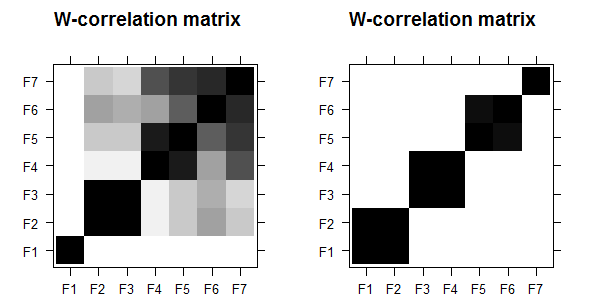
\includegraphics[width = 4in]{fossa_wcor}
%	\end{center}
%	\caption{Матрицы взвешанных корреляций до DerivSSA (слева) и после (справа).}
%	\label{fig:fossa_wcor}
%\end{figure}
%
%Далее применяем опиcанную процедуру с $\tau_1$. Отбор пар векторов выдал три пары индексов: 2 и 3, 4 и 5, 6 и 7.  Значения зазора между ними следующие: 0.0010 0.0013. Оба значения меньше чем $\varepsilon = 0.01$. Поэтому все получившиеся пары относим к периодике. Алгоритм выделения периодики сработал верно.

\chapter{Обобщения методов автоматической идентификации для разных вариантов SSA}
\label{sec:all_methods}

В данной главе приведем обобщения некоторых методов из глав \ref{sec:1d_methods} и \ref{sec:tau1} для других типов объекта $\mathbb{X}$ и вариантов метода SSA. Приведены те обобщения, которые получились и  показались разумными.

Сначала будет описано обобщение кластерного метода группировки из раздела \ref{sec:1D_wcor}, реализуемого алгоритмом \ref{alg:wcor}, сразу для всех вариантов SSA.
Затем отдельно для CSSA будет приведено обобщение метода низких частот из раздела \ref{sec:1d_freq_method}, парного частотного метода для колебательной компоненты из раздела \ref{sec:1d_pgram_method} и метода идентификации колебательной компоненты по регулярности углов из главы \ref{sec:tau1}.
Только первые два метода будут также обобщены для MSSA, и для 2S-SSA обобщим только метод низких частот.

\section{Кластерный метод группировки}
В разделе \ref{sec:sep} приведены общие для всех типов объекта $\mathbb{X}$ определения w-корреляции и матрицы w-корреляций. Поэтому кластерный метод группировки и его алгоритм \ref{alg:wcor}, приведенные в разделе \ref{sec:1D_wcor}, одинаковы для всех типов объекта $\mathbb{X}$.

\section{Обобщения для CSSA}
Рассматриваем комплекснозначный временной ряд длины $N$: $\mathbb{X}=\mathbb{X}^{(1)} + \I \,\mathbb{X}^{(2)}$, $\mathbb{X}^{(k)}= \left(x^{(k)}(1),\ldots,x^{(k)}(N)\right)$, $k=1,2$, $x^{(k)}(i) \in \mathsf{R}$.

Комплексные временные ряды --- это искусственная вещь, в реальных задачах такие почти не встречается, за исключением комплексной экспоненты, т.е. э-м гармоники \eqref{eq:complex_exmodgarm} c $a=b$ и $|\phi_1 - \phi_2| = \pi/2 \,\,(\mod \pi)$. Пример, в котором возникают комплексные экспоненты, будет приведен далее в разделе \ref{sec:use_cssa}.

Таким образом, при идентификации комплексной колебательной составляющей наша главная цель --- идентифицировать гармоники ранга 1 с $a=b$ и $|\phi_1 - \phi_2| = \pi/2 \,\,(\mod \pi)$.
Парный частотный метод будет обобщен именно для этого случая. Для метода по регулярности углов также приведем обобщение для э-м гармоник ранга 2 с $\omega \not = 0.5$, как говорилось в главе \ref{sec:tau1}, для $\omega=0.5$ метод по регулярности углов не работает. 

%\subsection{Кластерный метод группировки} \label{sec:cssa_wcor}
%Для комплексного ряда $\mathbb{X}$ аналогично 1D-SSA вводится определение \eqref{eq:w_i} w-корреляции и определение \eqref{eq:1d_w_scalar_prod} скалярного произведения  $\left(\mathbb{X}_1, \mathbb{X}_2 \right)_w$ для двух комплексных рядов  $\mathbb{X}_1$ и $\mathbb{X}_2$. Сам метод полностью аналогичен кластерному методу для  1D-SSA, реализуемому алгоритмом \ref{alg:wcor}.
%

\subsection{Метод низких частот для идентификации тренда}
\label{sec:freq_method_cssa}
Обобщим алгоритм \ref{alg:freq1d} идентификации тренда из раздела \ref{sec:1d_freq_method} на случай комплексного ряда. Алгоритм \ref{alg:freq1d} можно было применять либо к левым или правым сингулярным векторам, либо к восстановленным рядам.

%Из утверждения \ref{th:cssa_ex_mod_im_vec} мы знаем, что в CSSA левые и правые сингулярные вектора являются комплексными временными рядами, также они имеют примерно такой же вид, что и исходный ряд, которому они соответствуют.

Из общего вида алгоритма SSA, описанного  разделе \ref{sec:ssa_alg}, видим, что в CSSA и левые и правые сингулярные вектора и восстановленные ряды являются комплексными, значит, к ним можно применять алгоритм равнозначно.

Предлагается алгоритм \ref{alg:freqcssa}, похожий на частотный алгоритм \ref{alg:freq1d} для 1D-SSA, но в котором в отличие от алгоритма \ref{alg:freq1d} на первом шаге будем вычислять меру отдельно для мнимой и вещественной частей $\mathbb{Y}_i$ и брать из них максимальную для использования на 2 шаге алгоритма. 
Берется именно максимум, а не, например, среднее, потому что если для какой-то компоненты $\mathbb{Y}_i$, вещественная часть, соответствующая ряду $\mathbb{S}_1$, относится к тренду, а мнимая часть, соответствующая ряду $\mathbb{S}_2$, не относится, то среднее дало бы маленькое значение меры, которое могло бы не превзойти порог $T_0$.
%Таким образом, если хотя бы для одной исходной составляющей компонента $\mathbb{Y}_i$ относится к тренду, то мы её выделим. 

\begin{algorithm}[!hhh]
\caption{CSSA. Метод низких частот для тренда}
\label{alg:freqcssa}
\begin{algorithmic}[1]
\REQUIRE Значение  $0 \leqslant  \omega \leqslant 0.5$, порог $0 \leqslant T_0 \leqslant 1$, группа индексов $I$, тип рядов $\mathbb{Y}_i$,\\ $i \in I$: левые сингулярные вектора,
правые сингулярные вектора или восстановленные ряды.
\ENSURE Группа индексов компонент $J \subset I$.
\STATE  Для каждого ряда $\mathbb{Y}_i = \mathbb{Y}^{(1)}_i + \I \mathbb{Y}^{(2)}_i $, $i \in I$, вычисляем значения $T(\mathbb{Y}^{(1)}_i; \omega)$ и $T(\mathbb{Y}^{(2)}_i; \omega)$ с помощью \eqref{eq:T_measure}. $T_m := \max \{T(\mathbb{Y}^{(1)}_i; \omega); T(\mathbb{Y}^{(2)}_i; \omega)\}$.
\STATE $J$ --- группа индексов $i \in I$, таких что $T_m \geqslant T_0$.
\end{algorithmic}
\end{algorithm}

\subsection{Парный частотный метод идентификации колебательной компоненты}
Как мы знаем, колебательная составляющая является суммой э-м гармоник.
Согласно разделу \ref{sec:cssa_theory} главы \ref{sec:ssa_theory} элементы комплекснозначного э.-м. гармонического ряда $\mathbb{S}$ имеют вид \eqref{eq:complex_exmodgarm}.
%\begin{equation*} 
% s(n) = e^{\alpha n} (a\cos(2\pi\omega n + \phi_1) + \I \,b\cos(2\pi\omega n + \phi_2)),
%\end{equation*}
%где $0 \leqslant\phi_1, \phi_2 < 2\pi$, $a, b \not = 0$, $0<\omega \leqslant 0.5$, $\sin \phi_1 \not = 0$ или $\sin \phi_2 \not = 0$ для $\omega = 0.5$.

Из утверждения \ref{th:cssa_ex_mod_im_vec} известно, для ряда $\mathbb{S}$ ранг ряда $d$ может равняться или $2$, или $1$, т.е. ему может соответствовать либо один, либо два левых сингулярных вектора. 

\begin{remark}
По утверждению \ref{th:cssa_num} собственные числа комплексной э-м гармоники не являются равными, поэтому в случае CSSA, чтобы найти пары сингулярных векторов, соответствующие гармонике ранга 2, недостаточно рассматривать последовательные пары, нужно рассматривать всевозможные пары векторов.
\end{remark}

Как уже отмечали в начале раздела, будем идентифицировать гармоники $\mathbb{S}$ ранга 1 c $a=b$ и $|\phi_1 - \phi_2| = \pi/2 \,\,(\mod \pi)$.
%Будем идентифицировать гармоники ранга 1 и ранга 2 одновременно. 
%\ref{sec:cssa_theory} из утверждения \ref{th:cssa_ex_mod_im_vec} этого же раздела следует, что если $\omega$ и $\phi_j$ такие, что $d = 2$, то элементы сингулярных векторов $U_1$ и $U_2$ ряда $\mathbb{S}$ можно представить в  виде \eqref{eq:uuu1} и \eqref{eq:uuu2} соответственно.
%Мнимая и вещественная части векторов имеют одинаковую частоту.
 Из утверждения \ref{th:cssa_ex_mod_im_vec} раздела \ref{sec:cssa_theory} следует, что в случае $a=b$ и $|\phi_1 - \phi_2| = \pi/2 \,\,(\mod \pi)$ единственный сингулярный вектор $U_1$ ряда $\mathbb{S}$ имеет вид \eqref{eq:vid_d1}, это сумма синуса и косинуса с одинаковой частотой $\omega$.

Парный частотный метод для 1D-SSA имел два этапа, на каждом этапе сингулярный вектор $U_j$ участвовал только в значении его периодограммы $\Pi_{U_j}^L(k/L)$.

Ввиду сказанного алгоритм идентификации комплексной э-м гармоники следующий. Применяем алгоритм, как для 1D-SSA только вместо последовательной пары $U_i, U_{i+1}$ сингулярных векторов берем пару векторов, соответствующих мнимой и вещественной части  комплексного вектора $U_i$, нормированных на свою длину, так как для метода важно чтобы вектора имели норму 1. 
Таким образом введем следующие обозначения.  
\begin{gather} \label{eq:I_1_P_cssa}
I_1^{(\mathbb{P})} = \{ i: \quad \theta_1 \theta_2 >0, \quad L |\theta_i - \theta_{i+1}| \leqslant s_0, \quad 1 \leqslant i \leqslant L -1  \},
\end{gather}
где $\theta_i = \argmax_{0 < k \leqslant L/2} \{\Pi_{\RE(U_i)}^L(k/L)\}$, $\theta_{i+1} = \argmax_{0 < k \leqslant L/2} \{\Pi_{\IM(U_i)}^L(k/L)\}$ --- аргументы максимума периодограмм $\Pi_{\RE(U_i)}^L$ и $\Pi_{\IM(U_i)}^L$ вещественной и мнимой частей сингулярного вектора $U_i$ соответственно.
\begin{gather*}
\rho_{i} := \max_{0 \leqslant k \leqslant L/2}{\left(\rho_{\{\RE(U_i),\IM(U_i)\}}(k/L) + \rho_{\{\RE(U_i),\IM(U_i)\}}((k+1)/L)\right)},
\end{gather*}
определение \ref{def:rho} меры $\rho_A$ дано в разделе \ref{sec:1d_pgram_method}.
\begin{gather} \label{eq:pgram_I_p_cssa}
I^{(\mathbb{P})} = \{ i \in I_1^{(\mathbb{P})}: \rho_{i} \geqslant\rho_0 \}.
\end{gather}
Ниже приведем алгоритм \ref{alg:cssa_pgram} парного частотного метода для CSSA.
\begin{algorithm}[!hhh]
\caption{СSSA. Парный частотный метод для колебательной составляющей}
\label{alg:cssa_pgram}
\begin{algorithmic}[1]
\REQUIRE Параметр $s_0 \in \mathsf{Z}_{+}$, порог $\rho_0 \in [0,1]$.
\ENSURE Номера индексов сингулярных векторов $I^{(\mathbb{P})}$, относящихся к колебательной составляющей.
\STATE  Получаем группу индексов $I_1^{(\mathbb{P})}$ с помощью $s_0$ и \eqref{eq:I_1_P_cssa}.
\STATE Получаем группу $I^{(\mathbb{P})}$ по $\{U_j\}_{j \in I_1^{(\mathbb{P})}}$ и $\rho_0$ с помощью \eqref{eq:pgram_I_p_cssa}.
\end{algorithmic}
\end{algorithm}


%Таким образом, если какие-то два ряда имеют колебательные компоненты с одинаковой частотой, то CSSA и предложенный алгоритм позволят их выделить. Если же колебательные компоненты рядов имеют разные частоты или нет никаких предположений об их частотах, то лучше исследовать каждый ряд с помощью 1D-SSA. 
\newpage
\subsection{Метод идентификации колебательной компоненты по регулярности углов}
\label{sec:tau_cssa}
Как уже отмечалось ранее в начале раздела про обобщения CSSA и в главе \ref{sec:tau1} для данного метода мы не рассматриваем случай $\omega=0.5$.

Описание метода идентификации колебательной компоненты по регулярности углов из главы \ref{sec:tau1} для комплексных э-м гармоник, основанного на специальной мере $\tau$, задаваемой формулой \eqref{eq:tau1}, было приведено в бакалаврской работе \cite{Zhornikova2016}. Опишем метод и приведем этот алгоритм.

Для $d=2$ вид левых сингулярных векторов для комплексной гармоники приведен в формулах \ref{eq:uuu1} и \eqref{eq:uuu2} в разделе \eqref{sec:cssa_theory}.
Из утверждения \ref{th:th_tau_cssa} этого же раздела следует, что при определенных условиях всегда существует один поворот $2\pi t$ или последовательность поворотов $2\pi t = 2\pi t_L$ и для мнимой и для вещественной частей вектора $U_2$, приводящий к равенствам
\begin{gather*}
\lim_{L \rightarrow \infty}(\tau (\RE U_1, \RE e^{\I 2\pi t} U_2) + \tau (\IM U_1, \IM e^{\I 2\pi t} U_2))= 0.
\end{gather*}
Поэтому для случая $d=2$ для пары $(U_i,\,U_j)$, $i<j$, решается оптимизационная задача
\begin{gather} \label{eq:cssa_tau_opt}
 \tau(\RE U_i, \RE e^{\I 2\pi t} U_j) + \tau(\IM U_i, \IM e^{\I 2\pi t} U_j) \longrightarrow \min_{t}.
\end{gather}
На $t_{i,j}$ достигается минимум, $\tau_{i,j}$ --- минимальное значение.
Отбираем пары индексов $i$, $j$ векторов $\left(U_i, \,\,e^{\mathrm{i} 2\pi t_{i,j}}U_j\right)$, у которых значение меры $\tau_{i,j}$
меньше заданного порога $t_0$, или берем фиксированное число э-м гармоник, если оно задано, с наименьшими значениями $\tau_{i,j}$.

Для $d=1$ единственный сингулярный вектор имеет вид \eqref{eq:vid_d1} и, согласно  утверждению \ref{th:th_tau_cssa_d1} раздела \ref{sec:cssa_theory} рассматриваем значения $\tau(\RE U_i, \IM U_i)$.
Отбираем индексы $i$ векторов $U_i$, у которых значение меры $\tau(\RE U_i, \IM U_i)$
меньше заданного порога $t_0$,
или берем фиксированное число э-м гармоник, если оно задано, с наименьшими значениями $\tau(\RE U_i, \IM U_i)$.

Как и в вещественном случае метод имеет две модификации. Для случая, когда число комплексных э-м гармоник известно, метод реализуется алгоритмом \ref{alg:cssatau_2}, для случая с неизвестным числом комплексных э-м гармоник --- алгоритмом \ref{alg:cssatau}. 

\begin{algorithm}[!hhh]
\caption{CSSA. Метод по регулярности углов для колебательной составляющей, число э-м гармоник известно}
\label{alg:cssatau_2}
\begin{algorithmic}[1]
\REQUIRE Количество $m_1$ э-м гармоник ранга 1 и количество $m_2$ э-м гармоник ранга 2,  $m_1, m_2 \leqslant d$.
\ENSURE Группа индексов компонент $J$.
\STATE Для пары $(U_i,\,U_j)$, $i<j$, решается оптимизационная задача \eqref{eq:cssa_tau_opt}.
На $t_{i,j}$ достигается минимум, $\tau_{i,j}$ --- минимальное значение;\\
$\tau_1^{(1)}, \ldots, \tau_d^{(1)}$ --- отсортированные значения $\tau(\RE U_j, \IM U_j)$, $j=1,\ldots, d$;\\
$\tau_1^{(2)}, \ldots, \tau_{d(d-1)}^{(2)}$ --- отсортированные значения $\tau_{i,j}$, $i,j=1,\ldots, d$, $i \not = j$.
\STATE  $J_1$ --- индексы $j$ сингулярных векторов $U_j$, участвующих в вычислении\\ $\tau_1^{(1)}, \ldots, \tau_{m_1}^{(1)}$.
\STATE  $J_2$ --- индексы $i$, $j$ сингулярных векторов $U_i$ и $U_j$, участвующих в вычислении $\tau_1^{(2)}, \ldots, \tau_{m_2}^{(2)}$ .
\STATE $J = J_1 \cup J_2$.
\end{algorithmic}
\end{algorithm}

\begin{algorithm}[!hhh]
\caption{CSSA. Метод по регулярности углов для колебательной составляющей, число э-м гармоник неизвестно}
\label{alg:cssatau}
\begin{algorithmic}[1]
\REQUIRE Порог $t_0 \geqslant 0$.
\ENSURE Группа индексов компонент $J$.
\STATE Для пары $(U_i,\,U_j)$, $i<j$, решается оптимизационная задача \eqref{eq:cssa_tau_opt}.
На $t_{i,j}$ достигается минимум, $\tau_{i,j}$ --- минимальное значение.
\STATE  $J_1$ --- индексы сингулярных векторов $U_j$, для которых $\tau(\RE U_j, \IM U_j) < t_0$.
\STATE  $J_2$ --- индексы векторов  $U_i$, $U_j$, для которых  $\tau_{i,j} < t_0$.
\STATE $J = J_1 \cup J_2$.
\end{algorithmic}
\end{algorithm}

Проблемы выбора порога в комплексном случае аналогичны случаю 1D-SSA.
(Но можно дать рекомендации по модельным данным --- это надо сделать).

\section{Обобщения для MSSA}

Рассматриваем многомерный временной ряд $\mathbb{X}= \left(\mathbb{X}^{(1)}, \ldots,\mathbb{X}^{(s)}\right)$,\\ $\mathbb{X}^{(p)}= \left(x^{(p)}(1),\ldots,x^{(p)}(N_p)\right)$, $p=1,\ldots,s$, $x^{(p)}(i) \in \mathsf{R}$. 

Основная особенность MSSA, в отличие от вещественного или комплексного случая, состоит в том, что все три вида объектов: восстановленные ряды, левые сингулярные вектора и правые сингулярные вектора, имеют разную структуру.

Из описания алгоритма MSSA, приведенного в разделе \ref{sec:ssa_alg}, следует, что восстановленные ряды имеют такое же вид, как и исходный многомерный ряд, т.е. тоже являются многомерными рядами (или системой временных рядов). 

Из утверждения \ref{th:mssa_vec} для MSSA левые сингулярные вектора --- это одномерные вещественнозначные временные ряды
 длины $L$, каждый левый сингулярный вектор состоят из элементов одного из рядов $\mathbb{X}^{(1)}, \ldots, \mathbb{X}^{(s)}$. 
 
 Правые сингулярные вектора также являются одномерными вещественнозначными временными рядами длины $L$, но состоят из 
последовательных частей каждого из рядов $\mathbb{X}^{(1)}, \ldots, \mathbb{X}^{(s)}$.
Введем для правых сингулярных векторов следующие обозначения: 
\begin{gather} \label{eq:V_mssa}
{V}_{i} = \left({V}_i^{(1)}, \ldots, {V}_i^{(s)}\right), 
\end{gather}
где $V_i^{(1)}$ --- первые $K_1$ элементов вектора ${V}_{i}$,  $V_i^{(2)}$, --- вторые $K_2$ элементов вектора ${V}_{i}$ и, так далее, $V_i^{(s)}$ --- последние $K_s$ элементов вектора ${V}_{i}$, $0 \leqslant i \leqslant d$. 

Ввиду сказанного, для MSSA алгоритмы будут иметь разные модификации для разных вариантов входных объектов. Разные модификации алгоритмов могут давать разные результаты, например, в случае применения алгоритма к правым сингулярным векторам, в отличие от левых сингулярных векторов, в каждом векторе учитывается каждый из $s$ рядов.  
 
%\subsection{Кластерный метод группировки} \label{sec:mssa_wcor}
%Для обобщения метода из раздела \ref{sec:1D_wcor} нужно только ввести определения
%w-корреляции и скалярного произведения  $\left(\mathbb{X}_1, \mathbb{X}_2 \right)_w$ двух многомерных рядов  $\mathbb{X}_1$ и $\mathbb{X}_2$.
%
%Пусть, как и ранее, $L^* = \min(L,K)$ и $K^* = \max(L,K)$. Зададим веса
%\begin{gather*}
% w^{(p)}(i) =
%\begin{cases}
%i &\quad \text{для } 0 \leqslant i \leqslant L^*, \\
%L^* & \quad \text{для } L^* \leqslant i \leqslant K^*, \\
%N_p - i + 1 & \quad \text{для } K^* \leqslant i \leqslant N_p.
%\end{cases}
%\end{gather*}
%
%Определим скалярное произведение $\left(\mathbb{X}_1, \mathbb{X}_2 \right)_w$ двух многомерных рядов  $\mathbb{X}_1$ и $\mathbb{X}_2$.
% \begin{equation*}
%\left(\mathbb{X}_1, \mathbb{X}_2 \right)_w = \sum_{p=1}^{s} \sum_{i=1}^{N_p}w^{(p)}(i) x_1^{(p)}(i) x_2^{(p)}(i).
%\end{equation*}

\subsection{Метод низких частот для идентификации тренда}
\label{sec:freq_method_mssa}

Обобщим алгоритм \ref{alg:freq1d} идентификации тренда из раздела \ref{sec:1d_freq_method} на случай многомерного ряда. Алгоритм \ref{alg:freq1d} можно было применять либо к левым или правым сингулярным векторам, либо к восстановленным рядам. 

Как уже говорилось, в MSSA левые сингулярные вектора являются одномерными вещественнозначными временными рядами длины $L$ и состоят из элементов одного из рядов $\mathbb{X}^{(1)}, \ldots, \mathbb{X}^{(s)}$. Т.е. левые сингулярные вектора имеют такой же вид, как в случае 1D-SSA, к ним можно применить частотный алгоритм \ref{alg:freq1d} точно так же. Алгоритм \ref{alg:freqmssa_1} для этого случая приведен ниже.

Правые сингулярные вектора также являются одномерными вещественнозначными временными рядами длины $L$, но состоят из последовательных частей каждого из рядов $\mathbb{X}^{(1)}, \ldots, \mathbb{X}^{(s)}$ и представимы в виде \eqref{eq:V_mssa}. К частям ${V}_i^{(1)}, \ldots, {V}_i^{(s)}$ правого сингулярного вектора $V_i$ мы можем применить метод низких частот, аналогично, как в комплексном случае применяли в мнимой и вещественной части вектора: считаем меру \eqref{eq:T_measure} для каждой части ${V}_i^{(1)}, \ldots, {V}_i^{(s)}$ вектора $V_i$, и берем максимум. Предлагаемый алгоритм \ref{alg:freqmssa_2} формально описан ниже.

Восстановленные ряды в случае MSSA являются также многомерными временными рядами, идея применения такая же, как в комплексном случае или для правых сингулярных векторов: на первом шаге для каждого из $s$ рядов считаем меру по формуле \eqref{eq:T_measure} и берем максимальное значение этой меры для использования на втором шаге.
Этот вариант метода задается алгоритмом  \ref{alg:freqmssa_3}.

 \begin{algorithm}[!hhh]
\caption{MSSA. Метод низких частот для тренда: вариант с левыми сингулярными векторами}
\label{alg:freqmssa_1}
\begin{algorithmic}[1]
\REQUIRE Значение  $0 \leqslant  \omega \leqslant 0.5$, порог $0 \leqslant T_0 \leqslant 1$, группа индексов $I$, левые сингулярные вектора $U_i$, $i \in I$.
\ENSURE Группа индексов компонент $J \subset I$.
\STATE  Для каждого вектора $U_i$, $i \in I$, вычисляем значение $T(U_i; \omega)$ с помощью  \eqref{eq:T_measure}.
\STATE $J$ --- группа индексов $i \in I$, таких что $T(U_i; \omega) \geqslant T_0$
\end{algorithmic}
\end{algorithm}

\begin{algorithm}[!hhh]
\caption{MSSA. Метод низких частот для тренда: вариант с правыми сингулярными векторами}
\label{alg:freqmssa_2}
\begin{algorithmic}[1]
\REQUIRE Значение  $0 \leqslant  \omega \leqslant 0.5$, порог $0 \leqslant T_0 \leqslant 1$, группа индексов $I$,
правые сингулярные вектора $V_i$, $i \in I$.
\ENSURE Группа индексов компонент $J \subset I$.
\STATE  Для каждого вектора ${V}_{i} = ({V}_i^{(1)}, \ldots,{V}_i^{(s)})$, $i \in I$
 вычисляем значения $T(V_i^{(1)}; \omega), \ldots,
T(V_i^{(s)}; \omega)$ с помощью  \eqref{eq:T_measure}. $T_m := \max \{T(V_i^{(1)}; \omega); \ldots;
T(V_i^{(s)}; \omega)\}$.
\STATE $J$ --- группа индексов $i \in I$, таких что $T_m \geqslant T_0$.
\end{algorithmic}
\end{algorithm}

\begin{algorithm}[!hhh]
\caption{MSSA. Метод низких частот для тренда: вариант с восстановленными рядами}
\label{alg:freqmssa_3}
\begin{algorithmic}[1]
\REQUIRE Значение  $0 \leqslant  \omega \leqslant 0.5$, порог $0 \leqslant T_0 \leqslant 1$, группа индексов $I$,
восстановленные ряды $\mathbb{Y}_{i}$, $i \in I$.
\ENSURE Группа индексов компонент $J \subset I$.
\STATE  Для каждого ряда $\mathbb{Y}_{i} = (\mathbb{Y}_i^{(1)}, \ldots, \mathbb{Y}_i^{(s)})$, $i \in I$, вычисляем значения $T(\mathbb{Y}_i^{(1)}; \omega), \ldots,
T(\mathbb{Y}_i^{(s)}; \omega)$ с помощью  \eqref{eq:T_measure}. $T_m := \max \{T(\mathbb{Y}_i^{(1)}; \omega); \ldots;
T(\mathbb{Y}_i^{(s)}; \omega)\}$.
\STATE $J$ --- группа индексов $i \in I$, таких что $T_m \geqslant T_0$.
\end{algorithmic}
\end{algorithm}

\newpage
\subsection{Парный частотный метод идентификации колебательной компоненты}
Колебательная составляющая является суммой э-м гармоник.
Согласно разделу \ref{sec:mssa_theory} элементы многомерного э.-м. гармонического ряда $\mathbb{S}$ имеют вид \eqref{eq:em_mssa}.

%Из утверждения \ref{th:cssa_ex_mod_im_vec} известно, для ряда $\mathbb{S}$ ранг ряда $d$ может равняться или $2$, или $1$, т.е. ему может соответствовать либо один, либо два левых сингулярных вектора. 
%
%\begin{remark}
%По утверждению \ref{th:cssa_num} собственные числа комплексной э-м гармоники не являются равными, поэтому в случае CSSA, чтобы найти пары сингулярных векторов, соответствующие гармонике ранга 2, недостаточно рассматривать последовательные пары, нужно рассматривать всевозможные пары векторов.
%\end{remark}
%
%
%Элементы одномерной вещественной э-м гармоники $\mathbb{S}$ имеют вид
%\begin{equation*}
% s(n) = e^{\alpha n} a\cos(2\pi\omega n + \phi),
%\end{equation*}
%где $0 \leqslant \phi < 2\pi$, $a \not = 0$, $0<\omega \leqslant 0.5$, $\sin \phi \not = 0$ для $\omega = 0.5$.
%В многомерном случае мы имеем несколько таких рядов, возможно, с разными частотами.

Как уже упоминалась в предыдущем разделе, по утверждению \ref{th:mssa_vec} в MSSA левые сингулярные вектора являются одномерными вещественнозначными временными рядами длины $L$, и каждый левый сингулярный вектор состоит из элементов одного из 
рядов $\mathbb{X}^{(1)}, \ldots, \mathbb{X}^{(s)}$. Поэтому к ним парный частотный метод можно применить точно так же, как в случае 1D-SSA. Ниже приведем алгоритм \ref{alg:mssa_pgram_1} парного частотного метода для MSSA и левых сингулярных векторов.

\begin{algorithm}[!hhh]
\caption{MSSA. Парный частотный метод для колебательной составляющей: вариант с левыми сингулярными векторами}
\label{alg:mssa_pgram_1}
\begin{algorithmic}[1]
\REQUIRE Параметр $s_0 \in \mathsf{Z}_{+}$, порог $\rho_0 \in [0,1]$.
\ENSURE Группа индексов компонент $I^{(\mathbb{P})}$.
\STATE  Получаем группу индексов $I_1^{(\mathbb{P})}$ с помощью $s_0$ и \eqref{eq:I_1_P} и группу индексов $I_2^{(\mathbb{P})}$ с помощью \eqref{eq:I_2_P}.
\STATE Получаем группу $I^{(\mathbb{P})}$ по $\rho_0$ и $\{U_j\}_{j \in I_1^{(\mathbb{P})} \cup I_2^{(\mathbb{P})}}$ с помощью  \eqref{eq:pgram_I_p}.
\end{algorithmic}
\end{algorithm}

Правые сингулярные вектора
%также являются одномерными вещественнозначными временными рядами длины $L$ и
состоят из последовательных частей длины $K_1,\ldots,K_s$ каждого из рядов $\mathbb{X}^{(1)}, \ldots, \mathbb{X}^{(s)}$ и имеют вид \eqref{eq:V_mssa}.

Так как вектора, в которым применяем парный частотный метод, должны иметь норму 1, то вместе векторов $V_i$ рассмотрим вектора: 
\begin{gather*}
\widehat{V}_{i} := \left(\widehat{V}_i^{(1)}, \ldots, \widehat{V}_i^{(s)}\right),
\end{gather*}
где
\begin{gather*} \label{eq:V_norm_mssa}
\widehat{V}_i^{(p)} := \frac{V_i^{(p)}}{\|V_i^{(p)} \|},
\end{gather*}
т.е $\| \widehat{V}_i^{(p)} \| = 1$. 

%Если многомерный ряд имеет размерность $s=2$, то к правым сингулярным векторам парный частотный метод можно применить почти также как к комплексным сингулярным векторам: применяем алгоритм, как для 1D-SSA только вместо последовательной пары $U_i, U_{i+1}$ сингулярных векторов берем в качестве пары векторов первые $K$ элементов правого сингулярного вектора и вторые $K$ элементов.
%Введем обозначения для правых сингулярных векторов:
%\begin{gather*}
%{V}_{i} = \left({V}_i^{(1)}, \ldots, {V}_i^{(s)}\right),
%\end{gather*}
%где $V_i^{(1)}$ --- первые $K_2$ элементов вектора ${V}_{i}$,  $V_i^{(2)}$, --- вторые $K_2$ элементов вектора ${V}_{i}$ и так далее, $V_i^{(s)}$ --- последние $K_s$ элементов вектора ${V}_{i}$, $0 \leqslant i \leqslant d$.
%Вектора $V_i^{(p)}$ были нормированы так, чтобы иметь норму 1.
%

На первом этапе метода будет обирать множества индексов $I_{1,p}^{(\mathbb{P})}$, $p=1,\ldots,s$:
\begin{gather} \label{eq:I_1_P_mssa}
I_{1,p}^{(\mathbb{P})} = \{ i: \quad \theta_{i}^{(p)} \theta_{i+1} ^{(p)} >0, \quad L |\theta_i^{(p)} - \theta_{i+1}^{(p)}| \leqslant s_0, \quad 1 \leqslant i \leqslant K -1  \},
\end{gather}
где $\theta_i^{(p)} = \argmax_{0 < k \leqslant L/2} \{\Pi_{\widehat{V}_i^{(p)}}^L(k/L)\}$, $p=1,\ldots,s$.
Т.е. 
%для правых сингулярных векторов $\widehat{V}_i$, $\widehat{V}_{i+1}$ длины $K$
мы последовательно вычисляем множества $I_{1,p}^{(\mathbb{P})}$ для каждой пары векторов  $\widehat{V}_i^{(p)}$, $\widehat{V}_{i+1}^{(p)}$ длины $K_p$.

Аналогично каждый сингулярный вектор проверяется на соответствие гармонике с периодом 2:
\begin{gather} \label{eq:I_2_P_mssa}
I_{2,p}^{(\mathbb{P})} = \{i: \quad  L |\theta_{i}^{(p)} - 0.5 | \leqslant s_0, \quad 1 \leqslant i \leqslant K  \}.
\end{gather}

Далее для второго этапа введем определение
\begin{gather*}
\rho_{i,j} :=  \max_p \{ \max_{0 \leqslant k \leqslant L/2}{\left(\rho_{\{\widehat{V}_i^{(p)}, \widehat{V}_{j}^{(p)}\}}(k/L) + \rho_{\{\{\widehat{V}_i^{(p)}, \widehat{V}_{j}^{(p)}\}}((k+1)/L)\right)}, p=1,\ldots, s
 \},
\end{gather*}
где $\widehat{V}_i^{(p)}, \widehat{V}_{j}^{(p)}$ --- вектора с индексами из множества индексов $I_{1,p}^{(\mathbb{P})}$ отобранных на первом этапе,
определение \ref{def:rho} меры $\rho_A$ дано в разделе \ref{sec:1d_pgram_method}.
\begin{gather} \label{eq:pgram_I_p_mssa}
I^{(\mathbb{P})} = \{ i: \rho_{i} \geqslant\rho_0 \}.
\end{gather}

Для идентификации компонент, относящихся к гармоники ранга 2, мера имеет вид
\begin{gather*}
\rho_{i} :=  \max_p \{ \max_{0 \geqslant k \geqslant L/2}{\left(\rho_{\{\widehat{V}_i^{(p)}\}}(\lfloor L/2 \rfloor/L) + \rho_{\{\{\widehat{V}_i^{(p)}\}}((\lfloor L/2 \rfloor + 1)/L)\right)}, p=1,\ldots, s
 \},
\end{gather*}
где $i \in I_{2,p}^{(\mathbb{P})}$.

Итоговым результатом парного частотного метода метода для MSSA и правых сингулярных векторов, реализуемого алгоритмом \ref{alg:mssa_pgram_2}, являются индексы 
\begin{gather} \label{eq:pgram_I_p_mssa}
I^{(\mathbb{P})} = \{ (i,j): \rho_{i,j} \geqslant\rho_0 \} \cup \{ i: \rho_{i} \geqslant\rho_0 \}.
\end{gather}

%Ниже приведем алгоритм \ref{alg:mssa_pgram_2} парного частотного метода для MSSA и правых сингулярных векторов.

\begin{algorithm}[!hhh]
\caption{MSSA. Парный частотный метод для колебательной составляющей: вариант для правых сингулярных векторов и $s=2$}
\label{alg:mssa_pgram_2}
\begin{algorithmic}[1]
\REQUIRE Параметр $s_0 \in \mathsf{Z}_{+}$, порог $\rho_0 \in [0,1]$.
\ENSURE Группа индексов компонент $I^{(\mathbb{P})}$.
\STATE  Получаем группы индексов $I_{1,p}^{(\mathbb{P})}$, $p=1,\ldots,s$, с помощью $s_0$ и \eqref{eq:I_1_P_mssa} и группы индексов $I_{2,p}^{(\mathbb{P})}$, $p=1,\ldots,s$, с помощью $s_0$ и \eqref{eq:I_2_P_mssa}.
\STATE Получаем группу $I^{(\mathbb{P})}$ с помощью $\rho_0$ и \eqref{eq:pgram_I_p_mssa}.
\end{algorithmic}
\end{algorithm}

%Таким образом, если какие-то два ряда имеют колебательные компоненты с одинаковой частотой, то MSSA и предложенный алгоритм \ref{alg:mssa_pgram_2} позволят их выделить. Если же колебательные компоненты рядов имеют разные частоты или нет никаких предположений об их частотах, то лучше использовать левые сингулярные вектора.

%\subsection{Метод идентификации колебательной компоненты по регулярности углов} 
%Опять же, если мы рассматриваем левые сингулярные вектора, то алгоритм можно применить точно так же, как в случае 1D-SSA.
%
%К правым сингулярным векторам метод не применить, потому что два случайных вектора от разных рядов никак не гарантируют свойств регулярности.

\newpage
\section{Обобщения для 2D-SSA}

Рассматриваем поле размера $N_x \times N_y$: $\mathbb{X}= \left(x(i,j) \right)_{i,j=1}^{N_x,N_y}$, $x(i,j) \in \mathsf{R}$.

Согласно разделу \ref{sec:2d_ssa_theory} главы \ref{sec:ssa_theory} элементы двумерной гармоники $\mathbb{S}$ с частотами $\omega^{(X)}$, $\omega^{(Y)}$ имеют вид:
\begin{gather} \label{eq:2d_cos_el}
\notag
s(k,l) =  \left(
\begin{matrix}
\cos(2\pi \omega^{(X)}k) \\ \notag
\sin(2\pi \omega^{(X)}k)
\end{matrix}
\right)^{\mathrm{T}}
 \left(
\begin{matrix}
a & b \\
c & d
\end{matrix}
\right)
 \left(
\begin{matrix}
\cos(2\pi \omega^{(Y)}l) \\ \notag
\sin(2\pi \omega^{(Y)}l)
\end{matrix}
\right),
\notag
\end{gather}
где $1 \leqslant k \leqslant N_x$, $1 \leqslant l \leqslant N_y$, хотя бы один коэффициент из  группы $\{a,b,c,d\}$ не равен нулю и
$\omega^{(X)}, \omega^{(Y)} \in (0,0.5)$.

Колебательная составляющая --- это сумма $\mathbb{H}$ какого-то числа $c$ двумерных гармоник. Элементы $\mathbb{H}$ имеют вид
\begin{gather} \label{eq:2d_cos}
h(k,l) = \sum_{m=1}^{c}{s_m(k,l)},
\end{gather}
где $s_m(k,l)$ --- элементы гармоники $\mathbb{S}_m$, $m=1,\ldots,c$.
\begin{gather}
\notag
h(k,l) = \sum_{m=1}^{c}(a \cos(2\pi \omega^{(X)}k) \cos(2\pi \omega^{(Y)}l) +
b_m \cos(2\pi \omega^{(X)}k) \sin(2\pi \omega^{(Y)}l) + \\ \label{eq:2d_cos_el}
c_m \sin(2\pi \omega^{(X)}k) \cos(2\pi \omega^{(Y)}l) +
d_m \sin(2\pi \omega^{(X)}k) \sin(2\pi \omega^{(Y)}l)),
\end{gather}
где $1 \leqslant k \leqslant N_x$, $1 \leqslant l \leqslant N_y$, хотя бы один коэффициент из каждой группы $\{a_m,b_m,c_m,d_m\}$ не равен нулю, а также выполняются условия
\begin{align} \label{eq:2d_omega}
\begin{matrix}
(\omega_n^{(X)}, \omega_n^{(Y)}) \not = (\omega_m^{(X)}, \omega_m^{(Y)}), \quad \text{для } n \not= m,\\
\omega_m^{(X)}, \omega_m^{(Y)} \in (0,0.5).
\end{matrix}
\end{align}

Из утверждения \ref{th:2d_rank_cos} следует, что ранг $\nu_m$ одной гармоники $\mathbb{S}_m$ равен либо 2, либо 4. Ранг равен 2, когда $a_m = d_m$, $b_m = -c_m$ или $a_m = -d_m$, $b_m = c_m$. В остальных случаях ранг равен 4.

Если ранг гармоники $\mathbb{S}_m$ равен 2, то элемент гармоники $s_m(k,l)$ из формулы \eqref{eq:2d_cos} принимает вид
\begin{gather} \label{eq:2d_cos_rank2}
s_m(k,l)=a_m \cos(2\pi \omega_m^{(X)}k \mp 2\pi \omega_m^{(Y)}l) + b_m \sin(2\pi \omega_m^{(X)}k \mp 2\pi \omega_m^{(Y)}l),
\end{gather}
когда $a_m = \pm d_m$, $b_m = \mp c_m$.

\begin{Th}
Пусть $N_x$, $N_y$ кратны периодам $1/\omega_x$, $1/\omega_y$ гармоники $\mathbb{H}$, элементы которой имеют вид \eqref{eq:2d_cos_el}.
Тогда количество ненулевых точек периодограммы поля $\mathbb{H}$ равно рангу поля. Для одной гармоники $\mathbb{S}$ периодограмма будет принимать ненулевые значения в 4 точках: $(\omega_x, \omega_y)$, $(1-\omega_x, \omega_y)$, $(\omega_x, 1-\omega_y)$, $(1-\omega_x, 1-\omega_y)$ в случае когда ранг равен 4; в 2 точках:  $(\omega_x, 1-\omega_y)$, $(1-\omega_x, \omega_y)$ когда ранг равен 2 и $a_m=d_m$, $b_m = -c_m$; и в 2 точках:  $(\omega_x, \omega_y)$, $(1-\omega_x, 1-\omega_y)$ когда ранг равен 2 и $a_m=-d_m$, $b_m = c_m$.
\end{Th}

\begin{proof}
Для одной гармоники $\mathbb{S}$ утверждение очевидно из вида элементов ряда $s_m(k,l)$, приведенных в формуле \eqref{eq:2d_cos_el} для случая, когда ранг равен 4, и в формуле \eqref{eq:2d_cos_rank2}, для случая когда ранг равен 2.

Для суммы гармоник утверждение следует из факта линейности дискретного преобразования Фурье и того факта, что периодограммы разных гармоник не будут иметь одинаковых ненулевых точек из-за условий \eqref{eq:2d_omega}.
\end{proof}

%
%\subsection{Кластерный метод группировки} \label{sec:mssa_wcor}
%Снова для обобщения метода из раздела \ref{sec:1D_wcor} нужно просто ввести определение
%w-корреляции и скалярного произведения  $\left(\mathbb{X}_1, \mathbb{X}_2 \right)_w$ двух полей  $\mathbb{X}_1$ и $\mathbb{X}_2$.
%
%Пусть $L^*_x = \min(L_x,K_x)$ и $K^*_x = \max(L_x,K_x)$, $L^*_y = \min(L_y,K_y)$ и $K^*_y = \max(L_y,K_y)$. Зададим веса
%\begin{gather*}
% w^{(X)}(i) =
%\begin{cases}
%i &\quad \text{для } 0 \leqslant i \leqslant L^*_x, \\
%L^*_x & \quad \text{для } L^*_x \leqslant i \leqslant K^*_x, \\
%N_x - i + 1 & \quad \text{для } K^*_x \leqslant i \leqslant N_x;
%\end{cases}
%\end{gather*}
%\begin{gather*}
% w^{(Y)}(i) =
%\begin{cases}
%i &\quad \text{для } 0 \leqslant i \leqslant L^*_y, \\
%L^*_y & \quad \text{для } L^*_y \leqslant i \leqslant K^*_y, \\
%N_y - i + 1 & \quad \text{для } K^*_y \leqslant i \leqslant N_y.
%\end{cases}
%\end{gather*}
%
%Определим скалярное произведение $\left(\mathbb{X}_1, \mathbb{X}_2 \right)_w$ двух полей  $\mathbb{X}_1$ и $\mathbb{X}_2$.
% \begin{equation*}
%\left(\mathbb{X}_1, \mathbb{X}_2 \right)_w = \sum_{i=1}^{N_x} \sum_{j=1}^{N_y}w^{(X)}(i) w^{(Y)}(j) x_1(i,j) x_2(i,j).
%\end{equation*}


\subsection{Метод низких частот для идентификации тренда}
\label{sec:freq_method_2d}

Разработаем для 2D-SSA случая частотный метод, аналогичный частотному методу \ref{alg:freq1d} для 1D-SSA из раздела \ref{sec:1d_freq_method}.

Для начала определим двумерную периодограмму для поля $\mathbb{Y}=\left(y(n,m)\right)_{n,m=1}^{M_x, M_y}$:
\begin{gather*}
 \Pi_\mathbb{Y}^{M_x M_y} \left(\frac{k}{M_x}, \frac{l}{M_y}\right) = M_x M_y \|G_{kl}\|,
\end{gather*}
где $1 \leqslant k \leqslant M_x$, $1 \leqslant l \leqslant M_y$, $G_{kl}$ --- комплексное число, коэффициент двумерного разложения Фурье ряда $\mathbb{Y}$:
\begin{gather*}
y(n,m)=\sum_{k=1}^{M_x}\sum_{l=1}^{M_y} G_{kl}\, e^{2\pi\I \left[nl/M_x + mk/M_y\right]}, \\
 G_{kl}= \frac{1}{M_x M_y} \sum_{n=q}^{M_x}\sum_{m=2}^{M_y} y(n,m)\, e^{-2\pi\I \left[nl/M_x + mk/M_y\right]}.
\end{gather*}

Аналогично, как в случае 1D-SSA, определим для ряда $\mathbb{Y}$, $-0.5 \leqslant \omega_{1},  \omega_{2} \leqslant 0.5$ меру
\begin{gather}
\label{eq:T_measure_2d}
T(\mathbb{Y}; \omega_{1}; \omega_{2}) = \sum_{k: 0 \leqslant k/M_x \leqslant \omega_{1}} \sum_{l: 0 \leqslant l/M_y \leqslant \omega_{2}}  I_\mathbb{Y}^{M_x M_y}(k/M_x, l/M_y),
\end{gather}
где $I_\mathbb{Y}^{M_x M_y}(k/M_x, l/M_y) =\Pi_\mathbb{Y}^{M_x M_y} \left(\frac{k}{M_x}, \frac{l}{M_y}\right) / \|\mathbb{Y}\|^2$.

Так как $\|\mathbb{Y}\|^2  =  \sum_{k=1}^{\lfloor M_x/2 \rfloor}  \sum_{l=1}^{\lfloor M_y/2 \rfloor}  \Pi_{\mathbb{Y}}^{M_x M_y} \left(\frac{k}{M_x}, \frac{l}{M_y}\right)$, то мера $T(\mathbb{Y}; \omega_{1}; \omega_{2}) $ может рассматриваться как вклад частот, содержащихся в частотном прямоугольнике $\{[0, \omega_{1}) \times [0, \omega_{2}) \}$.

\begin{defn}
Векторизацией $m \times n$ матрицы $\mathbf{A} = \{a_{ij}\}_{i,j=1}^{m,n}$ будем называть вектор, составленный из столбцов матрицы $\mathbf{A}$:
\begin{gather*}
\vec \mathbf{A} := (a_{11}, \ldots, a_{m1}; a_{12}, \ldots, a_{m2}; \ldots;  a_{1n}, \ldots, a_{mn})^{\mathrm{T}}.
\end{gather*}
\end{defn}

\begin{defn}
 $(m,n)$-Матрицированием вектора $X \in \mathsf{R}^{mn}$ будем называть матрицу размера $m \times n$
\begin{gather*}
 \mathbf{A} = \matr_{m,n} (X).
\end{gather*}
\end{defn}

Далее алгоритм \ref{alg:freq2d} аналогичен алгоритму \ref{alg:freq1d} метода низких частот для 1D-SSA.
Отметим важный момент, что левые и правые сингулярные вектора можно привести к виду исходного объекта $\mathbb{X}$ c помощью $(L_x, L_y)$ и $(K_x, K_y)$-матрицирований левых и правых сингулярных векторов соответственно, поэтому и к левым и к правым сингулярным векторам и к восстановленным рядам алгоритм можно применить равнозначно. 

 \begin{algorithm}[!hhh]
\caption{2D-SSA. Метод низких частот для тренда}
\label{alg:freq2d}
\begin{algorithmic}[1]
\REQUIRE Значения  $-0.5 \leqslant  \omega_1, \omega_2 \leqslant 0.5$, порог $0 \leqslant T_0 \leqslant 1$, группа индексов $I$, тип поля $\mathbb{Y}_i$, $i \in I$: левые сингулярные вектора,
правые сингулярные вектора или восстановленные ряды.
\ENSURE Группа индексов компонент $J \subset I$.
\STATE  Для каждого ряда $\mathbb{Y}_i$, $i \in I$, вычисляем значение $T(\mathbb{Y}_i; \omega_{1}; \omega_{2})$ с помощью \eqref{eq:T_measure_2d}.
\STATE $J$ --- группа индексов $i \in I$, таких что $T(\mathbb{Y}_i; \omega_{1}; \omega_{2}) \geqslant T_0$.
\end{algorithmic}
\end{algorithm}

%
%\subsubsection{Применение для биологических данных}
%В разделе \ref{sec:applications_gene} применялся метод 2D-SSA для двумерных данных активности генов.
%Для этапа группировки брались просто первые 6 компонент.
%
%К данным был применен разработанный алгоритм автоматической идентификации с $\omega_{11} = \omega_{21} =0$, $\omega_{12}=0.08 * \Delta$, $\omega_{22}=0.1 * \Delta$, $T_0=0.2$, где $\Delta$ --- шаг интерполяции, используемый в алгоритме \ref{alg7} оценки $\sigma_y$.
% \begin{table}[hhh!]
%\caption{Модельные данные, истинное значение параметра $\sigma^2=0.03$.}
% \centering
% \begin{tabular}{rrrrr}
%  \hline
%  & 1D  & 2D  & 1D auto  & 2D auto \\
%  \hline
%  Mean estimates & 0.0285 & 0.0311 & 0.0285 & 0.0318 \\
%  sd & 0.0037 & 0.0006 & 0.0037 & 0.0008 \\
% \end{tabular}
% \end{table}
%  \begin{table}[hhh!]
%\caption{Реальные данные, Kruppel 8.}
% \centering
% \begin{tabular}{rrrrr}
%  \hline
%  & 1D  & 2D   & 1D auto & 2D auto \\
%  \hline
%  Mean estimates & 0.0392 & 0.0347 & 0.0390 & 0.0341 \\
%  sd & 0.0123 & 0.0063 & 0.0120 & 0.0054 \\
% \end{tabular}
% \label{tab:real_est_compare}
% \end{table}

%\begin{table}[hhh!]
%\caption{Comparison of estimates of the variance $\sigma_{y}$ for 1D and 2D data, Kruppel gene, age 4.}
% \centering
% \begin{tabular}{rrrrr}
%  \hline
%  & 1D Kr 4 & 2D Kr 4  & 1D auto Kr 4 & 2D auto Kr 4\\
%  \hline
%  Mean estimates & 0.0296 & 0.0270 & 0.0295 & 0.0242 \\
%  sd & 0.0124 & 0.0069 & 0.0125 & 0.0052 \\
% \end{tabular}
% \label{tab:real_est_compare}
% \end{table}
%
%\begin{table}[hhh!]
%\caption{Comparison of estimates of the variance $\sigma_{y}$ for 1D and 2D data, Kruppel gene, age  8.}
% \centering
% \begin{tabular}{rrrrr}
%  \hline
%  & 1D Kr 8 & 2D Kr 8  & 1D auto Kr 8 & 2D auto Kr 8\\
%  \hline
%  Mean estimates & 0.0392 & 0.0347 & 0.0390 & 0.0341 \\
%  sd & 0.0123 & 0.0063 & 0.0120 & 0.0054 \\
% \end{tabular}
% \label{tab:real_est_compare}
% \end{table}





\chapter{Примеры приложения методов автоматической идентификации}
\label{sec:applications_gene}

\section{Приложение частотного метода автоматической идентификации для данных активности генов}

Подробное описание данных, их модели и методов, используемых для анализа данных, можно найти в статье, представленной в приложении \ref{sec:bio_article}.

Опишем кратко данные и задачу, которая решается. Имеются значения $g_i$ активности гена, измеренные в неравномерных точках  $\mathsf{x}_i \in \mathbb{R}^2$.
Предполагается, что данные описываются моделью
\begin{eqnarray*}
g_i = u(\mathbf{x}_i)(1 + \delta_i),
\end{eqnarray*}
где $\delta_i$ --- случайная величина, $\E\delta_i=0$, $\D\delta_i=\sigma^2$.

Стоит исходная задача: оценить $\sigma^2$. В процессе решения этой задачи возникает промежуточная задача: оценить тренд $ u(\mathbf{x}_i)$.

Использовались два подхода к решению исходной задачи.
\begin{enumerate}
  \item Рассмотреть одномерный срез данных и решать задачу дня них.
  \item Решать задачу для исходных $2D$-данных.
\end{enumerate}
В первом случае необходимо выделить тренд для одномерных данных, а во втором случае для двумерных.
Используем частотный метод, задаваемый алгоритмом \ref{alg:freq1d} для одномерных данных и алгоритмом \ref{alg:freq2d} для двумерных данных.
Качество идентификации тренда можно оценивать по ошибке оценки $\sigma$.

Сделаем следующее. Сначала выделим тренд для обоих случаев, беря фиксированное число компонент, затем применим алгоритмы автоматической идентификации и сравним результаты этих дух подходов.

Параметры для автоматической идентификации будем подбирать на модельных данных,
имитирующих поведение реальных. Будем использовать полученные параметры для реальных данных.
Перед 2D-SSA процедурой данные были интерполированы на регулярную решетку с шагом $\Delta = 0.5$.

В случае одномерных данных были получены значения параметров: $L=30$, $\omega=0.04$, $T_0=0.4$.
Для двумерных данных значения следующие:  $L=(10,10)$, $\omega_{1}=0.08 \Delta$,
  $\omega_{2}=0.1 \Delta$, $T_0=0.2$, где шаг интерполяции $\Delta = 0.5$.

В таблицах \ref{tab:model_est_compare} и \ref{tab:real_est_compare} представлены результаты для модельных и реальных данных гена Kruppel возраста 8.

 \begin{table}[hhh!]
\caption{Модельные данные, истинное значение параметра $\sigma^2=0.03$.}
 \centering
 \begin{tabular}{rrrrr}
  \hline
  & 1D  & 2D  & 1D auto  & 2D auto \\
  \hline
  Mean estimates & 0.0285 & 0.0311 & 0.0285 & 0.0318 \\
  sd & 0.0037 & 0.0006 & 0.0037 & 0.0008 \\
 \end{tabular}
  \label{tab:model_est_compare}
 \end{table}
  \begin{table}[hhh!]
\caption{Реальные данные, Kruppel 8.}
 \centering
 \begin{tabular}{rrrrr}
  \hline
  & 1D  & 2D   & 1D auto & 2D auto \\
  \hline
  Mean estimates & 0.0392 & 0.0347 & 0.0390 & 0.0341 \\
  sd & 0.0123 & 0.0063 & 0.0120 & 0.0054 \\
 \end{tabular}
 \label{tab:real_est_compare}
 \end{table}

Из таблиц можно сделать следующие выводы.
\begin{itemize}
\item Подход через анализ двумерных данных сработал лучше, чем подход с одномерными данными.
\item Автоматическая идентификация практически такого же качества, как идентификация с фиксированным числом компонент, т.е. автоматическая идентификация сработала верно.
\end{itemize}

\section{Приложение методов автоматической идентификации колебательной компоненты для решения задачи выделения прямой линии с зашумленного изображений}
\label{sec:use_cssa}

В данном разделе мы рассмотрим алгоритм, предложенный в \cite{Trickett2003} и также исследованный в бакалаврской работе \cite{Zhornikova2016}.
На одном из этапов алгоритма возникают комплексные ряды, и встает задача выделения комплексных э-м гармоник.
Для решения можно применить метод идентификации колебательной компоненты по регулярности углов для комплексного ряда из раздела \ref{sec:tau_cssa}, реализуемого алгоритмом \ref{alg:cssatau}. Продемонстрируем это.

В общих словах постановку задачи можно описать следующим образом. Пусть имеется некоторое изображение, которое пересекают прямые линии. Мы хотим выделить эти линии, т.е. получить только их изображение.
Изображение линий, которое считаем сигналом, можно воспринимать как матрицу из $0$ и $1$, а прямые линии --- как единицы, расположенные на одной прямой. Считается, что наблюдаем зашумленный сигнал, т.е. матрицу с добавленным белым шумом.
Рассматриваемый алгоритм из \cite{Trickett2003} служит для отделения сигнала от шума.
%Исходя из этих соображений опишем формально задачу, решаемую алгоритмом.

Теперь опишем формальную постановку задачи, алгоритм и приведем примеры применения.

\subsection{Задача, решаемая алгоритмом} \label{sec:chapter3_task}
Пусть $\mathbf{X}$ --- матрица изображения, которую мы наблюдаем, ее можно воспринимать как систему из $N_c$ временных рядов длины $N_t$
\begin{equation*}
	\mathbf{X}=\left\{x_{ct}=x_c(t) \; | \; c=1, \ldots, N_c, \; t=1, \ldots, N_t\right\}.
\end{equation*}

Далее, пусть $\mathbf{S}$ --- сигнал, т.е. матрица из $0$ и $1$, и все единицы матрицы образуют прямые линии, т.е. любая единица принадлежит какой-то линии, и все линии состоят только из единиц. Матрице $\mathbf{S}$ соответствует система временных рядов $s_c(t)$, $c=1, \ldots, N_c$, $t=1, \ldots, N_t$.

Считаем, что положение единиц, образующих прямую линию, задается уравнением $c = a t + b$, где $t$ --- номер столбца, а $c$ --- номер строки, в которой стоит единица, $t \in \{1,\ldots, N_t\}$, $c \in \{1,\ldots,N_c\}$.
Далее всегда предполагаем, что $a$ и $b$ заданы корректно, т.е. для ненулевого подмножества $t \in \{1,\ldots, N_t\}$ выполняется $c = a t + b \in \{1,\ldots,N_c\}$.

Например, матрица с линией из единиц, заданной уравнением $c = t + 1$, и с $N_c \geqslant N_t$ будет выглядеть так:\\
\begin{equation*}
\begin{array}{cccccccc}
   \text{строчка номер } 1: \quad & 0 & \underbrace{\bf{1}}_{2} & 0 & ... & 0 & ... & 0 \\
   \text{строчка номер } 2: \quad & 0 & 0 & \underbrace{\bf{1}}_{3} & ... & 0 & ... & 0 \\
     & ... & ... & ... & ... & ... & ... & ... \\
    \text{строчка номер } m: \quad   & 0 & 0 & 0 & ... & \underbrace{\bf{1}}_{m+1} & ... & 0  \\
       & ... & ... & ... & ... & ... & ... & ... \\
        \text{строчка номер } N_c: \quad & 0 & 0 & 0 & ... & 0 & ... & 0
   \end{array}
\end{equation*}
\\
\begin{remark}
При $a = 1$ прямая наклонена к вертикали под углом в $45$ градусов, при $a < 1 $--- под углом, большим $45$ градусов, и при $a > 1$ --- под углом, меньшим $45$ градусов.
\end{remark}

Итак, пусть мы наблюдаем матрицу
\begin{gather*}
\mathbf{X} = \mathbf{S} + \mathbf{R},
\end{gather*}
где $\mathbf{R}$ --- шум, $\mathbf{R} = \{\varepsilon_{ij}\}$, $i=1,\ldots,N_c$, $j=1,\ldots,N_t$, $\varepsilon_{ij}$ --- независимые реализации распределения $N(0,\sigma^2)$.

Задача, решаемая алгоритмом, --- по наблюдаемой матрице $\mathbf{X}$ оценить сигнал $\mathbf{S}$.

\subsection{Описание алгоритма}
\label{sec:use_cssa_algorithm}
Как уже говорилось выше, матрицу изображения $\mathbf{X}$ можно воспринимать как систему из $N_c$ временных рядов длины $N_t$
\begin{equation*}
	\mathbf{X}=\left\{x_{ct}=x_c(t) \; | \; c=1, \ldots, N_c, \; t=1, \ldots, N_t\right\}.
\end{equation*}
Т.е. исходными данными для анализа является система временных рядов.

    Весь алгоритм из \cite{Trickett2003} можно разбить на три части.
    Опишем подробно каждый из этапов.

\begin{enumerate}
\item
{\bf Дискретное преобразование Фурье.\\}
    Вычисляем дискретное (комплексное) преобразование Фурье (сокращенно DFT)
    для каждого временного ряда исходной системы $(c=1, \ldots, N_c)$,
    и получаем матрицу $\bf\Xi$:
\begin{equation*}
\mathbf\Xi =
\left(
\begin{array}{cccc}
    \xi_1(1), & \xi_1(2), & \ldots, & \xi_1(N_t)\\
    \xi_2(1), & \xi_2(2), & \ldots, & \xi_2(N_t)\\
    \vdots & \vdots & \ddots & \vdots\\
    \xi_{N_c}(1), & \xi_{N_c}(2), & \ldots, & \xi_{N_c}(N_t)\\
\end{array}
\right),
\end{equation*}
   где
\begin{equation*}
    \xi_c(t) = \sum_{j=1}^{N_t}x_c(j)e^{-2\pi \I \frac{(j-1)(t-1)}{N_t}}.
\end{equation*}

\item
{\bf Метод CSSA.\\}
На втором этапе применяем метод CSSA
 к каждому столбцу матрицы $\bf\Xi$.
Применение метода CSSA заключается в выборе длины окна $L$ и числа компонент $M$, соответствующих сигналу,  при которых сигнал отделятся от шума.
Таким образом, восстановив по $I = \{1,\ldots,M\}$, в результате метода мы получим новую матрицу $\mathbf{\Xi}^{(1)} = \{\xi^{(1)}_c(t)\}_{t=1, c=1}^{N_t, N_c}$.

\item
{\bf Обратное преобразование Фурье.\\}
На последнем этапе применяем обратное преобразование Фурье (сокращенно IDFT)
к каждой строчке матрицы $\mathbf{\Xi}^{(1)}$.
Получаем:
\begin{gather*}
     x_c^{(1)}(t) = \frac{1}{N_c}\sum_{k=1}^{N_c}\xi_c^{(1)}(k)e^{2\pi \I \frac{(t-1)(k-1)}{N_c}},
    \quad \text{в случае IDFT по столбцам}, \\
     x_c^{(1)}(t) = \frac{1}{N_t}\sum_{k=1}^{N_t}\xi_c^{(1)}(k)e^{2\pi \I \frac{(t-1)(k-1)}{N_t}},
    \quad \text{в случае IDFT по строчкам},
\end{gather*}

Таким образом, итоговым результатом является новая матрица $\mathbf{X}^{(1)}$ или система временных рядов $x_c^{(1)}(t)$:
\begin{equation*}
    \mathbf{X}^{(1)}=\left\{x_c^{(1)}(t) \; | \; c=1, \ldots, N_c, \; t=1, \ldots, N_t\right\}.
\end{equation*}
\end{enumerate}

\subsection{Обсуждение и пример применения}
В работе \cite{Zhornikova2016} было доказано следующее утверждение о том, что описанный алгоритм из предыдущего раздела можно применять для выделения нескольких линий.

\begin{Th} \cite[Утверждение 20]{Zhornikova2016}
Пусть матрица $\mathbf{X}$ состоит только из $0$ и $1$ и все единицы стоят на $m$ прямых, задаваемых уравнениями $c = a_i\,t + b_i$,  $a_i \leqslant 1$ и $N_c \leqslant a_i\,N_t + b_i$, $i=1,\ldots,m$. Пусть также для любого $i$
область значений $c = a_i t + b_i$ равняется $\{1,\ldots,N_c\}$.
Применим к матрице алгоритм из раздела \ref{sec:use_cssa_algorithm}, на этапе CSSA используем $M = m$ и $m<L<N$. Тогда результат работы алгоритма будет равен исходной матрице $\mathbf{X}$.
\end{Th}

Таким образом, на этапе CSSA мы можем применить алгоритм \ref{alg:cssatau_2} метода выделения комплексных э-м гармоник из раздела \ref{sec:tau_cssa} для случая, когда количество э-м гармоник известно с $m$, равным количеству линий.

Перейдем к самому примеру.
Возьмем $N_t = 120$, $N_c = 100$, $\sigma = 0.2$ и рассмотрим изображение с двумя прямыми, задаваемыми уравнениями $c = t + 3$ и $c = 110 - t$ соответственно. Тогда на вход мы получаем матрицу, изображенную на рис.~\ref{fig:a_many_before}.

На рис.~\ref{fig:a_many_after} изображен результат применения алгоритма без автоматической группировки на этапе CSSA, а для случая, когда просто восстанавливаем по первым двум компонентам, и на рис.~\ref{fig:a_many_after2} изображен результат с применением алгоритма \ref{alg:cssatau_2} с $m=2$. Видим, что оба варианта значительно очистили изображение от шума, но вариант без автоматической группировки сработал немного лучше.
\begin{figure}[hhh!]
        \centering
    \begin{subfigure}[b]{0.32\textwidth}
        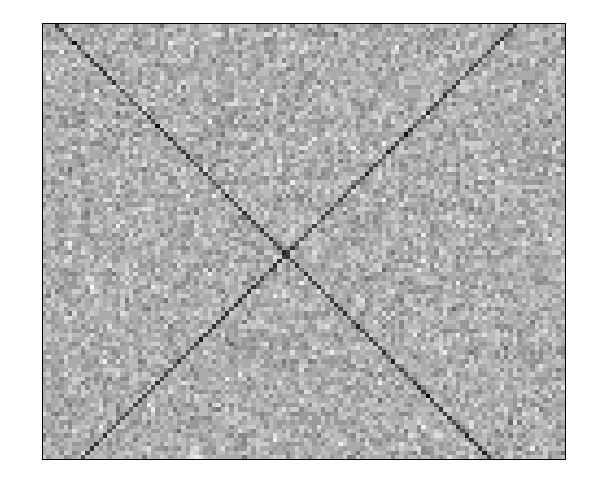
\includegraphics[width=\textwidth]{lines_noise}
        \caption{До алгоритма.}
        \label{fig:a_many_before}
    \end{subfigure}
        \quad
    \begin{subfigure}[b]{0.32\textwidth}
       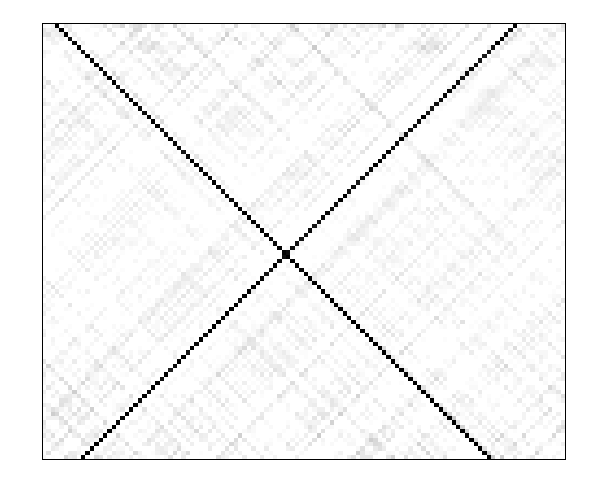
\includegraphics[width=\textwidth]{noauto_lines}
        \caption{После, без АИ.}
        \label{fig:a_many_after}
    \end{subfigure}
     \begin{subfigure}[b]{0.32\textwidth}
       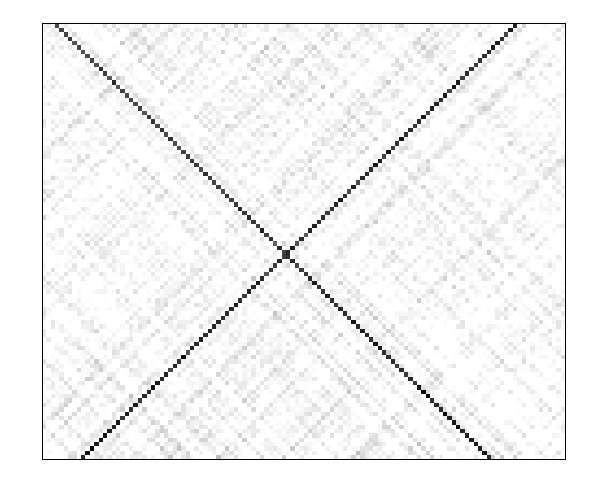
\includegraphics[width=\textwidth]{auto_lines}
        \caption{После, с АИ.}
        \label{fig:a_many_after2}
    \end{subfigure}
       \caption{Изображение с тремя линиями.}\label{fig:a_many}
\end{figure}

\chapter{Про реализацию методов автоматической идентификации}
Алгоритм \ref{alg:wcor} кластерного метода группировки и алгоритм \ref{alg:freq1d} метода низких частот для идентификации тренда для 1D-SSA  реализованы в R-пакетe \textsc{Rssa} \cite{Rssa, Golyandina.Korobeynikov2013}.

Алгоритм \ref{alg:1d_pgram} парного частотного метода, алгоритм \ref{alg:1dtau} метода по регулярности углов для идентификации колебательной составляющей для 1D-SSA был реализован самостоятельно, код реализации можно найти в ??.

Также в ?? реализованы все алгоритмы из главы \ref{sec:all_methods}.

%\conclusion
%Рассматривался вопрос обоснования автоматического метода идентификации э-м гармоник, предложенный в \cite{Zhornikova2016}.
%В работе получены следующие результаты.
%\begin{enumerate}
%\item Исследованы распределения значений $\tau_1(U_1, U_2)$ на примере э-м синуса и шума, приведены значения пересечений оценок плотностей этих распределений.
%\item Исследованы распределения значений $\tau_1(U_1, U_2)$ и $\tau_1(U_3, U_4)$ на примере зашумленного э-м синуса, приведены значения пересечений оценок плотностей этих распределений.
%\item Аналогично, как в пунктах 1 и 2 исследованы распределения для функционала $\tau_2$, только в этом случае использовалась чистая гармоника.
%\item Рассмотрен другой парный частотный метод автоматической идентификации, предложенный в \cite{Alexandrov2006} и \cite{Shmelov2011}. Метод реализован на языке R. Для меры этого метода проведены аналогичные исследования, как в пунктах 1 и 2, на тех же рядах. Проведено сравнение процента пересечения распределений мер, соответствующих сигналу и шуму, для парного частотного метода и метода, основанного на $\tau_1$. Последний алгоритм дал лучшие результаты.
%\item Проведено сравнение алгоритмов на модельных рядах для случая серии однотипных рядов.
%\end{enumerate}

\bibliographystyle{ugost2008}
\bibliography{biblio}

\appendix
\chapter{Сравнение методов автоматической идентификации колебательной компоненты для 1D-SSA}
\label{sec:compare}
В данном приложении, аналогично, как в разделе \ref{sec:tau_study} исследовали распределение меры $\tau$, исследуем распределение меры $\rho_{ij}$, заданной в \eqref{eq:rho_ij}, парного частотного метода из раздела \ref{sec:1d_pgram_method}. Также сравним парный частотный метод с методом по регулярности углов, основанного на использовании меры $\tau$, из главы \ref{sec:tau1}.
Моделирования проводились на тех же самых реализациях, что и для $\tau$.
%
%\section{Методы идентификации колебательной компоненты: периодограмный метод и метод, основанный на специальных функционалах}

\section{Исследование распределения меры для парного частотного метода}
\label{sec:per_study}

Будем использовать для моделирования те же ряды $\mathbb{S}$, $\mathbb{N}$ и $\mathbb{X}$ с элементами вида
\eqref{eq:series_S_N}, \eqref{eq:series_N_N}, \eqref{eq:series_X_N}, что и ранее в разделе \ref{sec:tau_study}.
$N = 99$, $L = 50$, моделировать будем $1000$ раз.

Исследуем распределение значений  меры $\rho_{1,2}$ для пары сингулярных векторов э-м гармоники $\mathbb{S}$ и для пары векторов шума $\mathbb{N}$, мера $\rho_{ij}$ определена в \eqref{eq:rho_ij}. Затем посмотрим на распределения  $\rho_{1,2}$ и  $\rho_{3,4}$ для ряда $\mathbb{X} = \mathbb{S} + \mathbb{N}$.

Рассматриваем $\alpha = 0.01$. Возьмем $\omega = 1/7$, т.е. $L\omega$ --- не целое.

Значения $\rho^{\mathbb{S}}_{1,2}$  для ряда $\mathbb{S}$ всегда будут одинаковыми и равными  $\rho^{\mathbb{S}}_{1,2} = 0.950$. Характеристики распределения $\rho^{\mathbb{N}}_{1,2}$ для ряда $\mathbb{N}$ для разных $\sigma$ представлены в таблице~\ref{tab:model_dist_pgram_sig2}.

\begin{table}[hhh!]
\caption{Распределение $\rho^{\mathbb{N}}_{1,2}$.}
\centering
\begin{tabular}{rrrrrrr}
  \hline
 & Min. & 1st Qu. & Median & Mean & 3rd Qu. & Max. \\
  \hline
$\sigma$=0.2 & 0.000 & 0.000 & 0.665 & 0.502 & 0.826 & 0.989 \\
  $\sigma$=0.4 & 0.000 & 0.000 & 0.685 & 0.525 & 0.840 & 0.986 \\
  $\sigma$=0.6 & 0.000 & 0.000 & 0.673 & 0.519 & 0.836 & 0.980 \\
  $\sigma$=0.8 & 0.000 & 0.000 & 0.682 & 0.524 & 0.833 & 0.985 \\
  $\sigma$=1 & 0.000 & 0.000 & 0.707 & 0.542 & 0.840 & 0.990 \\
   \hline
\end{tabular}
\label{tab:model_dist_pgram_sig2}
\end{table}

По таблице \ref{tab:model_dist_pgram_sig2} непонятно на сколько пересекаются распределения $\rho^{\mathbb{S}}_{1,2}$ и $\rho^{\mathbb{N}}_{1,2}$.
Аналогично как в разделе \ref{sec:tau_study} построим оценки плотностей распределений $\rho^{\mathbb{S}}_{1,2}$ и  $\rho^{\mathbb{N}}_{1,2}$ и посчитаем процент их пересечения.
Результаты представлены в таблице~\ref{tab:model_dist_pgram_overlap_222}. Распределения сильно пересекаются, на половину.

\begin{table}[hhh!]
\caption{Процент пересечения оценок плотностей для распределений $\rho^{\mathbb{S}}_{1,2}$ и $\rho^{\mathbb{N}}_{1,2}$.}
\centering
\begin{tabular}{rr}
  \hline
 & overlap\_$\rho$ \\
  \hline
$\sigma$ = 0.2 & 0.53 \\
  $\sigma$ = 0.4 & 0.55 \\
  $\sigma$ = 0.6 & 0.54 \\
  $\sigma$ = 0.8 & 0.55 \\
  $\sigma$ = 1 & 0.56 \\
   \hline
\end{tabular}
\label{tab:model_dist_pgram_overlap_222}
\end{table}

Посмотрим теперь на распределения  $\rho^{\mathbb{X}}_{1,2}$ и  $\rho^{\mathbb{X}}_{3,4}$ для ряда $\mathbb{X} = \mathbb{S} + \mathbb{N}$, представленные в таблицах ~\ref{tab:model_dist_pgram_sig_noise2} и \ref{tab:model_dist_pgram_sig_noise22}.

\begin{table}[hhh!]
\caption{Распределение $\rho^{\mathbb{X}}_{1,2}$.}
\centering
\begin{tabular}{rrrrrrr}
  \hline
 & Min. & 1st Qu. & Median & Mean & 3rd Qu. & Max. \\
  \hline
$\sigma$=0.2 & 0.927 & 0.945 & 0.949 & 0.949 & 0.953 & 0.967 \\
  $\sigma$=0.4 & 0.897 & 0.938 & 0.947 & 0.946 & 0.955 & 0.980 \\
  $\sigma$=0.6 & 0.868 & 0.932 & 0.946 & 0.944 & 0.957 & 0.988 \\
  $\sigma$=0.8 & 0.786 & 0.922 & 0.941 & 0.937 & 0.957 & 0.994 \\
  $\sigma$=1 & 0.000 & 0.904 & 0.932 & 0.923 & 0.952 & 0.997 \\
   \hline
\end{tabular}
\label{tab:model_dist_pgram_sig_noise2}
\end{table}

\begin{table}[hhh!]
\caption{Распределение $\rho^{\mathbb{X}}_{3,4}$.}
\centering
\begin{tabular}{rrrrrrr}
  \hline
 & Min. & 1st Qu. & Median & Mean & 3rd Qu. & Max. \\
  \hline
$\sigma$=0.2 & 0.000 & 0.000 & 0.670 & 0.508 & 0.838 & 0.982 \\
  $\sigma$=0.4 & 0.000 & 0.000 & 0.660 & 0.505 & 0.835 & 0.990 \\
  $\sigma$=0.6 & 0.000 & 0.000 & 0.655 & 0.507 & 0.835 & 0.990 \\
  $\sigma$=0.8 & 0.000 & 0.000 & 0.673 & 0.508 & 0.841 & 0.985 \\
  $\sigma$=1 & 0.000 & 0.000 & 0.650 & 0.492 & 0.829 & 0.977 \\
   \hline
\end{tabular}
\label{tab:model_dist_pgram_sig_noise22}
\end{table}

Построим оценки плотностей распределений $\rho^{\mathbb{X}}_{1,2}$  и  $\rho^{\mathbb{X}}_{3,4}$  и посчитаем процент их пересечения. Результаты представлены в таблице~\ref{tab:model_dist_pgram_overlap22}. При большом значении шума распределения пересекаются на 22 процента.
В таблице также приведены результаты для $\tau$ на тех же реализациях рядов.

\begin{table}[hhh!]
\caption{Процент пересечения оценок плотностей для распределений $\rho^{\mathbb{X}}_{1,2}$  и $\rho^{\mathbb{X}}_{3,4}$.}
\centering
\begin{tabular}{rrr}
  \hline
& overlap\_$\tau$& overlap\_$\rho$ \\
  \hline
$\sigma$ = 0.2 & 0.0004 & 0.037 \\
  $\sigma$ = 0.4 & 0.0013 & 0.082 \\
  $\sigma$ = 0.6 & 0.0035 & 0.123 \\
  $\sigma$ = 0.8 & 0.0182 & 0.171 \\
  $\sigma$ = 1 & 0.0716 & 0.220 \\
   \hline
\end{tabular}
\label{tab:model_dist_pgram_overlap22}
\end{table}
%
%\section{Таблицы пересечения оценок плотностей}
%
%
%%\subsection{$L\omega$ --- целое}
%
%Результаты для рядов $S_N$ и $R_N$ и мер от первых двух сингулярных векторов представлены в таблице \ref{tab:model_dist_all_Lomega_int}.
%
%\begin{table}[hhh!]
%\caption{Процент пересечения оценок плотностей распределений мер для рядов $S_N$ и $R_N$.}
%\centering
%\begin{tabular}{rrrrr}
%  \hline
% & $\tau$, $L\omega \in Z$ & pgram, $L\omega \in Z$  & $\tau$, $L\omega \not \in Z$  & pgram, $L\omega \not \in Z$  \\
%  \hline
%$\sigma$ = 0.2 & 0.00047 & 0.30 &  0.00144 & 0.53\\
%  $\sigma$ = 0.4 & 0.00046 & 0.30 & 0.00149 & 0.52\\
%  $\sigma$ = 0.6 & 0.00045 & 0.31 & 0.00152 & 0.53\\
%  $\sigma$ = 0.8 & 0.00051 & 0.31 &  0.00154 & 0.54 \\
%  $\sigma$ = 1 & 0.00050 & 0.32 & 0.00160 & 0.53 \\
%   \hline
%\end{tabular}
%\label{tab:model_dist_all_Lomega_int}
%\end{table}
%
%
%Результаты для ряда $X_N$ и мер от первых двух и следующих двух векторов представлены в таблице \ref{tab:model_dist_all_Lomega_int2}.
%
%\begin{table}[ht]
%\caption{Процент пересечения оценок плотностей распределений мер для ряда $X_N$.}
%\centering
%\begin{tabular}{rrrrr}
%  \hline
% & $\tau$, $L\omega \in Z$ & pgram, $L\omega \in Z$  & $\tau$, $L\omega \not \in Z$  & pgram, $L\omega \not \in Z$  \\
%  \hline
%$\sigma$ = 0.2 & 0.0003 & 0.007 &  0.0004 & 0.044 \\
%  $\sigma$ = 0.4 & 0.0011 & 0.021 & 0.0014 &  0.100\\
%  $\sigma$ = 0.6 & 0.0035 & 0.031 & 0.0036 & 0.141\\
%  $\sigma$ = 0.8 & 0.0184 & 0.068 & 0.0182 & 0.193\\
%  $\sigma$ = 1 & 0.0585 & 0.119 & 0.0683 & 0.244\\
%   \hline
%\end{tabular}
%\label{tab:model_dist_all_Lomega_int2}
%\end{table}
%
%Во всех случаях алгоритм с $\tau$ дает лучшие результаты.

\section{Сравнение парного частотного метода и метода по регулярности углов на модельных данных для случая серии однотипных рядов}
\label{sec:comp_tau1_pgram_many_same_series}
Как обычно, будем использовать для моделирования ряды $\mathbb{S}$, $\mathbb{N}$ и $\mathbb{X}$ с элементами вида
\eqref{eq:series_S_N}, \eqref{eq:series_N_N}, \eqref{eq:series_X_N}, что и ранее в разделе \ref{sec:tau_study}.
$N = 99$, $L = 50$, моделировать будем $1000$ раз.

Цель автоматической идентификации идентифицировать так же, как визуальная.
Поэтому сравним методы следующим способом.
Будем моделировать э-м гармонику $\mathbb{S}$ и шум $\mathbb{N}$ вида
c $\sigma = 0.2, 0.4, 0.6, 0.8, 1$, $\alpha = 0, 0.01$, $\omega = 1/7$ ($L\omega$ --- не целое).
%, $\varepsilon_k$ --- независимые случайные величины распределения $N(0,1)$. Берем $L = 24$. Взяли другие, чем ранее, значения $N$ и $L$ чтобы вычисления осуществлялись быстрее.
%Рассмотрим ряд $X_N = S_N + R_N$.
Для фиксированных значений параметров $\alpha$, $\omega$, $\sigma$ будем моделировать ряд $X_N = S_N + R_N$. Будем называться <<визуальной идентификации>> восстановление по первым двум компонентам.

Пусть $\mathbb{X}^{(1)}$ и $\mathbb{X}^{(2)}$ --- две реализации ряда $X_N$.
Пусть $\mathbb{S}^{(V,1)}$ и  $\mathbb{S}^{(V,2)}$ --- ряды, восстановленные по рядам $\mathbb{X}^{(1)}$ и $\mathbb{X}^{(2)}$ <<визуальной идентификацией>>.


Обозначаем значение порога для метода с $\tau$ через $t_0$, а для парного частотного метода через $\rho_0$. 
Пусть $\mathbb{S}^{(A,1,\varepsilon)}$ и  $\mathbb{S}^{(A,1, \rho_0)}$ --- ряды, восстановленные по ряду $X_N^{(1)}$  с помощью алгоритмов автоматической идентификации со значениями порогов $t_0$ и $\rho_0$ соответственно.
Также обозначим множество значений $T = \{0,0.01,0.02,\ldots, 0.99,1\}$, т.е. числа от $0$ до $1$ с шагом $0.01$.

Находим значения порогов $t_0^{opt}$ и $\rho_0^{opt}$, решая следующие задачи минимизации.

\begin{gather*}
t_0^{opt} = \argmin_{t_0 \in T}{\left(\frac{1}{N}\sum_{k=0}^{N-1}{\left(s_k^{(V,1)} - s_k^{(A,1,t_0)}\right)}^2\right)}, \\
\rho_0^{opt} = \argmin_{\rho_0 \in T}{\left(\frac{1}{N}\sum_{k=0}^{N-1}{\left(s_k^{(V,1)} - s_k^{(A,1,\rho_0)}\right)}    ^2\right)}.
\end{gather*}

Далее, пусть  $\mathbb{S}^{(A,2,\varepsilon^{opt})}$ и  $\mathbb{S}^{(A,2, \rho_0^{opt})}$ --- ряды, восстановленные по ряду $\mathbb{X}^{(2)}$  с помощью алгоритмов автоматической идентификации со значениями порогов $t_0^{opt}$ и $\rho_0^{opt}$ соответственно.

Посчитаем ошибки восстановления для этих рядов:
\begin{gather*}
E_{\tau} = \frac{1}{N}\sum_{k=0}^{N-1}{\left(s(k)^{(V,2)} - s(k)^{(A,2,t_0^{opt})}\right)^2}, \\
E_{\rho} = \frac{1}{N}\sum_{k=0}^{N-1}{\left(s(k)^{(V,2)} - s(k)^{(A,2,\rho_0^{opt})}\right)^2}.
\end{gather*}

Таким образом, мы посчитали оптимальное значение порога для одной реализации ряда $\mathbb{X}$ и с помощью этих оптимальных значений порогов восстановили ряды по второй реализации и посчитали ошибку восстановления для полученных рядов.

Повторим описанную процедуру $200$ раз и посчитаем среднее и медиану ошибок восстановления $E_{\tau}$ и $E_{\rho}$. Результаты для $\alpha = 0$, $\omega = 1/7$ представлены в таблице~\ref{tab:comp_tau1_pgram}. Результаты для $\alpha = 0.02$, $\omega = 1/7$ представлены в таблице~\ref{tab:comp_tau1_pgram2}.

\begin{table}[hhh!]
\centering
\caption{Сравнение алгоритмов при $\alpha = 0$, $\omega = 1/7$.}
\begin{tabular}{rrrrr}
  \hline
 & mean\_$\tau$ & mean\_$\rho$ & median\_$\tau$ & median\_$\rho$ \\
  \hline
  $\sigma$ = 0.2 & 0.0054 & 0.048 & 0 & 0.0000 \\
  $\sigma$ = 0.4 & 0.0237 & 0.063 & 0 & 0.0004 \\
  $\sigma$ = 0.6 & 0.0450 & 0.098 & 0 & 0.0369 \\
  $\sigma$ = 0.8 & 0.0804 & 0.163 & 0 & 0.0772 \\
  $\sigma$ = 1 & 0.0815 & 0.201 & 0 & 0.1207 \\
   \hline
\end{tabular}
\label{tab:comp_tau1_pgram}
\end{table}

\begin{table}[hhh!]
\centering
\caption{Сравнение алгоритмов при $\alpha = 0.02$, $\omega = 1/7$.}
\begin{tabular}{rrrrr}
  \hline
 & mean\_$\tau$ & mean\_$\rho$ & median\_$\tau$ & median\_$\rho$ \\
  \hline
$\sigma$ = 0.2 & 0.0011 & 0.045 & 0 & 0.0018 \\
  $\sigma$ = 0.4 & 0.0062 & 0.070 & 0 & 0.0061 \\
  $\sigma$ = 0.6 & 0.0041 & 0.096 & 0 & 0.0181 \\
  $\sigma$ = 0.8 & 0.0574 & 0.155 & 0 & 0.0389 \\
  $\sigma$ = 1 & 0.1802 & 0.279 & 0 & 0.1822 \\
   \hline
\end{tabular}
\label{tab:comp_tau1_pgram2}
\end{table}

%
%\chapter{Статья про анализ данных активности генов на английском языке} \label{sec:bio_article}
%\section{Introduction}
%The problem of measurement of between-nuclear variability is considered in many paper \cite{GeneExpression}.
%This variability consists of a pattern and noise. Two models of noise behaviour can be considered,
%the additive one, when the noise has constant variance, and the multiplicative model, when the standard deviation
%of noise is proportional to the pattern values.
%Detection, what model is valid, is very important for the noise analysis and for comparison of embryos, genes, ages...
%Therefore, an algorithm for discrimination of the models would be helpful.
%
%There are different kinds of data of gene expression activity.
%The original object is 3D. In \cite{Shlemov.etal2015.3D}, the extraction os a 3D patterns is performed
%by means of 3D singular spectrum analysis. One can seen that 3D analysis is very difficult; in particular,
%the choice of parameters, validation of the results and visualization need considerable efforts.
%In the same paper, an approach to detection of noise model is suggested.
%This approach is applicable to data of any dimension.
%
%More frequently, 2D data are considered, which are obtained by flattening embryos or by considering
%surface nuclei. The same approach with the use of 2D singular spectrum analysis to extraction of pattern
%is applied in \cite{Shlemov.etal2015.2D}.
%
%In this paper, we consider 2D data from \cite{GeneExpression} with gene expression activities
%for Kruppel and giant, Drosophila embryos of two ages, 4 and 8.
%Although 2D data are simpler than 3D for analysis, their accurate analysis
%is still complex. Moreover, the nuclei are non-equidistant and therefore
%the extraction procedure is complicated.
%
%One of standard ways to obtain 1D data from 2D data is to consider a thin stripe along
%the AP axis and then omit the DV coordinate. 1D data are more convenient, since it is
%much easy to depict, check the model validity, an so on.
%However, in the such approach, additional preprocessing errors arise.
%Since these errors are caused by errors in positions, they are connected
%with the derivative of the pattern: $u(x+\varepsilon)\approx u(x)+\varepsilon u'(x)$.
%If we are interested in the pattern, this effect is not important.
%However, if the level of expression noise is under interest (we will call it biological noise to differ from
%the processing noise), then the processing noise corrupts the noise level.
%
%The first problem, which is solved in the paper, is to construct the algorithm for estimation of the level of the
%biological noise in the presence of the processing noise.
%
%The other problem is how to measure the level of noise. If the biological noise
%is homogeneous and has the same level for all nuclei, then it can be measured as
%it standard deviation. This noise model is called additive: $g(x) = u(x) + \delta$.
%However, pictures of data show that probably it is not so.
%If the standard deviation of noise is proportional to the pattern values,
%then the corresponding noise model is called multiplicative: $g(x) = u(x)(1+\delta) = u(x) + u(x)\delta$.
%For multiplicative model, we should measure relative level of noise,
%that is, ratio of noise to pattern.
%
%Therefore, the second problem is to determine the noise model.
%
%Since the noise level can be estimated for 2D data (moreover, the noise
%model can be detected for 2D data), we compare the results for 1D and 2D processing.
%
%The paper is organized as follows.
%In Section 2, we consider models for 1D and 2D data.
%Section 2.1 is devoted to the model of 1D data, where the processing noise
%is added to additive or multiplicative models of the biological noise.
%The suggested algorithm is able to estimate standard deviations of
%both processing and biological noise.
%In Section 2.1.2, we introduce the algorithm for choosing between additive and
%multiplicative models.
%In Section 2.2 we briefly describe the model and the approach to 2D data.
%
%In Section 3, the constructed algorithms are tested by means of artificial 1D data,
%which are similar to real-life data for the Kruppel gene, and we apply the algorithms to 1D and 2D actual data, discuss and compare the results.
%
%Short discussion and conclusions are in Section 5.
%
%%
%%Consider 1D data, which are measured along a spatial axis X.
%%Suppose that the data has a pattern $u(x)$; there are errors
%%in $x$ and also the data consist of pattern and noise. The measurement noise (we will call it biological noise, since we will apply
%%the approach to the gene expression data) does not considered as an error and we are interested
%%is its model and variance.
%%
%%Thus, the observations have a form of a noisy pattern, where we are interested only in the part of the noise, which is caused by
%%some biological reasons.
%%The example of real-life data, which is considered in this paper, is the gene expression activity data taken from
%%\cite{GeneExpression}. Initially, these data are two-dimensional; however, a conventional approach is to
%%reduce them to 1D data to make their processing more easy.
%%
%%Note that the considered problem is not the standard regression problem with errors in arguments, when the estimation of
%%the pattern is under interest. In our case, the biological noise is of concern.
%
%\section{Methods}
%\label{sec:methods}
%\subsection{1D model estimation}
%\label{sec:methods_1D}
%\subsubsection{Estimation of $\sigma^2_x$ and $\sigma^2_y$}
%Let us formalize the problem. We consider two models (additive and multiplicative ones)
%with 1D pattern $u(x)$:
%\begin{eqnarray}
%\label{eq:add_approx}
%g_i = u(x_i) + \varepsilon_i w(x_i)  + \delta_i , \\ \label{eq:mult_approx}
%g_i = u(x_i) + \varepsilon_i(1+\delta_i)w(x_i) + \delta_i u(x_i),
%\end{eqnarray}
% where $i=0,\ldots, N-1$, $\varepsilon_i$ is a random variable with zero expectation and variance $\sigma^2_x$,
% $\delta_i$ is a random variable with zero expectation and variance $\sigma^2_y$;
% $\varepsilon_i$  and $\delta_i$ are independent.
%
%E.g., these models arise if there is an error in arguments, that is,
%if we measure $u$ in $x_i + \varepsilon_i$ instead of $x_i$. Then the approximation
%$u(x+\varepsilon_i) \approx u(x) + u'(x)\varepsilon_i$ yields \eqref{eq:add_approx} and \eqref{eq:mult_approx}
%with $w(x) = u'(x)$. Certainly, for this the approximation,
%the value $\sigma_x^2 |u''(x)| / 2$ should be small. Next we will consider $w(x) = u'(x)$.
%
%In both models, the data can be expressed as
%\begin{equation}
%\label{eq:common_model}
%g_i = u(x_i) + e_i
%\end{equation}
%and $\E g_i=u(x_i)$.
%Therefore, $(e_0, \ldots, e_{N-1})$ is the model noise of a complex form.
%Define $D(\sigma_x^2,\sigma_y^2) := \E e_i^2 = (\var(e_0),\ldots,\var(e_{N-1}))$.
%By analogy with time series, we call $(u_0,\ldots,u_{N-1})$, where $u_i = u(x_i)$, the signal.
%
%Our first task is is to construct algorithms for estimation of parameters $\sigma^2_x$ and $\sigma^2_y$ in both models. Then, we need to detect what model fits the data to choose the proper algorithm for parameter estimation.
%
%Note that the problem of noise variance estimation is considered in different papers, see e.g.  \cite{Brown2007} and references within.
%There are two approaches to variance estimation, through sequential differences \cite{Muller.Stadtmuller1987} and through local estimation of squared residuals averages \cite{Hall.Carroll1989}.
%We will construct our
%algorithms on the base of the second approach to take into consideration the specific of the models, where the noise modulation depends
%on the signal by a specific way.
% %However, we consider more complex model of noise; therefore, the methods like that from \cite{Brown2007} are not appropriate.
%
%
%\paragraph{Schemes of estimation of parameters $\sigma^2_x$ and $\sigma^2_y$}
%
%We first note that the noise from \eqref{eq:common_model} can be represented in the form
%\begin{equation} \label{eq:noise_regr}
%e_i^2 = \E e_i^2 + r_i = D(\sigma_x^2,\sigma_y^2) + r_i, \quad i=0,\ldots,N-1,
%\end{equation}
%where $\E r_i=0$, and $\var r_i$ depends on $\sigma^2_x$ and $\sigma^2_y$.
%
%$ D(\sigma_x^2,\sigma_y^2)$ from \eqref{eq:noise_regr} takes the form
%\begin{eqnarray*}
%D(\sigma_x^2,\sigma_y^2) = \sigma_x^2 w_i^2 + \sigma_y^2 \quad \textrm{for model \eqref{eq:add_approx}}, \\
%D(\sigma_x^2,\sigma_y^2) = \sigma_x^2 (1+\sigma_y^2) w_i^2 + \sigma_y^2 u_i^2  \quad \textrm{for  model \eqref{eq:mult_approx}},
%\end{eqnarray*}
%In vector form  \eqref{eq:noise_regr} can be written as
%\begin{eqnarray} \label{eq:regr_add}
%E^2= \sigma_x^2 D^2 + \sigma_y^2 + R \quad \textrm{for model \eqref{eq:add_approx}}, \\  \label{eq:regr_mult}
%E^2 = \sigma_x^2 (1+\sigma_y^2) D^2 + \sigma_y^2 T^2 + R^2 \quad \textrm{for  model \eqref{eq:mult_approx}}.
%\end{eqnarray}
%These formulas show that \eqref{eq:noise_regr} reduces to the problem of linear regression. If denoted $E = (e_0,\ldots,e_{N-1})$, $T = (u_0,\ldots,u_{N-1})$, $D = (w_0,\ldots,w_{N-1})$, then it will look like.
%
%\begin{equation} \label{eq:reg_common}
%Y = \mathbf{X}B + R,
%\end{equation}
%where
%\begin{itemize}
%\item $Y = (e^2_0,\ldots,e_{N-1}^2)^\mathrm{T}$;
%\item $\mathbf{X} = [X_1:X_2]$;
%% $X_1=D^2$, $X_2=~(1,\ldots,1)^\mathrm{T}$, $B=(\sigma_x^2,\sigma_y^2)^\mathrm{T}$ for model \eqref{eq:add_approx};\\
%%$X_1=D^2$, $X_2=T^2$,
%%$B~=~(\sigma_{x}^2(1+\sigma_y^2), \sigma_y^2)^\mathrm{T}$ for model \eqref{eq:mult_approx}.
%\item $R = (r_0,\ldots,r_{N-1})^\mathrm{T}$, $\covv{R} = \mathbf{W}$ depends on $B$;
%\end{itemize}
%and
%\begin{eqnarray}
%\label{eq:linreg_add}
%X_1=D^2, \,\,X_2=~(1,\ldots,1)^\mathrm{T}, \,\, B=(\sigma_x^2,\sigma_y^2)^\mathrm{T} \quad \textrm{for model \eqref{eq:add_approx}}; \\
%\label{eq:linreg_mult}
%X_1=D^2, \,\,X_2=~T^2, \,\, B=(\sigma_x^2,\sigma_y^2)^\mathrm{T} \quad \textrm{for model \eqref{eq:mult_approx}}.
%\end{eqnarray}
%
%Now let us present the algorithms of estimation of parameters $\sigma^2_x$ and $\sigma^2_y$ in both models.
%
%A scheme of estimation of parameters $\sigma^2_x$ and $\sigma^2_y$
% for the additive model is described in Algorithm \ref{alg1}, where \sigest{} denotes the signal estimation algorithm, \derivest{} denotes the derivation estimation algorithm and \linreg{} denotes the linear regression algorithm.
%
% \begin{algorithm}[!hhh]
%\caption{Estimation of variances in additive model in 1D case}
%\label{alg1}
%\begin{algorithmic}[1]
%\REQUIRE Values of  $g_i$, $x_i$, $i=0,\ldots,N-1$; algorithms: \sigest{}, \derivest{}, \linreg{}.
%\ENSURE The estimates of variances $\hat{\sigma}_x^2 $ and $\hat{\sigma}_y^2 $.
%\STATE Calling algorithms \sigest{} and \derivest{}. Their results are series  $\hat{T} = (\hat{u}_0,\ldots,\hat{u}_{N-1})$ and $\hat{D} = (\hat{w}_0,\ldots,\hat{w}_{N-1})$, respectively.
%\STATE Calculate the values $\hat{e}_i = g_i - \hat{u}(x_i)$. $\hat{E^2} = (\hat{e}^2_0,\ldots,\hat{e}^2_{N-1})$.
%\STATE Calling algorithm \linreg{} to solve the regression problem \eqref{eq:reg_common} with $\mathbf{X}$ from \eqref{eq:linreg_add}. Obtain the estimates $\hat{t}$ of intercept and the estimate $\hat{d}$ of the coefficient before $D^2$.
%\STATE Calculate the estimates of $\sigma_y^2$ and $\sigma_x^2$:
%$\hat{\sigma}_y^2 = \hat{t}$, $\hat{\sigma}_x^2 = \hat{d}$;
%\end{algorithmic}
%\end{algorithm}
%
%Using the estimates $\hat{\sigma}^2_x$ and $\hat{\sigma}^2_y$ obtained in the algorithm \ref{alg1}, we obtain the estimate of the model noise variance: $\hat{D}(\hat{\sigma}_x^2,\hat{\sigma}_y^2) = \hat\sigma^2_{y}  + \hat\sigma^2_{x} \,\hat{w}_i^2$.
%
%A scheme of estimation of  parameters $\sigma^2_x$ and $\sigma^2_y$
% for the multiplicative model is described in Algorithm \ref{alg2}, where \sigest{} is the signal estimation algorithm, \derivest{} is the derivation estimation algorithm and \linreg{} is the linear regression algorithm as for the additive model \eqref{eq:add_approx}.
%
%\begin{algorithm}[!hhh]
%\caption{Estimation of variances in multiplicative model in 1D case}
%\label{alg2}
%\begin{algorithmic}[1]
%\REQUIRE Values of  $g_i$, $x_i$, $i=0,\ldots,N-1$; algorithms: \sigest{}, \derivest{}, \linreg{}.
%\ENSURE The estimates of variances $\hat{\sigma}_x^2 $ and $\hat{\sigma}_y^2 $.
%\STATE Calling algorithms \sigest{} and \derivest{}. Their results are series  $\hat{T} = (\hat{u}_0,\ldots,\hat{u}_{N-1})$ and $\hat{D} = (\hat{w}_0,\ldots,\hat{w}_{N-1})$, respectively.
%\STATE Calculate the values $\hat{e}_i = g_i - \hat{u}(x_i)$. $\hat{E^2} = (\hat{e}^2_0,\ldots,\hat{e}^2_{N-1})$.
%\STATE Calling algorithm \linreg{} to solve the regression problem\eqref{eq:reg_common} with $\mathbf{X}$  from \eqref{eq:linreg_mult}. Obtain the estimates $\hat{t}$ of the coefficient before $T^2$
%and the estimate $\hat{d}$ of the coefficient before $D^2$.
%\STATE Calculate the estimates of $\sigma_y^2$ and $\sigma_x^2$:
%$\hat{\sigma}_y^2 = \hat{t}$,  $\hat{\sigma}_x^2 = \hat{d}/(1 + \hat{t})$;
%\end{algorithmic}
%\end{algorithm}
%
%Using the estimates $\hat{\sigma}^2_x$ and $\hat{\sigma}^2_y$ obtained in the algorithm \ref{alg2}, we obtain the estimate of the model noise variance: $\hat{D}(\hat{\sigma}_x^2,\hat{\sigma}_y^2) = \hat\sigma^2_{y}\, \hat{u}_i^2  + \hat\sigma^2_{x} (1+\hat{\sigma}_y^2) \,\hat{w}_i$.
%
%\paragraph{Solution of the regression problem}
%In the regression problems \eqref{eq:reg_common}, which are solved in items 3 of the Algorithms \ref{alg1} and \ref{alg2}, the model noise variance depends on the estimated parameters $\sigma_y^2$ and $\sigma_x^2$.
%Therefore, as \linreg algorithm we will use the iterative least-squares method (IRLS), see \cite{Daubechies2010}. The algorithm of IRLS has two parameters for
%the stopping rule: difference between two iterations $\tau$ and maximal number of iterations $M$, see Algorithm \ref{alg3}.
%
%\begin{algorithm}
%\caption{Iterative least-squares method for \eqref{eq:reg_common}}
%\label{alg3}
%\begin{algorithmic}[1]
%\REQUIRE matrix $\mathbf{X}$, vector $Y$; parameters: $\tau$, $M$.
%\ENSURE The vector of estimates $\widehat{B}$.
%\STATE Choice of the initial value $B_0$; $i \leftarrow 0$.
%\STATE Calculations of the weight matrix  $\mathbf{W}_{(i)}=\mathbf{W}(\widehat{B}_{(i)})$.
%  LS-estimation with the weight matrix $\mathbf{W}_{(i)}$:
%$\widehat{B}_{(i+1)}=(\mathbf{X}^\mathrm{T}\mathbf{W_{(i)}}^{-1}\mathbf{X})^{-1}\mathbf{X}^\mathrm{T}\mathbf{W}_{(i)}^{-1}Y$.
% \IF{$||\widehat{B}_{(i)}-\widehat{B}_{(i+1)}||<\tau$ or $i+1=M$} \STATE {STOP;} \STATE {$\widehat{B}=\widehat{B}_{(i+1)}$.} \ELSE \STATE{$i \leftarrow i+1$ and go to step 2.} \ENDIF
%\end{algorithmic}
%\end{algorithm}
%
%It is important to has linearly independent regressors to avoid degeneration of models.
%This means that in the additive model \eqref{eq:add_approx} the signal derivative should differ from a constant series;
%that is, for a linear signal, no estimates can be obtained. For the multiplicative model \eqref{eq:mult_approx},
% the signal derivative should not be a linear function of the signal;
% this means that
%for a exponential signal, no estimates can be obtained in the multiplicative model.
%
%
%\paragraph{Algorithms for estimation of the signal and its derivative}
%Next, we describe the algorithms for estimation of the signal and its derivative, which we will use as algorithms \sigest{} and \derivest{} in items 1 of the Algorithms \ref{alg1} and \ref{alg2}.
%
%For estimation of the signal $(u_0,\ldots,u_{N-1})$, we will consider the hybrid of Singular Spectrum Analysis (SSA \cite{Golyandina.etal2001})
%and local regression (LOESS \cite{Cleveland.etal1993}).
%
%The use of SSA for preprocessing is a conventional procedure, since SSA is nonparametric adaptive stable method, which does not need a-priori model of the signal and noise; see e.g.
%\cite{Golyandina.etal2001}.
%SSA has one main parameter $1<L<N$, which is called the window length. The method provides a decomposition of the initial object into
%a sum of elementary components. Then the estimate of the signal is equal to the sum of elementary components, which
%are identified as related to the signal.
%
%For automatic identification of elementary components, we will use the method described in \cite{Alexandrov2009} and Ref.~\cite[Section~2.4.5]{Golyandina.Zhigljavsky2012}. This method of identification has several parameters,
%the frequency  range $[\omega_1, \omega_2]$ and the threshold $t$.
%The method relates the component to the signal if its frequencies belong to $[\omega_1, \omega_2]$ and their  contribution is less than $t$. The value of the contribution can vary from $0$ to $1$.
%
% A drawback of SSA is that it ignores $x_i$ and processes the
%data as if they are equidistant, whereas $x_i$ may be non-equidistant.
%Therefore, an additional smoothing
%is necessary. Moreover, since derivatives $u'$ are estimated on the base on the estimated signal,
%the estimated signal should be smooth enough.
%
%Additional smoothing will be performed by the method LOESS($p$, $\beta$) with parameters $p$, which is the degree of the local polynomials,
% and $\beta$, which characterize the locality of smoothing. LOESS can deal with non-equidistant data.
%
% The described approach to signal estimation is presented in the Algorithm~\ref{alg4}.
%\begin{algorithm}
%\caption{Estimation of the signal in 1D case}
%\label{alg4}
%\begin{algorithmic}[1]
%\REQUIRE Values of  $g_i$, $x_i$, $i=0,\ldots,N-1$; parameters: $L$, $[\omega_1, \omega_2]$, $t$, $p$, $\beta$.
%\ENSURE Estimate of the signal $(\hat{u}_0, \ldots, \hat{u}_{N-1})$.
%\STATE Application of SSA to the series $(g_0, \ldots, g_{N-1})$ with the window length $L$ \\ and automatic grouping with the frequency  range $[\omega_1, \omega_2]$ and the threshold\\ $t$. The result is a series $( \tilde{g}_0, \ldots, \tilde{g}_{N-1})$.
%\STATE Application of LOESS($p$, $\beta$) to pairs of points $ \{x_0,\tilde{g}_0\}, \ldots, \{x_{N-1},\tilde{g}_{N-1}\}$.\\ The result is a estimate $(\hat{u}_0, \ldots, \hat{u}_{N-1})$.
%\end{algorithmic}
%\end{algorithm}
%
%For estimation of the derivative $w(x)=u'(x)$ at $x_i$ we will use the following formula of numerical differentiation
%(it is assumed that $x_i$ are ordered by increasing):
%\begin{equation*}\label{derivate}
%\tilde{w}(x_i) = \tilde{w}_i=\frac{\hat{u}_{i+1}-\hat{u}_{i-1}}{x_{i+1}-x_{i-1}}\ , \quad i=1,\ldots, N-2.
%\end{equation*}
%
%The result of the numerical differentiation we again smooth by means of LOESS($q$, $s$).
%
% The described approach to derivative estimation is presented in the Algorithm~\ref{alg5}.
%\begin{algorithm}
%\caption{Estimation of the derivative in 1D case}
%\label{alg5}
%\begin{algorithmic}[1]
%\REQUIRE Values of  $\hat{u}_i$, $x_i$, $i=0,\ldots,N-1$; parameters: $q$, $s$.
%\ENSURE Estimate of the derivative $(\hat{w}_0, \ldots, \hat{w}_{N-1})$.
%\STATE $\tilde{w}_i = (\hat{u}_{i+1}-\hat{u}_{i-1}) / (x_{i+1}-x_{i-1})$, $i=1,\ldots, N-2.$
%\STATE Application of LOESS($q$, $s$) to pairs of points $\{x_0,\tilde{w}_0\}, \ldots, \{x_{N-1},\tilde{w}_{N-1}\}$. The result is a estimate $(\hat{w}_0, \ldots, \hat{w}_{N-1})$.
%\end{algorithmic}
%\end{algorithm}
%
%\subsubsection{Model discrimination}
%Now let us consider the algorithm of discrimination between additive and multiplicative models. The additive noise corresponds to homoscedastic noise,
%while multiplicative noise corresponds to a special type of heteroscedastic noise with standard deviation, which is proportional to
%the signal values. To discriminate pure additive and multiplicative noises,
%the Park test \cite{Park1966} can be used.
%However, our models \eqref{eq:add_approx} and \eqref{eq:mult_approx} are neither pure additive nor pure multiplicative.
%
%%If a model does not contain errors in arguments, then there are different algorithms for model discrimination, which use the model noise $e_i$ from \eqref{eq:common_model}; see e.g. Park test \cite{Park1966}.
%%estimation of $\alpha$ in $g_i = u(x_i) + u^\alpha(x_i)\delta$. See e.g. \cite{Park1966}.
%%If $\alpha = 0$, then the model is additive; if $\alpha = 1$, then the model is multiplicative.
%%However, in the models \eqref{eq:add_approx} and \eqref{eq:mult_approx}, which are arised in the case
%%of e.g. error in arguments, these methods is not directly applied. For models \eqref{eq:add_approx}  and \eqref{eq:mult_approx}, the model noise \eqref{eq:common_model} has a complex shape.
%
%Thus, let us consider a heuristic algorithm. A straightforward approach is to compare mean systematic errors in the residuals of the regression from \eqref{eq:noise_regr} in both models.
%The main problems for measurement of systematic errors are that (1) the systematic error can have different signs for different $i$ and (2) the residuals in \eqref{eq:noise_regr} have different variances (noise is heteroscedastic). Therefore, we should estimate the bias locally and check its significance basing on the local estimates of the variance.
%%the residuals in \eqref{eq:noise_regr} are heteroscedastic and it is impossible to construct , and this does not allow us to distinguish the models using the residuals mean. Therefore, consider the bias as a function of $i$.
%%The main problem is that the models are hardly distinguished by the mean value of the
%%regression errors. Thereby, the suggested algorithm is based on the bias $r_i$ in the regression model \eqref{eq:noise_regr} at step 2 of the estimation algorithms.
%
%Thus, we consider the series $(\hat{r}_0, \ldots, \hat{r}_{N-1})$ of residuals obtained by means of  \eqref{eq:noise_regr}:
%$$
%\hat{r}_i = \hat{e}_i - \hat{D}(\sigma_x^2,\sigma_y^2),
%$$
%where $\hat{e}_i$ and $\hat{D}(\sigma_x^2,\sigma_y^2)$ were obtained in Algorithms \ref{alg1} and \ref{alg2}.
%If the model is not proper, then the residuals $r_i$ must have an bias.
%The idea is to measure this bias. The model with smaller bias is considered as proper model.
%
%The proposed algorithm consists of four steps.
%
%1. We apply to the series $(\hat{r}_0, \ldots, \hat{r}_{N-1})$ the moving median with window of length $3$, to remove possible outliers.
%Denote the resultant series  $(\bar{r}_0, \ldots, \bar{r}_{N-3})$.
%
%2.We choose $K$ and calculate the moving average and the moving standart deviation for the series $(\bar{r}_0, \ldots, \bar{r}_{N-3})$ with window of length $K$. We get the values $(\hat{m}_0,\ldots, \hat{m}_{N - K-2})$ and $(\hat{s}_0,\ldots, \hat{s}_{N - K-2})$, respectively.
%
%3. Based on the obtained values of $\hat{m}_i$ and $\hat{s}_i$, we construct confidence intervals for $\hat{m}_i$ with confidence level $\gamma$  for each $i = 0,\ldots, N-K-2$.
%Denote $c_i$ the bound of the intervals, which is closer to $0$, if the interval does not contain $0$, and $0$ otherwise.
%Thus, we obtain the series $(c_0,\ldots,c_{N-K-2})$ of length $N - K - 1$, which determines the bias.
%Formally,
%\begin{equation} \label{eq:c_i}
%c_i = \begin{cases}
%\min{\left(| \hat{m}_i \pm {z_{\gamma} \,\hat{s}_i/ \sqrt{K}} |\right)}, \,\,
%\mbox{if } 0 \not \in \left( \hat{m}_i \pm {z_{\gamma} \,\hat{s}_i/ \sqrt{K}}  \right);\\
%0, \,\, \mbox{otherwise},
%\end{cases}
%\end{equation}
% where $z_{\gamma}$ is $(1+\gamma)/2$-quantile of the standard normal distribution, $i = 0, \ldots, N - K - 2$.
%
%4. As a measure of agreement with the model, we consider the median of $(c_0,\ldots,c_{N - K - 2})$:
%\begin{equation} \label{eq:measure_mult_vs_add}
%c_\mathrm{med} = \med{(c_0,\ldots,c_{N -K - 2})}.
%\end{equation}
%
%A formal and brief description of this approach is given in Algorithm \ref{alg6}.
%\begin{algorithm}
%\caption{Model discrimination in 1D case}
%\label{alg6}
%\begin{algorithmic}[1]
%\REQUIRE Values of $\hat{r}_i$, $i=0,\ldots,N-1$; parameters $K$, $\gamma$.
%\ENSURE The value of the measure of agreement with the model $c_\mathrm{med}$.
%\STATE Application to the series $(\hat{r}_0, \ldots, \hat{r}_{N-1})$ of the moving median with window of length $3$. The resultant series  $(\bar{r}_0, \ldots, \bar{r}_{N-3})$.
%\STATE  Calculation the moving average and the variance for the series $(\bar{r}_0, \ldots, \bar{r}_{N-3})$ with window of length $K$. The resultant values $(\hat{m}_0,\ldots, \hat{m}_{N - K-2})$ and $(\hat{s}_0,\ldots, \hat{s}_{N - K-2})$, respectively.
%\STATE Obtaining confidence intervals for $\hat{m}_i$  with confidence level $\gamma$ for each $i = 0,\ldots, N-K-2$
%and the series $(c_0,\ldots,c_{N-K-2})$ of length $N - K - 1$, where $c_i$ from \eqref{eq:c_i}.
%\STATE The model with smaller $c_\mathrm{med}$ is a proper model.
%\end{algorithmic}
%\end{algorithm}
%
%\subsection{2D model estimation}
%Processing of 2D and 3D gene expression data is described in \cite{Shlemov.etal2015.2D} and \cite{Shlemov.etal2015.3D}.
%The algorithms are implemented in the R-package BioSSA \cite{BioSSA}.
%
%Since we assume that there are no errors in arguments for 2D data, then the models \eqref{eq:add_approx} and \eqref{eq:mult_approx}
%have a simplified form
%\begin{eqnarray}
%\label{eq:add_2D}
%g_i = u(\mathbf{x}_i) + \delta_i\\ \label{eq:mult_2D}
%g_i = u(\mathbf{x}_i)(1 + \delta_i),
%\end{eqnarray}
%where $\mathbf{x}_i \in \mathbb{R}^2$, $\delta_i$ is a random variable with zero expectation and variance  $\sigma_y^2$.
%
%\subsubsection{Estimation of $\sigma_y^2$}
%First, as in the 1D case, we estimate the parameter $\sigma_y^2$.
%The approach of estimation of variance $\sigma_y^2$ is described in Algorithm \ref{alg7}.
%
%\begin{algorithm}
%\caption{Estimation of $\sigma_y^2$ in 2D case}
%\label{alg7}
%\begin{algorithmic}[1]
%\REQUIRE Values of  $g_i$, $x_i$, $i=0,\ldots,N-1$, parameters: $L_1$, $L_2$,  $\Delta$.
%\ENSURE The estimate of variance $\hat{\sigma}_y^2 $.
%\STATE Interpolation of $\mathbf{x}_i$ to  regular rectangular grid with distance $\Delta$ between grid points.
%\STATE Application of 2D-SSA to the data on the regular grid with the parameter $L_1\times L_2$ (window size).
%\STATE Estimation of the signal on the base of the leading $r$ components of the decomposition
%produced by 2D-SSA.
%\STATE Back interpolation of the signal estimation to $\mathbf{x}_i$; residuals are calculated as
%$\hat{e}_i = g_i - \hat{u}(\mathbf{x}_i)$.
%\STATE $\hat\sigma_y^2 = \hat{e}_i^2$  for model \eqref{eq:add_2D}, $\hat\sigma_y^2 = \hat{e}_i^2/\hat{u}^2(\mathbf{x}_i)$  for model \eqref{eq:mult_2D}.
%\end{algorithmic}
%\end{algorithm}
%
%
%\subsubsection{Model discrimination}
%\label{sec:2D_disc}
%The models \eqref{eq:add_2D} and \eqref{eq:mult_2D} are particular cases of the model
%\begin{equation}
%\label{eq:2D_with_alpha}
%g_i = u(z_i) + u(z_i)^\alpha \delta_i.
%\end{equation}
%Values of $\alpha$, which are close to 1, means the the model is multiplicative, and values of $\alpha$, which are close to 0, means the the model is additive.
%In the 2D case, in contrast to the 1D case, the estimate $\sigma_y^2$  is not needed to discriminate models.
%We just need to estimate $\alpha$.
%
%We can
%estimate $\alpha$ in \eqref{eq:2D_with_alpha} by the Park method \cite{Park1966} as
%least-square estimator of $\alpha$ in the model
%$\log(|e_i|) = \alpha \log|\hat{u}(\mathbf{x}_i)| + r_i$.
%
%
%
% \section{Results. Application to gene expression activity}
% In this section, examples of application of the described methods to 2D data with gene expression activities for Drosophila embryos are given.
% The section \ref{sec:about_data} describes the structure of this data.
%
%In the section \ref{sec:app_model_data}, we test the approach and select parameters for Algorithms 1--7 by means of synthetical 1D and 2D data.
%%This data is needed in order to select parameters for Algorithms 1-7 from Section~\ref{sec:methods}.
% The pattern (signal) and noise level for these synthetical data are obtained from the gene expression data of several embryos.
%For algorithms 1--7 with parameters chosen with the help of artificial data are used in Sections \ref{sec:app_real_data_1D} and \ref{sec:app_real_data_2D} for processing of gene activity data.
%In the section \ref{sec:comp}, the results of processing 1D and 2D data are compared.
%
% \subsection{Data description}
% \label{sec:about_data}
%
%We take 2D data from \cite{GeneExpression} with gene expression activities
%for Kruppel and giant, Drosophila embryos of two ages, 4 and 8. Data was taken from the database FlyEx~\cite{FlyEx}.
%The number of embryos for different genes and ages is presented in Tabl.~\ref{tab:number_embryo}.
%
%\begin{table}[hhh!]
%\caption{The number of embryos for Kruppel and giant genes of two ages, 4 and 8.}
% \centering
% \begin{tabular}{rrrr}
%  \hline
%  &  Kruppel & giant \\
%  \hline
%  Age 4  & 36 & 18\\
%  Age 8  & 38 & 20\\
% \end{tabular}
% \label{tab:number_embryo}
% \end{table}
%
%The quantitative gene expression data was acquired from images of gene expression patterns obtained by confocal scanning microscopy of fixed embryos immunostained for segmentation proteins.
%Image segmentation recognizes nuclei from background. Each nucleus is characterized by the X and Y coordinates of its centroid, and the average fluorescence levels of three proteins scanned in the embryo.
%The data was transformed to the scale from 0 to 100\% by both dimensions, X and Y.
%For a more detailed description see \cite{FlyExArticle}.
%
%
% \subsection{Model discussion}
% \label{sec:about_model}
% We considered the 2D data as they are.
%1D data are obtained from 2D data by consideration of 10\% stripe along the X coordinate  with Y coordinate from 45\% to 55\%.
%Then the Y coordinate were omitted and the X coordinate was taken from 20\% to 80\%. An example of the data is depicted in Fig.~\ref{fig:real_data}. The figure shows the 1D data, as well as the estimated signal and noise.
%\begin{figure}[!hhh]
%	\begin{center}
%	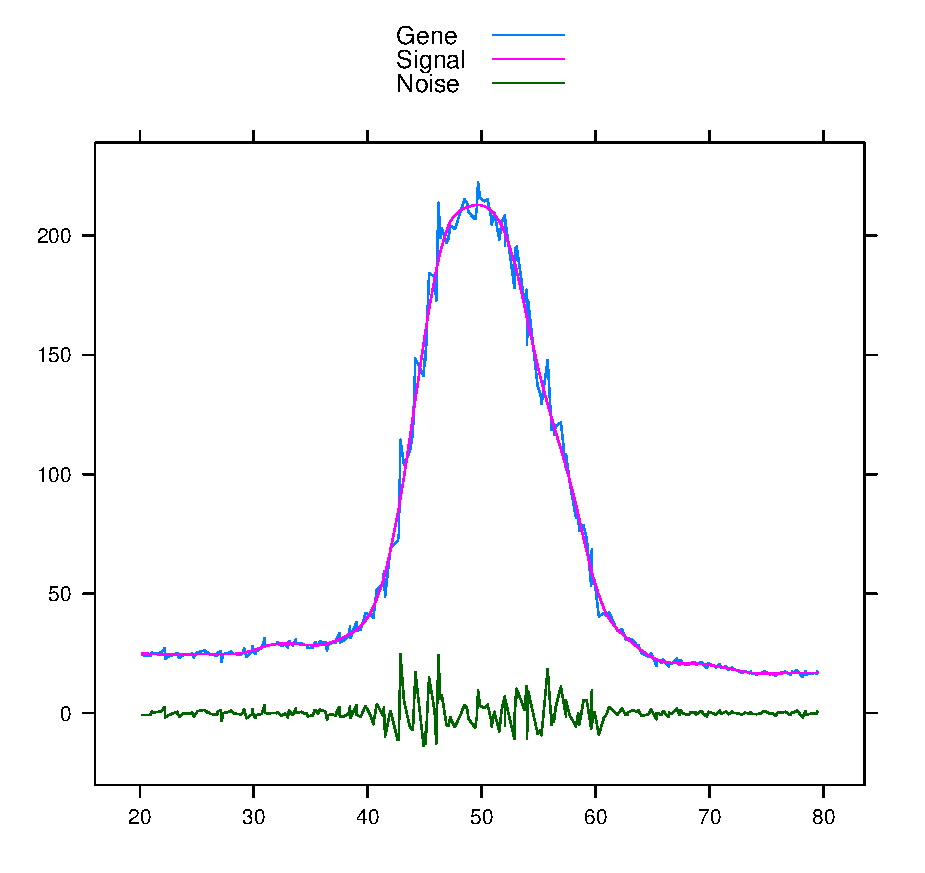
\includegraphics[width=2.5in]{real_data_trend_noise0}
%	\end{center}
%	\caption{An example of profile of the Kruppel gene, age 8, embryo bk1: gene activity data (blue), signal (pink), noise (green).}
%	\label{fig:real_data}
%\end{figure}
%
%An increase of the noise in the area of sharp changes of the pattern is clearly seen.
%We did not subtract the background, since it was already deleted in the database~\cite{FlyExArticle}.
%
%Let us note one important point in 1D case. When we omit the Y coordinate, we make a mistake along the Y-axis.
%We also make a mistake along the X-axis.
%But we will assume that we make a mistake only along the X-axis. Therefore, we need the values of the derivatives along X-axis and along Y-axis to be proportional, since $\varepsilon_i$ is present in the coefficient before the derivative in \eqref{eq:add_approx} and \eqref{eq:mult_approx}.
%Therefore, we considered the value of the cosine between the vectors composed of the derivatives along the X-axis and along the Y-axis. The average cosine value for all embryos is $0.85$.
%
%%On the one hand, 1D data have a simple form, and we will see later that our methods allow us to obtain good results for them. But 2D methods are simpler and allow more accurate results.
%
% \subsection{Application to artificial data}
% \label{sec:app_model_data}
%
% \paragraph{1D case}
%
%Let us investigate the suggested approach for artificial data, which repeat the behaviour of the gene expression activity.
%
%We use the pattern, which is extracted from a typical embryo bk1 (age 8), and the values of $x_i$ are taken from this data too. Then we simulate random noise fitted to either additive or multiplicative models as in \eqref{eq:add_approx} or \eqref{eq:mult_approx}, respectively.
%
%For the algorithms described in Section~\ref{sec:methods_1D} we take the following parameters.
%For IRLS (Algorithm \ref{alg3}), we take a small $\tau=10^{-8}$ and a large $M=200$. In practice IRLS converges much faster than for 200 iterations. For signal estimation (Algorithm \ref{alg4}), we take for SSA: small window size $L=30$ following the general recommendations in Ref.~\cite[Section~2.4.3]{Golyandina.Zhigljavsky2012}, frequency range $[\omega_1, \omega_2]=[0,0.04]$, threshold $t=0.4$. Frequency range $[0,0.04]$  means that we do not refer to the signal for oscillations with a period less than 25.
%For smoothing the signal by LOESS we set locality of smoothing $\beta=0.1$, degree of the local polynomials $p=2$ and the same values $s=0.1$, $q=2$ were taken for the additional smoothing of derivatives. This means that we approximate the data by quadratic polynomials and use 10\% of the data for each local polynomial.
%The quality of the selected parameters was checked visually in figures of the type shown in Fig.~\ref{fig:real_data}.
%
%For the creation of artificial data we take the following variance values.
%Take $\sigma_y^2=1$ for the additive model, $\sigma_y^2=0.0009$ for the multiplicative model and $\sigma_x^2 =0.1$ for both models. These parameters were selected on several embryos. These values are close to the average estimates of ${\sigma}_x^2$ and ${\sigma}_y^2$  for the actual data presented in sections \ref{sec:app_real_data_1D} for 1D case and \ref{sec:app_real_data_2D} for 2D case.
%
%Form of artificial data for both models is depicted in Fig.~\ref{fig:modeldata_f}.
%\begin{figure}
%	\centering
%    \begin{subfigure}[b]{0.45\textwidth}
%	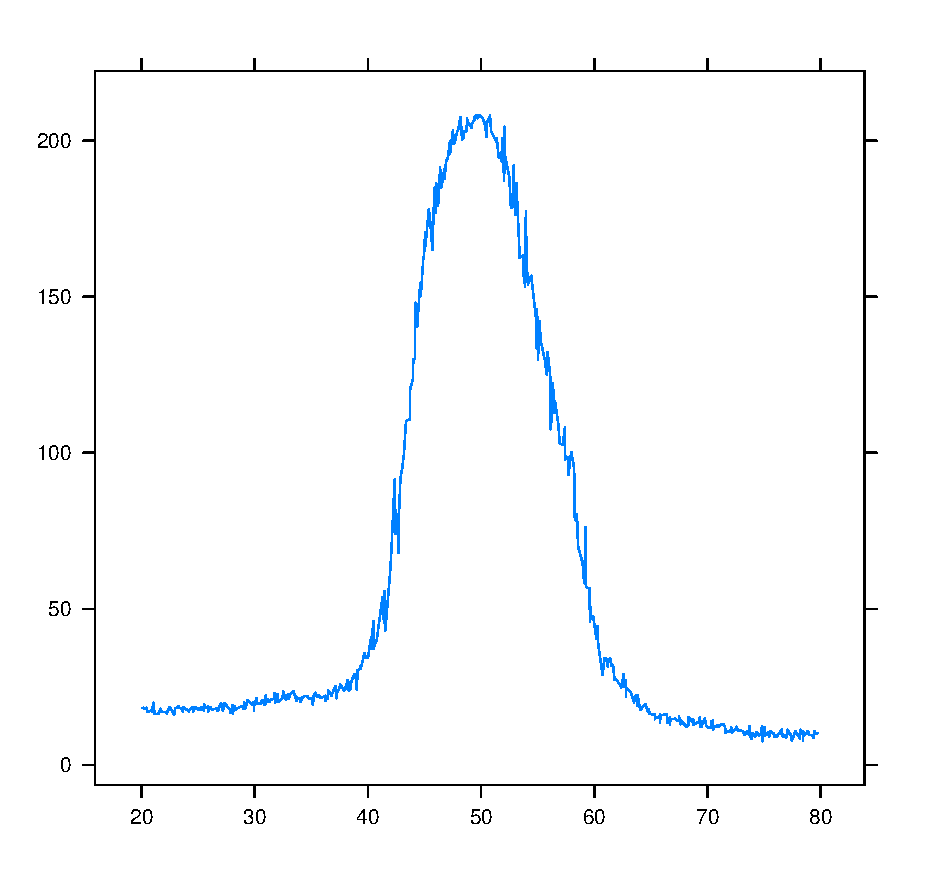
\includegraphics[scale=0.3]{add}
%	\caption{$f(x)$ in the additive case.}
%	\label{fig:modeldata_f_add}
%\end{subfigure}
%\quad
%    \begin{subfigure}[b]{0.45\textwidth}
%	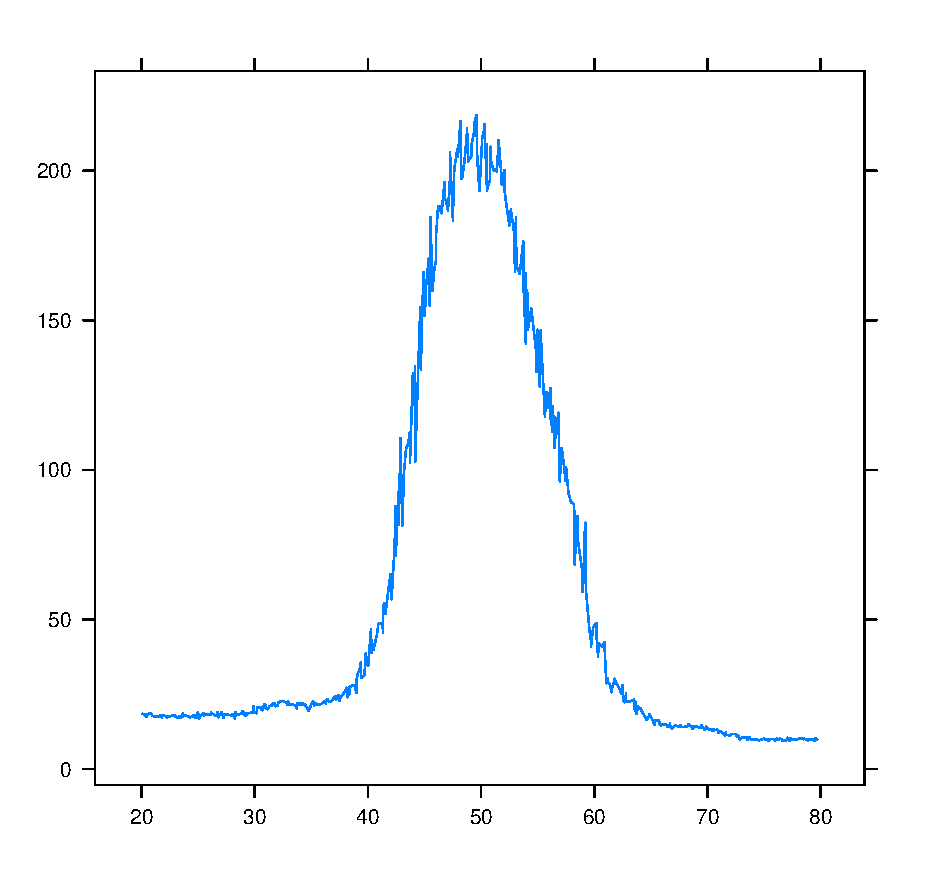
\includegraphics[scale=0.3]{mult}
%	\caption{$f(x)$ in the multiplicative case.}
%	\label{fig:modeldata_f_mult}
%\end{subfigure}
%\caption{An example of artificial data.}\label{fig:modeldata_f}
%\end{figure}
%
%We produced 200 simulations with (Gaussian) noise  with zero mean and variances $\sigma_x^2$ and $\sigma_y^2$ and obtained estimates $\hat{\sigma}_x^2$ and $\hat{\sigma}_y^2$.
%
%To show that it is important to consider the error along X-axis, we obtained yet another $\sigma_y^2$ estimate for conventional multiplicative model. We denote this estimate by  $\tilde{\sigma}_y^2$.
%
%  The results of estimation variances $\sigma_x^2$ and $\sigma_y$ for all cases are presented in the Tabl.~\ref{tab:mod_est_mult_mult_ssa_loess}.
% One can see that the estimates are bias. However, these biases are not large for $\hat{\sigma}_x^2$ and $\hat{\sigma}_y$.
%
%\begin{table}%[!hhh]
%\caption{Estimates of the variances $\sigma^2_{x}$ and $\sigma_{y}$ for the multiplicative model.}
% \centering
% \begin{tabular}{rrrrr}
%  \hline
%  & 1D $\sigma^2_{x}$ & 1D $\sigma_{y}$ & 1D $\tilde{\sigma}_{y}$  & 2D $\sigma_{y}$ \\
%  \hline
%  True values  & 0.100 & 0.03 & 0.03 & 0.03\\
%  Mean estimates  & 0.092 & 0.0285 & 0.0512 & 0.0311\\
%  Bias & 0.008 & 0.0015 & 0.0212 & 0.0011\\
%   sd & 0.0340 & 0.0036 & 0.0026 & 0.0006\\
% \end{tabular}
% \label{tab:mod_est_mult_mult_ssa_loess}
% \end{table}
%
%Now, using the obtained estimates $\hat{\sigma}_x^2$ and $\hat{\sigma}_y^2$, we apply the Algorithm \ref{alg6} for model discrimination. We take $K=51$ and $\gamma=0.05$.
%The discrimination of the models by the measure $c_\mathrm{med}$ defined in \eqref{eq:measure_mult_vs_add}
%(the data are referred to a model with the smallest measure) appears quite accurate.
%Right classification was performed in all cases for data generated by the multiplicative model and
%for 197 cases of 200 for data generated by the additive model.
%The bias of the estimates did not affect the quality of the classification.
%
%\paragraph{2D case}
%Similarly, as in the 1D case, we use the pattern, which is extracted from the embryo bk1 (age 8), and the values of $x_i$ are taken from this data too. Then we simulate random noise
%according to the multiplicative model
%\eqref{eq:mult_2D}.
%
%For this case, we use only Algorithm~\ref{alg7} from the section \ref{sec:methods}.
%Here we use 2D-SSA to the area $[20\%,80\%]\times [20\%,80\%]$ with the step for discretization $\Delta=0.5\%$.
%The choice of window sizes requires additional analysis, which we did.
%This preliminary analysis using the R-package BioSSA \cite{BioSSA} shows that the signal is described by the components 1--6.
%It is difficult to automatically identified the signal components, how it was done in the 1D case.
%Therefore, we choose typical values of the window size $10\times 10$.
%
%For the creation of artificial data we take $\sigma_y = 0.03$ (then $\sigma_y^2=0.0009$ as in 1D case).
%In accordance with the Section \ref{sec:2D_disc} in the 2D case, for discrimination of the model, it is not necessary to simulate both models, so here we do not simulate the additive model.
%
%We produced 200 simulations with (Gaussian) noise  with zero mean and variance $\sigma_y^2$.
%The mean values of estimates of $\sigma_y$ is equal to $0.031$.
%
%The mean values of estimates of $\alpha$ is equal to $0.98$, that is, the method is able to detect that the model is multiplicative.
%
%
%\paragraph{Comparison of results in 1D and 2D cases}
%Let us compare estimates in 1D and 2D cases.
%Mean estimates, standard deviation of estimates and bias in both cases are shown in Tabl.~\ref{tab:mod_est_mult_mult_ssa_loess}.
%
%We see that both estimates have a small bias, but the estimate for 2D has a smaller standard deviation.
%The main conclusion from the results is that if we are considering one-dimensional methods, then one should not forget about the error along the X-axis, otherwise the estimates of the variance $\sigma_y$ will be overestimated.
%
% \subsection{Application to 1D gene activity data}
% \label{sec:app_real_data_1D}
%
%Here we consider the set of embryos of two ages, 4 and 8, and the Kruppel and giant gene.
%
%The parameters of the Algorithms 1-6 from Section~\ref{sec:methods} are the same as were considered for the artificial data.
%
%Following to the approach, we estimate the estimates of the variances $\sigma^2_{x}$ and  $\sigma^2_{y}$ in both models
% and then refer the embryo to the model by comparison of the measure \eqref{eq:measure_mult_vs_add}.
%
%The estimates of $\sigma_{y}$ in the multiplicative model are presented in Tabl.~\ref{tab:real_est_compare_Kr} for Kruppel gene and Tabl.~\ref{tab:real_est_compare_gt} for giant gene.
% The average value of the estimate of  $\sigma^2_{x}$ for all embryos is $0.1$.
%
%For Kruppel gene, the model was classified as multiplicative for all embryos except one.
%For giant gene, the model was classified as multiplicative for all embryos.
% Thus we can conclude that the noise of gene expression is closer to multiplicative; that is, its level is proportional to the signal.
%
%
%\subsection{Application to 2D gene activity data}
%\label{sec:app_real_data_2D}
%Here we consider the set of embryos of two ages for 2D case.
%
%The parameters of the Algorithm 7 from Section~\ref{sec:methods} are the same as were considered for the artificial data.
%We apply 2D-SSA to the area $[20\%,80\%]\times [20\%,80\%]$ with the window $10\times 10$, the step for discretization $\Delta=0.5\%$ and 6 components for reconstruct.
%An example of the reconstruction and the residuals is depicted in Fig.~\ref{fig:ex_2d_rec} and Fig.~\ref{fig:ex_2d_res}.
%
%
%\begin{figure}
%	\centering
%    \begin{subfigure}[b]{0.45\textwidth}
%	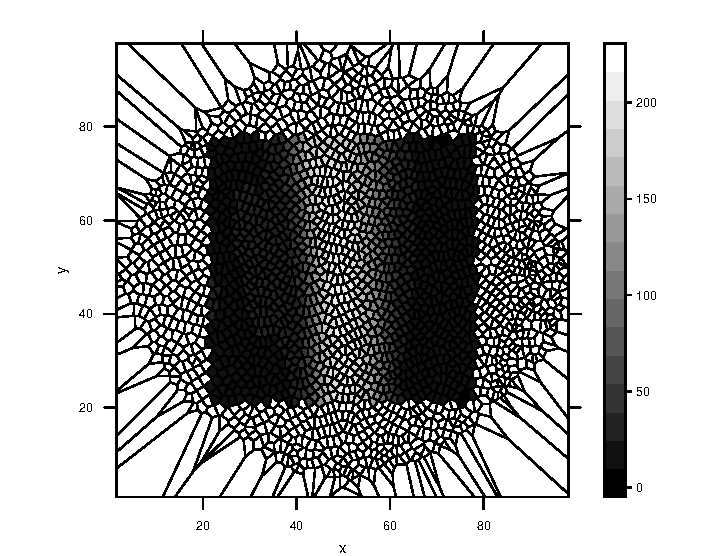
\includegraphics[scale=0.45]{bk1_rec.pdf}
%	\caption{Pattern of bk1}
%	\label{fig:ex_2d_rec}
%\end{subfigure}
%\quad
%    \begin{subfigure}[b]{0.45\textwidth}
%	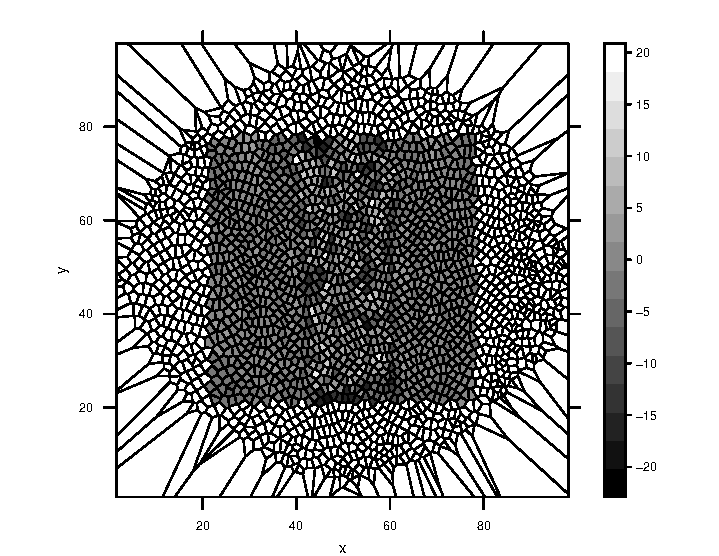
\includegraphics[scale=0.45]{bk1_res.pdf}
%	\caption{Residuals of bk1.}
%	\label{fig:ex_2d_res}
%\end{subfigure}
%\caption{An example of the reconstruction for bk1.}\label{fig:ex_2d}
%\end{figure}
%
%%\begin{figure}[!htb]
%%    \centering
%%    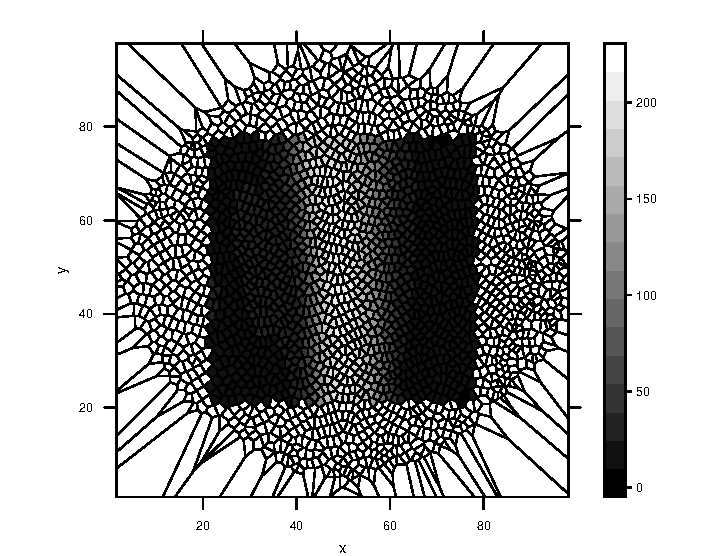
\includegraphics[width=3in]{bk1_rec.pdf} \\
%%    \caption{Pattern of bk1}
%%    \label{fig:ex_2d_rec}
%%\end{figure}
%%
%%\begin{figure}[!htb]
%%    \centering
%%    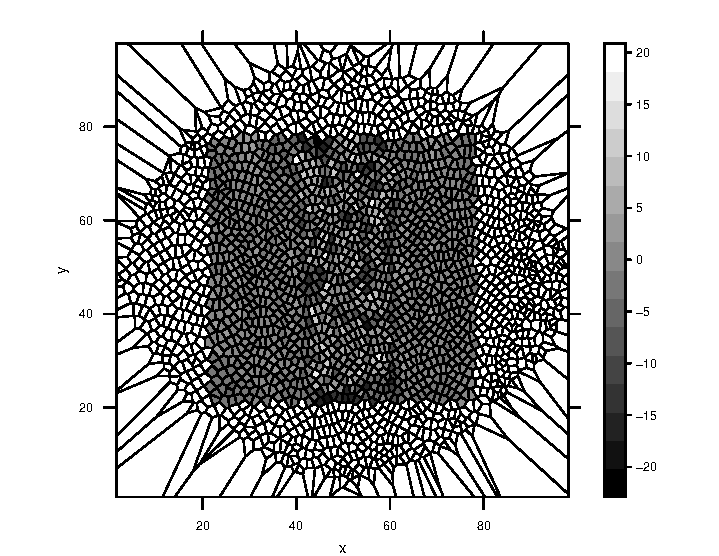
\includegraphics[width=3in]{bk1_res.pdf} \\
%%    \caption{Residuals of bk1}
%%    \label{fig:ex_2d_res}
%%\end{figure}
%
%For Kruppel gene, mean estimates of  $\sigma^2_{y}$ and $\alpha$ are: $0.027$ and $0.81$, for age 4.  For age 8, the corresponding values are $0.035$ and $1.01$. For giant gene, mean estimates of  $\sigma^2_{y}$ and $\alpha$ are: $0.028$ and $0.87$, for age 4.  For age 8, the corresponding values are $0.047$ and $1.11$.
%These results are also presented in Tabl.~\ref{tab:real_est_compare_Kr} and Tabl.~\ref{tab:real_est_compare_gt}.
%
%
%\subsection{Comparison}
%\label{sec:comp}
%
%Tables \ref{tab:real_est_compare_Kr} and \ref{tab:real_est_compare_gt} show the results of comparing the mean values of the estimates of $\sigma_y$ and their sd for the Kruppel and giant genes of two ages, 4 and 8, the number of which are presented in the Tabl.~\ref{tab:number_embryo}. From the results, one can see that for all genes and ages other than giant of age 8, estimates are of the same order, but in the 2D case the estimates have a smaller standart deviation.
%
%\begin{table}[hhh!]
%\caption{Comparison of estimates of the variance $\sigma_{y}$ for 1D and 2D data, Kruppel gene, ages 4 and 8.}
% \centering
% \begin{tabular}{rrrrr}
%  \hline
%  & 1D Kr 4 & 2D Kr 4  & 1D Kr 8 & 2D Kr 8\\
%  \hline
%  Mean estimates & 0.029 & 0.027 & 0.039 & 0.034 \\
%  sd & 0.010 & 0.007 & 0.012 & 0.006 \\
% \end{tabular}
% \label{tab:real_est_compare_Kr}
% \end{table}
%
% \begin{table}[hhh!]
%\caption{Comparison of estimates of the variance $\sigma_{y}$ for 1D and 2D data, giant gene, ages 4 and 8.}
% \centering
% \begin{tabular}{rrrrr}
%  \hline
%  & 1D gt 4 & 2D gt 4  & 1D gt 8 & 2D gt 8\\
%  \hline
%  Mean estimates & 0.031 & 0.028 & 0.063 & 0.047 \\
%  sd & 0.009 & 0.004 & 0.022 & 0.008 \\
% \end{tabular}
% \label{tab:real_est_compare_gt}
% \end{table}
%
%\section{Conclusion and discussion}
%We considered two approaches to noise estimation in 2D data, which are slowly varying along
%one of dimensions and therefore can be described by one-dimensional profiles.
%In the first approach, we consider a stripe in 2D data, which catches the pattern.
%In the second approach, we consider the 2D data as is.
%
%Our investigation shows that reasonable results can be obtained in both approaches.
%In the first 1D approach, it is much more easier to extract signals, estimate patterns
%and control the quality; on the other hand, the estimation is complicated, since
%we should take into consideration the processing errors and remove them.
%
%In the 2D approach, the accurate extraction of the pattern is difficult;
%on the other hand, the model is quite simple.
%
%We think that the further development of 2D and 3D methods is promising.
%However, the paper shows that if 1D data are analyzed, then it is very important
%to keep in mind the possible processing errors. These errors can be
%seen and oscillations whose level is proportional to the patter derivatives.
%
%The both approaches confirm that the considered data are closer to the multiplicative
%behaviour of the biological (gene expression) noise.
%
%%Я еще делала немного обратную ситуацию: моделировала $n$ раз ряд, и считала оптимальный порог для всех, выбирая тот порог, для которого ошибка с визуальной идентификацией была минимальна, потом все эти же ряды восстанавливала с помощью этого порога и оценивала ошибки первого, второго рода и пр. Надо ли это добавить? Итак уже много подтверждений, что наш метод лучше, на модельных данных.

\end{document}


